\documentclass[a4paper]{book}
\usepackage{makeidx}
\usepackage{natbib}
\usepackage{graphicx}
\usepackage{multicol}
\usepackage{float}
\usepackage{listings}
\usepackage{color}
\usepackage{ifthen}
\usepackage[table]{xcolor}
\usepackage{textcomp}
\usepackage{alltt}
\usepackage{ifpdf}
\ifpdf
\usepackage[pdftex,
            pagebackref=true,
            colorlinks=true,
            linkcolor=blue,
            unicode
           ]{hyperref}
\else
\usepackage[ps2pdf,
            pagebackref=true,
            colorlinks=true,
            linkcolor=blue,
            unicode
           ]{hyperref}
\usepackage{pspicture}
\fi
\usepackage[utf8]{inputenc}
\usepackage{mathptmx}
\usepackage[scaled=.90]{helvet}
\usepackage{courier}
\usepackage{sectsty}
\usepackage[titles]{tocloft}
\usepackage{doxygen}
\lstset{language=C++,inputencoding=utf8,basicstyle=\footnotesize,breaklines=true,breakatwhitespace=true,tabsize=8,numbers=left }
\makeindex
\setcounter{tocdepth}{3}
\renewcommand{\footrulewidth}{0.4pt}
\renewcommand{\familydefault}{\sfdefault}
\hfuzz=15pt
\setlength{\emergencystretch}{15pt}
\hbadness=750
\tolerance=750
\begin{document}
\hypersetup{pageanchor=false,citecolor=blue}
\begin{titlepage}
\vspace*{7cm}
\begin{center}
{\Large \-Interface }\\
\vspace*{1cm}
{\large \-Generated by Doxygen 1.7.6.1}\\
\vspace*{0.5cm}
{\small Wed Jul 1 2015 05:21:16}\\
\end{center}
\end{titlepage}
\clearemptydoublepage
\pagenumbering{roman}
\tableofcontents
\clearemptydoublepage
\pagenumbering{arabic}
\hypersetup{pageanchor=true,citecolor=blue}
\chapter{\-Namespace \-Index}
\section{\-Namespace \-List}
\-Here is a list of all documented namespaces with brief descriptions\-:\begin{DoxyCompactList}
\item\contentsline{section}{\hyperlink{namespaceutil}{util} \\*\-The namespace shared by all support classes that form lib\-Util }{\pageref{namespaceutil}}{}
\item\contentsline{section}{\hyperlink{namespaceutil_1_1common}{util\-::common} \\*\-The namespace shared by error classes in lib\-Util }{\pageref{namespaceutil_1_1common}}{}
\item\contentsline{section}{\hyperlink{namespaceutil_1_1math}{util\-::math} \\*\-The namespace containing all the math classes in lib\-Util }{\pageref{namespaceutil_1_1math}}{}
\end{DoxyCompactList}

\chapter{\-Class \-Index}
\section{\-Class \-Hierarchy}
\-This inheritance list is sorted roughly, but not completely, alphabetically\-:\begin{DoxyCompactList}
\item \contentsline{section}{\-Cell}{\pageref{classCell}}{}
\item \contentsline{section}{\-Correlation}{\pageref{classCorrelation}}{}
\item \contentsline{section}{\-Curve\-Points}{\pageref{classCurvePoints}}{}
\item \contentsline{section}{\-Descriptor}{\pageref{classDescriptor}}{}
\item \contentsline{section}{\-Drawn\-Skeleton}{\pageref{classDrawnSkeleton}}{}
\item \contentsline{section}{\-Entry}{\pageref{classEntry}}{}
\item \contentsline{section}{\-Equal\-Fn}{\pageref{classEqualFn}}{}
\item \contentsline{section}{util\-:\-:common\-:\-:error}{\pageref{classutil_1_1common_1_1error}}{}
\begin{DoxyCompactList}
\item \contentsline{section}{util\-:\-:common\-:\-:fatal\-\_\-error}{\pageref{classutil_1_1common_1_1fatal__error}}{}
\item \contentsline{section}{util\-:\-:common\-:\-:warning\-\_\-error}{\pageref{classutil_1_1common_1_1warning__error}}{}
\end{DoxyCompactList}
\item \contentsline{section}{\-Fail\-Safe}{\pageref{classFailSafe}}{}
\item \contentsline{section}{\-Frame\-Storage}{\pageref{classFrameStorage}}{}
\item \contentsline{section}{\-Grid}{\pageref{classGrid}}{}
\item \contentsline{section}{\-Hash}{\pageref{classHash}}{}
\item \contentsline{section}{\-Hasher}{\pageref{classHasher}}{}
\item \contentsline{section}{\-Histogram}{\pageref{classHistogram}}{}
\item \contentsline{section}{\-Image\-Votes}{\pageref{classImageVotes}}{}
\item \contentsline{section}{\-Index}{\pageref{classIndex}}{}
\item \contentsline{section}{\-Index\-Storage}{\pageref{classIndexStorage}}{}
\item \contentsline{section}{\-Main\-Window}{\pageref{classMainWindow}}{}
\item \contentsline{section}{util\-:\-:math\-:\-:mat33}{\pageref{classutil_1_1math_1_1mat33}}{}
\item \contentsline{section}{util\-:\-:math\-:\-:mat44}{\pageref{classutil_1_1math_1_1mat44}}{}
\item \contentsline{section}{\-Matching\-Image}{\pageref{classMatchingImage}}{}
\item \contentsline{section}{\-Oriented\-Image}{\pageref{classOrientedImage}}{}
\item \contentsline{section}{\-P\-O\-I\-N\-T}{\pageref{structPOINT}}{}
\item \contentsline{section}{\-Result\-Set}{\pageref{classResultSet}}{}
\item \contentsline{section}{\-Retrieved\-Skeleton}{\pageref{classRetrievedSkeleton}}{}
\item \contentsline{section}{\-Scribble\-Area}{\pageref{classScribbleArea}}{}
\item \contentsline{section}{\-Steerable}{\pageref{classSteerable}}{}
\item \contentsline{section}{\-Table}{\pageref{classTable}}{}
\item \contentsline{section}{\-Ui\-\_\-\-Dialog}{\pageref{classUi__Dialog}}{}
\begin{DoxyCompactList}
\item \contentsline{section}{\-Ui\-:\-:\-Dialog}{\pageref{classUi_1_1Dialog}}{}
\end{DoxyCompactList}
\item \contentsline{section}{\-Ui\-\_\-\-Main\-Window}{\pageref{classUi__MainWindow}}{}
\begin{DoxyCompactList}
\item \contentsline{section}{\-Ui\-:\-:\-Main\-Window}{\pageref{classUi_1_1MainWindow}}{}
\end{DoxyCompactList}
\item \contentsline{section}{util\-:\-:math\-:\-:vec2}{\pageref{classutil_1_1math_1_1vec2}}{}
\item \contentsline{section}{util\-:\-:math\-:\-:vec3}{\pageref{classutil_1_1math_1_1vec3}}{}
\item \contentsline{section}{util\-:\-:math\-:\-:vec4}{\pageref{classutil_1_1math_1_1vec4}}{}
\item \contentsline{section}{\-Weight\-Image}{\pageref{classWeightImage}}{}
\end{DoxyCompactList}

\chapter{\-Class \-Index}
\section{\-Class \-List}
\-Here are the classes, structs, unions and interfaces with brief descriptions\-:\begin{DoxyCompactList}
\item\contentsline{section}{\hyperlink{classDescriptor}{\-Descriptor} }{\pageref{classDescriptor}}{}
\item\contentsline{section}{\hyperlink{classEntry}{\-Entry} }{\pageref{classEntry}}{}
\item\contentsline{section}{\hyperlink{classEqualFn}{\-Equal\-Fn} }{\pageref{classEqualFn}}{}
\item\contentsline{section}{\hyperlink{classHash}{\-Hash} }{\pageref{classHash}}{}
\item\contentsline{section}{\hyperlink{classHasher}{\-Hasher} }{\pageref{classHasher}}{}
\item\contentsline{section}{\hyperlink{classHistogram}{\-Histogram} }{\pageref{classHistogram}}{}
\item\contentsline{section}{\hyperlink{classIndex}{\-Index} }{\pageref{classIndex}}{}
\item\contentsline{section}{\hyperlink{classIndexStorage}{\-Index\-Storage} }{\pageref{classIndexStorage}}{}
\item\contentsline{section}{\hyperlink{classResultSet}{\-Result\-Set} }{\pageref{classResultSet}}{}
\item\contentsline{section}{\hyperlink{classTable}{\-Table} }{\pageref{classTable}}{}
\end{DoxyCompactList}

\chapter{\-File \-Index}
\section{\-File \-List}
\-Here is a list of all documented files with brief descriptions\-:\begin{DoxyCompactList}
\item\contentsline{section}{/home/priyanka/\-Dataset25/src/db/\hyperlink{Descriptor_8h}{\-Descriptor.\-h} \\*\-This file contains values of descriptor and functions used to calculate and modify them }{\pageref{Descriptor_8h}}{}
\item\contentsline{section}{/home/priyanka/\-Dataset25/src/db/\hyperlink{Entry_8h}{\-Entry.\-h} \\*\-This file describe data structure for descriptor entries stored in database }{\pageref{Entry_8h}}{}
\item\contentsline{section}{/home/priyanka/\-Dataset25/src/db/\hyperlink{Hash_8h}{\-Hash.\-h} \\*\-This file describe data structure for hash function }{\pageref{Hash_8h}}{}
\item\contentsline{section}{/home/priyanka/\-Dataset25/src/db/\hyperlink{Histogram_8h}{\-Histogram.\-h} \\*\-This file store values of 3\-D histogram and functions to calculate and modify them }{\pageref{Histogram_8h}}{}
\item\contentsline{section}{/home/priyanka/\-Dataset25/src/db/\hyperlink{Index_8h}{\-Index.\-h} \\*\-This file describe data structure for descriptor entries stored in database }{\pageref{Index_8h}}{}
\item\contentsline{section}{/home/priyanka/\-Dataset25/src/db/{\bfseries \-Index\-Storage.\-h} }{\pageref{IndexStorage_8h}}{}
\item\contentsline{section}{/home/priyanka/\-Dataset25/src/db/\hyperlink{ResultSet_8h}{\-Result\-Set.\-h} \\*\-This file consist of matching result patches found for user drawn image }{\pageref{ResultSet_8h}}{}
\item\contentsline{section}{/home/priyanka/\-Dataset25/src/db/\hyperlink{Table_8h}{\-Table.\-h} \\*\-This file contain all the entries generated for different patches of all the images in database }{\pageref{Table_8h}}{}
\end{DoxyCompactList}

\chapter{\-Namespace \-Documentation}
\hypertarget{namespaceutil}{\section{util \-Namespace \-Reference}
\label{namespaceutil}\index{util@{util}}
}


\-The namespace shared by all support classes that form lib\-Util.  


\subsection*{\-Namespaces}
\begin{DoxyCompactItemize}
\item 
namespace \hyperlink{namespaceutil_1_1common}{common}
\begin{DoxyCompactList}\small\item\em \-The namespace shared by error classes in lib\-Util. \end{DoxyCompactList}\item 
namespace \hyperlink{namespaceutil_1_1math}{math}
\begin{DoxyCompactList}\small\item\em \-The namespace containing all the math classes in lib\-Util. \end{DoxyCompactList}\end{DoxyCompactItemize}


\subsection{\-Detailed \-Description}
\-The namespace shared by all support classes that form lib\-Util. \-Define \-P\-I if not present.

\-Define 2$\ast$\-P\-I if not present \-Min macro \-Max macro \-Degrees to radians conversion macro \-Radians to degrees macro \-Clamp a vlue between bounds macro 
\hypertarget{namespaceutil_1_1common}{\section{util\-:\-:common \-Namespace \-Reference}
\label{namespaceutil_1_1common}\index{util\-::common@{util\-::common}}
}


\-The namespace shared by error classes in lib\-Util.  


\subsection*{\-Classes}
\begin{DoxyCompactItemize}
\item 
class \hyperlink{classutil_1_1common_1_1error}{error}
\begin{DoxyCompactList}\small\item\em \-The general error class. \end{DoxyCompactList}\item 
class \hyperlink{classutil_1_1common_1_1fatal__error}{fatal\-\_\-error}
\begin{DoxyCompactList}\small\item\em \-The fatal error class. \end{DoxyCompactList}\item 
class \hyperlink{classutil_1_1common_1_1warning__error}{warning\-\_\-error}
\begin{DoxyCompactList}\small\item\em \-The warning error class. \end{DoxyCompactList}\end{DoxyCompactItemize}


\subsection{\-Detailed \-Description}
\-The namespace shared by error classes in lib\-Util. 
\hypertarget{namespaceutil_1_1math}{\section{util\-:\-:math \-Namespace \-Reference}
\label{namespaceutil_1_1math}\index{util\-::math@{util\-::math}}
}


\-The namespace containing all the math classes in lib\-Util.  


\subsection*{\-Classes}
\begin{DoxyCompactItemize}
\item 
class \hyperlink{classutil_1_1math_1_1vec2}{vec2}
\begin{DoxyCompactList}\small\item\em \-This is a general 2\-D vector class. \end{DoxyCompactList}\item 
class \hyperlink{classutil_1_1math_1_1vec3}{vec3}
\begin{DoxyCompactList}\small\item\em \-This is a general 3\-D vector class. \end{DoxyCompactList}\item 
class \hyperlink{classutil_1_1math_1_1vec4}{vec4}
\begin{DoxyCompactList}\small\item\em \-This is a general 4\-D vector class. \end{DoxyCompactList}\item 
class \hyperlink{classutil_1_1math_1_1mat33}{mat33}
\begin{DoxyCompactList}\small\item\em \-This is a general 3x3 matrix class. \end{DoxyCompactList}\item 
class \hyperlink{classutil_1_1math_1_1mat44}{mat44}
\begin{DoxyCompactList}\small\item\em \-This is a general 4x4 matrix class. \end{DoxyCompactList}\end{DoxyCompactItemize}
\subsection*{\-Enumerations}
\begin{DoxyCompactItemize}
\item 
enum \{ {\bfseries \-X}, 
{\bfseries \-Y}, 
{\bfseries \-Z}, 
{\bfseries \-W}
 \}
\begin{DoxyCompactList}\small\item\em \-The \-X,\-Y,\-Z,\-W coordinates. \end{DoxyCompactList}\end{DoxyCompactItemize}
\subsection*{\-Functions}
\begin{DoxyCompactItemize}
\item 
\hypertarget{namespaceutil_1_1math_af8c34d2c58bade9c6ff7f177252b9461}{\hyperlink{classutil_1_1math_1_1vec2}{vec2} {\bfseries operator-\/} (const \hyperlink{classutil_1_1math_1_1vec2}{vec2} \&v)}\label{namespaceutil_1_1math_af8c34d2c58bade9c6ff7f177252b9461}

\item 
\hypertarget{namespaceutil_1_1math_a62f2dd7ec9c7cb54e47cad2e1773d8ad}{\hyperlink{classutil_1_1math_1_1vec2}{vec2} {\bfseries operator+} (const \hyperlink{classutil_1_1math_1_1vec2}{vec2} \&v1, const \hyperlink{classutil_1_1math_1_1vec2}{vec2} \&v2)}\label{namespaceutil_1_1math_a62f2dd7ec9c7cb54e47cad2e1773d8ad}

\item 
\hypertarget{namespaceutil_1_1math_a1443696768a3f5191c706011f0933fd2}{\hyperlink{classutil_1_1math_1_1vec2}{vec2} {\bfseries operator-\/} (const \hyperlink{classutil_1_1math_1_1vec2}{vec2} \&v1, const \hyperlink{classutil_1_1math_1_1vec2}{vec2} \&v2)}\label{namespaceutil_1_1math_a1443696768a3f5191c706011f0933fd2}

\item 
\hypertarget{namespaceutil_1_1math_a082d1ad4a6150b421716c9235f06fb12}{\hyperlink{classutil_1_1math_1_1vec2}{vec2} {\bfseries operator$\ast$} (const \hyperlink{classutil_1_1math_1_1vec2}{vec2} \&v, const double d)}\label{namespaceutil_1_1math_a082d1ad4a6150b421716c9235f06fb12}

\item 
\hypertarget{namespaceutil_1_1math_ae6064900863ad9860577841b2045b84c}{\hyperlink{classutil_1_1math_1_1vec2}{vec2} {\bfseries operator$\ast$} (const double d, const \hyperlink{classutil_1_1math_1_1vec2}{vec2} \&v)}\label{namespaceutil_1_1math_ae6064900863ad9860577841b2045b84c}

\item 
\hypertarget{namespaceutil_1_1math_af69bff2e1e0f481e05c63d43f97a7bdf}{double {\bfseries operator$\ast$} (const \hyperlink{classutil_1_1math_1_1vec2}{vec2} \&v1, const \hyperlink{classutil_1_1math_1_1vec2}{vec2} \&v2)}\label{namespaceutil_1_1math_af69bff2e1e0f481e05c63d43f97a7bdf}

\item 
\hypertarget{namespaceutil_1_1math_aa4d9e8507ce0bb4411034df2ba1afa71}{\hyperlink{classutil_1_1math_1_1vec2}{vec2} {\bfseries operator/} (const \hyperlink{classutil_1_1math_1_1vec2}{vec2} \&v, const double d)}\label{namespaceutil_1_1math_aa4d9e8507ce0bb4411034df2ba1afa71}

\item 
\hypertarget{namespaceutil_1_1math_a52edab5fab276b3bd8a07d3b71df618e}{\hyperlink{classutil_1_1math_1_1vec3}{vec3} {\bfseries operator$^\wedge$} (const \hyperlink{classutil_1_1math_1_1vec2}{vec2} \&v1, const \hyperlink{classutil_1_1math_1_1vec2}{vec2} \&v2)}\label{namespaceutil_1_1math_a52edab5fab276b3bd8a07d3b71df618e}

\item 
\hypertarget{namespaceutil_1_1math_aa7db415cf980effc574394e4b8bdcf78}{bool {\bfseries operator==} (const \hyperlink{classutil_1_1math_1_1vec2}{vec2} \&v1, const \hyperlink{classutil_1_1math_1_1vec2}{vec2} \&v2)}\label{namespaceutil_1_1math_aa7db415cf980effc574394e4b8bdcf78}

\item 
\hypertarget{namespaceutil_1_1math_a4da0807ac8b804c97da35d37dd0537e5}{bool {\bfseries operator!=} (const \hyperlink{classutil_1_1math_1_1vec2}{vec2} \&v1, const \hyperlink{classutil_1_1math_1_1vec2}{vec2} \&v2)}\label{namespaceutil_1_1math_a4da0807ac8b804c97da35d37dd0537e5}

\item 
\hypertarget{namespaceutil_1_1math_adffadfb69d346d74c03ee8d6699cca4e}{void {\bfseries swap} (\hyperlink{classutil_1_1math_1_1vec2}{vec2} \&v1, \hyperlink{classutil_1_1math_1_1vec2}{vec2} \&v2)}\label{namespaceutil_1_1math_adffadfb69d346d74c03ee8d6699cca4e}

\item 
\hypertarget{namespaceutil_1_1math_ad6232f566ca99d968c0bb9a321d354df}{\hyperlink{classutil_1_1math_1_1vec2}{vec2} {\bfseries min} (const \hyperlink{classutil_1_1math_1_1vec2}{vec2} \&v1, const \hyperlink{classutil_1_1math_1_1vec2}{vec2} \&v2)}\label{namespaceutil_1_1math_ad6232f566ca99d968c0bb9a321d354df}

\item 
\hypertarget{namespaceutil_1_1math_a1a3845e6dd91197df2f28cc0325e1e3f}{\hyperlink{classutil_1_1math_1_1vec2}{vec2} {\bfseries max} (const \hyperlink{classutil_1_1math_1_1vec2}{vec2} \&v1, const \hyperlink{classutil_1_1math_1_1vec2}{vec2} \&v2)}\label{namespaceutil_1_1math_a1a3845e6dd91197df2f28cc0325e1e3f}

\item 
\hypertarget{namespaceutil_1_1math_a784fe3f27add234581b633c79482daf3}{\hyperlink{classutil_1_1math_1_1vec2}{vec2} {\bfseries prod} (const \hyperlink{classutil_1_1math_1_1vec2}{vec2} \&v1, const \hyperlink{classutil_1_1math_1_1vec2}{vec2} \&v2)}\label{namespaceutil_1_1math_a784fe3f27add234581b633c79482daf3}

\item 
\hypertarget{namespaceutil_1_1math_ae7da481caabecd445e92b3d229f5cf1a}{\hyperlink{classutil_1_1math_1_1vec3}{vec3} {\bfseries operator-\/} (const \hyperlink{classutil_1_1math_1_1vec3}{vec3} \&v)}\label{namespaceutil_1_1math_ae7da481caabecd445e92b3d229f5cf1a}

\item 
\hypertarget{namespaceutil_1_1math_a6ac2ed233b260a802034c0c3b00e5f49}{\hyperlink{classutil_1_1math_1_1vec3}{vec3} {\bfseries operator+} (const \hyperlink{classutil_1_1math_1_1vec3}{vec3} \&v1, const \hyperlink{classutil_1_1math_1_1vec3}{vec3} \&v2)}\label{namespaceutil_1_1math_a6ac2ed233b260a802034c0c3b00e5f49}

\item 
\hypertarget{namespaceutil_1_1math_a67d88d79f5d05c9e144a63392fccd4e5}{\hyperlink{classutil_1_1math_1_1vec3}{vec3} {\bfseries operator-\/} (const \hyperlink{classutil_1_1math_1_1vec3}{vec3} \&v1, const \hyperlink{classutil_1_1math_1_1vec3}{vec3} \&v2)}\label{namespaceutil_1_1math_a67d88d79f5d05c9e144a63392fccd4e5}

\item 
\hypertarget{namespaceutil_1_1math_aa7be0353b6e530e374face2cc4350408}{\hyperlink{classutil_1_1math_1_1vec3}{vec3} {\bfseries operator$\ast$} (const \hyperlink{classutil_1_1math_1_1vec3}{vec3} \&v, const double d)}\label{namespaceutil_1_1math_aa7be0353b6e530e374face2cc4350408}

\item 
\hypertarget{namespaceutil_1_1math_a51e44a08bd87589ec6a90bd866519af1}{\hyperlink{classutil_1_1math_1_1vec3}{vec3} {\bfseries operator$\ast$} (const double d, const \hyperlink{classutil_1_1math_1_1vec3}{vec3} \&v)}\label{namespaceutil_1_1math_a51e44a08bd87589ec6a90bd866519af1}

\item 
\hypertarget{namespaceutil_1_1math_a5066c6f085c5c32c7b784849e6fa2b0e}{\hyperlink{classutil_1_1math_1_1vec3}{vec3} {\bfseries operator$\ast$} (const \hyperlink{classutil_1_1math_1_1vec3}{vec3} \&v, \hyperlink{classutil_1_1math_1_1mat33}{mat33} \&\-M)}\label{namespaceutil_1_1math_a5066c6f085c5c32c7b784849e6fa2b0e}

\item 
\hypertarget{namespaceutil_1_1math_aafbed4062b22e4ddd321473f9645d406}{\hyperlink{classutil_1_1math_1_1vec3}{vec3} {\bfseries operator$\ast$} (\hyperlink{classutil_1_1math_1_1mat33}{mat33} \&\-M, const \hyperlink{classutil_1_1math_1_1vec3}{vec3} \&v)}\label{namespaceutil_1_1math_aafbed4062b22e4ddd321473f9645d406}

\item 
\hypertarget{namespaceutil_1_1math_a6e2063b3b086eca56dec26a4b1a389b5}{double {\bfseries operator$\ast$} (const \hyperlink{classutil_1_1math_1_1vec3}{vec3} \&v1, const \hyperlink{classutil_1_1math_1_1vec3}{vec3} \&v2)}\label{namespaceutil_1_1math_a6e2063b3b086eca56dec26a4b1a389b5}

\item 
\hypertarget{namespaceutil_1_1math_aa631e9bcbe2dc8e658ccf2c923963fde}{\hyperlink{classutil_1_1math_1_1vec3}{vec3} {\bfseries operator/} (const \hyperlink{classutil_1_1math_1_1vec3}{vec3} \&v, const double d)}\label{namespaceutil_1_1math_aa631e9bcbe2dc8e658ccf2c923963fde}

\item 
\hypertarget{namespaceutil_1_1math_a246900c73a1a0fc0d968e6be056f9320}{\hyperlink{classutil_1_1math_1_1vec3}{vec3} {\bfseries operator$^\wedge$} (const \hyperlink{classutil_1_1math_1_1vec3}{vec3} \&v1, const \hyperlink{classutil_1_1math_1_1vec3}{vec3} \&v2)}\label{namespaceutil_1_1math_a246900c73a1a0fc0d968e6be056f9320}

\item 
\hypertarget{namespaceutil_1_1math_aa7104771161ee13e849648ad7a46a8a5}{bool {\bfseries operator==} (const \hyperlink{classutil_1_1math_1_1vec3}{vec3} \&v1, const \hyperlink{classutil_1_1math_1_1vec3}{vec3} \&v2)}\label{namespaceutil_1_1math_aa7104771161ee13e849648ad7a46a8a5}

\item 
\hypertarget{namespaceutil_1_1math_a4c54929a74e44b52c59c1c7991367277}{bool {\bfseries operator!=} (const \hyperlink{classutil_1_1math_1_1vec3}{vec3} \&v1, const \hyperlink{classutil_1_1math_1_1vec3}{vec3} \&v2)}\label{namespaceutil_1_1math_a4c54929a74e44b52c59c1c7991367277}

\item 
\hypertarget{namespaceutil_1_1math_a131976d3a01db92180317ab8f379e65c}{void {\bfseries swap} (\hyperlink{classutil_1_1math_1_1vec3}{vec3} \&v1, \hyperlink{classutil_1_1math_1_1vec3}{vec3} \&v2)}\label{namespaceutil_1_1math_a131976d3a01db92180317ab8f379e65c}

\item 
\hypertarget{namespaceutil_1_1math_ad58c3a2902ce57818ab50ecbfc03a131}{\hyperlink{classutil_1_1math_1_1vec3}{vec3} {\bfseries min} (const \hyperlink{classutil_1_1math_1_1vec3}{vec3} \&v1, const \hyperlink{classutil_1_1math_1_1vec3}{vec3} \&v2)}\label{namespaceutil_1_1math_ad58c3a2902ce57818ab50ecbfc03a131}

\item 
\hypertarget{namespaceutil_1_1math_aa076e1c0d7a095302dc433faf9c46d56}{\hyperlink{classutil_1_1math_1_1vec3}{vec3} {\bfseries max} (const \hyperlink{classutil_1_1math_1_1vec3}{vec3} \&v1, const \hyperlink{classutil_1_1math_1_1vec3}{vec3} \&v2)}\label{namespaceutil_1_1math_aa076e1c0d7a095302dc433faf9c46d56}

\item 
\hypertarget{namespaceutil_1_1math_ae68cd56178c408e585e473afc430858f}{\hyperlink{classutil_1_1math_1_1vec3}{vec3} {\bfseries prod} (const \hyperlink{classutil_1_1math_1_1vec3}{vec3} \&v1, const \hyperlink{classutil_1_1math_1_1vec3}{vec3} \&v2)}\label{namespaceutil_1_1math_ae68cd56178c408e585e473afc430858f}

\item 
\hypertarget{namespaceutil_1_1math_af9004a43da636805b898a7d9064991b8}{\hyperlink{classutil_1_1math_1_1vec4}{vec4} {\bfseries operator-\/} (const \hyperlink{classutil_1_1math_1_1vec4}{vec4} \&v)}\label{namespaceutil_1_1math_af9004a43da636805b898a7d9064991b8}

\item 
\hypertarget{namespaceutil_1_1math_a751be4c5041770a930e54c543216f4e4}{\hyperlink{classutil_1_1math_1_1vec4}{vec4} {\bfseries operator+} (const \hyperlink{classutil_1_1math_1_1vec4}{vec4} \&v1, const \hyperlink{classutil_1_1math_1_1vec4}{vec4} \&v2)}\label{namespaceutil_1_1math_a751be4c5041770a930e54c543216f4e4}

\item 
\hypertarget{namespaceutil_1_1math_a20430940e5f821daf051efe38f7b4904}{\hyperlink{classutil_1_1math_1_1vec4}{vec4} {\bfseries operator-\/} (const \hyperlink{classutil_1_1math_1_1vec4}{vec4} \&v1, const \hyperlink{classutil_1_1math_1_1vec4}{vec4} \&v2)}\label{namespaceutil_1_1math_a20430940e5f821daf051efe38f7b4904}

\item 
\hypertarget{namespaceutil_1_1math_a75d55a6e4c9976c81c01e05ee992f3b4}{\hyperlink{classutil_1_1math_1_1vec4}{vec4} {\bfseries operator$\ast$} (const \hyperlink{classutil_1_1math_1_1vec4}{vec4} \&v, const double d)}\label{namespaceutil_1_1math_a75d55a6e4c9976c81c01e05ee992f3b4}

\item 
\hypertarget{namespaceutil_1_1math_a13fef2f6bbcdfbdab7183cf8879afaef}{\hyperlink{classutil_1_1math_1_1vec4}{vec4} {\bfseries operator$\ast$} (const double d, const \hyperlink{classutil_1_1math_1_1vec4}{vec4} \&v)}\label{namespaceutil_1_1math_a13fef2f6bbcdfbdab7183cf8879afaef}

\item 
\hypertarget{namespaceutil_1_1math_ae03e10315f9dcab223b9f18128651009}{\hyperlink{classutil_1_1math_1_1vec4}{vec4} {\bfseries operator$\ast$} (const \hyperlink{classutil_1_1math_1_1vec4}{vec4} \&v, \hyperlink{classutil_1_1math_1_1mat44}{mat44} \&\-M)}\label{namespaceutil_1_1math_ae03e10315f9dcab223b9f18128651009}

\item 
\hypertarget{namespaceutil_1_1math_a43bf1817b92cd0e36f2cbec8c86fe39f}{\hyperlink{classutil_1_1math_1_1vec4}{vec4} {\bfseries operator$\ast$} (\hyperlink{classutil_1_1math_1_1mat44}{mat44} \&\-M, const \hyperlink{classutil_1_1math_1_1vec4}{vec4} \&v)}\label{namespaceutil_1_1math_a43bf1817b92cd0e36f2cbec8c86fe39f}

\item 
\hypertarget{namespaceutil_1_1math_a8876edb037136f3b19449022eb81f377}{double {\bfseries operator$\ast$} (const \hyperlink{classutil_1_1math_1_1vec4}{vec4} \&v1, const \hyperlink{classutil_1_1math_1_1vec4}{vec4} \&v2)}\label{namespaceutil_1_1math_a8876edb037136f3b19449022eb81f377}

\item 
\hypertarget{namespaceutil_1_1math_af220eca7a58a36aa4cd8382de8dc1239}{\hyperlink{classutil_1_1math_1_1vec4}{vec4} {\bfseries operator/} (const \hyperlink{classutil_1_1math_1_1vec4}{vec4} \&v, const double d)}\label{namespaceutil_1_1math_af220eca7a58a36aa4cd8382de8dc1239}

\item 
\hypertarget{namespaceutil_1_1math_a68bd20866fbd0b55e13928f94478d4f0}{bool {\bfseries operator==} (const \hyperlink{classutil_1_1math_1_1vec4}{vec4} \&v1, const \hyperlink{classutil_1_1math_1_1vec4}{vec4} \&v2)}\label{namespaceutil_1_1math_a68bd20866fbd0b55e13928f94478d4f0}

\item 
\hypertarget{namespaceutil_1_1math_a8bfe7ff14fed031ef09309e3c45a079b}{bool {\bfseries operator!=} (const \hyperlink{classutil_1_1math_1_1vec4}{vec4} \&v1, const \hyperlink{classutil_1_1math_1_1vec4}{vec4} \&v2)}\label{namespaceutil_1_1math_a8bfe7ff14fed031ef09309e3c45a079b}

\item 
\hypertarget{namespaceutil_1_1math_a6080ea53e2fcfb687f95ffd065bee0cb}{void {\bfseries swap} (\hyperlink{classutil_1_1math_1_1vec4}{vec4} \&v1, \hyperlink{classutil_1_1math_1_1vec4}{vec4} \&v2)}\label{namespaceutil_1_1math_a6080ea53e2fcfb687f95ffd065bee0cb}

\item 
\hypertarget{namespaceutil_1_1math_a14c282acbad012e64c5e484498c229dc}{\hyperlink{classutil_1_1math_1_1vec4}{vec4} {\bfseries min} (const \hyperlink{classutil_1_1math_1_1vec4}{vec4} \&v1, const \hyperlink{classutil_1_1math_1_1vec4}{vec4} \&v2)}\label{namespaceutil_1_1math_a14c282acbad012e64c5e484498c229dc}

\item 
\hypertarget{namespaceutil_1_1math_a6838d67bae575a296545732d6565c813}{\hyperlink{classutil_1_1math_1_1vec4}{vec4} {\bfseries max} (const \hyperlink{classutil_1_1math_1_1vec4}{vec4} \&v1, const \hyperlink{classutil_1_1math_1_1vec4}{vec4} \&v2)}\label{namespaceutil_1_1math_a6838d67bae575a296545732d6565c813}

\item 
\hypertarget{namespaceutil_1_1math_a4a8c278f4ffedf496023e57ec2e12bcd}{\hyperlink{classutil_1_1math_1_1vec4}{vec4} {\bfseries prod} (const \hyperlink{classutil_1_1math_1_1vec4}{vec4} \&v1, const \hyperlink{classutil_1_1math_1_1vec4}{vec4} \&v2)}\label{namespaceutil_1_1math_a4a8c278f4ffedf496023e57ec2e12bcd}

\item 
\hypertarget{namespaceutil_1_1math_ad950457612465f1ce2a064b375041d55}{\hyperlink{classutil_1_1math_1_1mat33}{mat33} {\bfseries operator-\/} (const \hyperlink{classutil_1_1math_1_1mat33}{mat33} \&m)}\label{namespaceutil_1_1math_ad950457612465f1ce2a064b375041d55}

\item 
\hypertarget{namespaceutil_1_1math_aff88c70e76a232c665c6c61de9e60ff7}{\hyperlink{classutil_1_1math_1_1mat33}{mat33} {\bfseries operator+} (const \hyperlink{classutil_1_1math_1_1mat33}{mat33} \&m1, const \hyperlink{classutil_1_1math_1_1mat33}{mat33} \&m2)}\label{namespaceutil_1_1math_aff88c70e76a232c665c6c61de9e60ff7}

\item 
\hypertarget{namespaceutil_1_1math_a11e1ef54478525300a142faa70d2946a}{\hyperlink{classutil_1_1math_1_1mat33}{mat33} {\bfseries operator-\/} (const \hyperlink{classutil_1_1math_1_1mat33}{mat33} \&m1, const \hyperlink{classutil_1_1math_1_1mat33}{mat33} \&m2)}\label{namespaceutil_1_1math_a11e1ef54478525300a142faa70d2946a}

\item 
\hypertarget{namespaceutil_1_1math_a0527541bebe3d1e4030f9dad0ecdf65c}{\hyperlink{classutil_1_1math_1_1mat33}{mat33} {\bfseries operator$\ast$} (const \hyperlink{classutil_1_1math_1_1mat33}{mat33} \&m, const double d)}\label{namespaceutil_1_1math_a0527541bebe3d1e4030f9dad0ecdf65c}

\item 
\hypertarget{namespaceutil_1_1math_aa473ba0d989955e0ed7e40be5d71783b}{\hyperlink{classutil_1_1math_1_1mat33}{mat33} {\bfseries operator$\ast$} (const double d, const \hyperlink{classutil_1_1math_1_1mat33}{mat33} \&m)}\label{namespaceutil_1_1math_aa473ba0d989955e0ed7e40be5d71783b}

\item 
\hypertarget{namespaceutil_1_1math_aed491ea30814b595db7d190cdba7e424}{\hyperlink{classutil_1_1math_1_1mat33}{mat33} {\bfseries operator$\ast$} (\hyperlink{classutil_1_1math_1_1mat33}{mat33} m1, \hyperlink{classutil_1_1math_1_1mat33}{mat33} m2)}\label{namespaceutil_1_1math_aed491ea30814b595db7d190cdba7e424}

\item 
\hypertarget{namespaceutil_1_1math_ac19a61ed99b1981ecd4f8991f2b7f3d5}{\hyperlink{classutil_1_1math_1_1mat33}{mat33} {\bfseries operator/} (const \hyperlink{classutil_1_1math_1_1mat33}{mat33} \&m, const double d)}\label{namespaceutil_1_1math_ac19a61ed99b1981ecd4f8991f2b7f3d5}

\item 
\hypertarget{namespaceutil_1_1math_a6cff9416e57bf94f4c61a8517ab0e0e9}{bool {\bfseries operator==} (const \hyperlink{classutil_1_1math_1_1mat33}{mat33} \&m1, const \hyperlink{classutil_1_1math_1_1mat33}{mat33} \&m2)}\label{namespaceutil_1_1math_a6cff9416e57bf94f4c61a8517ab0e0e9}

\item 
\hypertarget{namespaceutil_1_1math_a333aec4f44e5f486daac21bace6be6e7}{bool {\bfseries operator!=} (const \hyperlink{classutil_1_1math_1_1mat33}{mat33} \&m1, const \hyperlink{classutil_1_1math_1_1mat33}{mat33} \&m2)}\label{namespaceutil_1_1math_a333aec4f44e5f486daac21bace6be6e7}

\item 
\hypertarget{namespaceutil_1_1math_a1012b4a49a563c83ab73fd4b529d6f88}{void {\bfseries swap} (\hyperlink{classutil_1_1math_1_1mat33}{mat33} \&m1, \hyperlink{classutil_1_1math_1_1mat33}{mat33} \&m2)}\label{namespaceutil_1_1math_a1012b4a49a563c83ab73fd4b529d6f88}

\item 
\hypertarget{namespaceutil_1_1math_af6adf59a91b627e9bd30906bb6367ac1}{\hyperlink{classutil_1_1math_1_1mat44}{mat44} {\bfseries operator-\/} (const \hyperlink{classutil_1_1math_1_1mat44}{mat44} \&m)}\label{namespaceutil_1_1math_af6adf59a91b627e9bd30906bb6367ac1}

\item 
\hypertarget{namespaceutil_1_1math_a1310d49c3e93ce05a0e23f61d62fb5a7}{\hyperlink{classutil_1_1math_1_1mat44}{mat44} {\bfseries operator+} (const \hyperlink{classutil_1_1math_1_1mat44}{mat44} \&m1, const \hyperlink{classutil_1_1math_1_1mat44}{mat44} \&m2)}\label{namespaceutil_1_1math_a1310d49c3e93ce05a0e23f61d62fb5a7}

\item 
\hypertarget{namespaceutil_1_1math_a81b38e0332c6df844af5e9830ec55404}{\hyperlink{classutil_1_1math_1_1mat44}{mat44} {\bfseries operator-\/} (const \hyperlink{classutil_1_1math_1_1mat44}{mat44} \&m1, const \hyperlink{classutil_1_1math_1_1mat44}{mat44} \&m2)}\label{namespaceutil_1_1math_a81b38e0332c6df844af5e9830ec55404}

\item 
\hypertarget{namespaceutil_1_1math_acf950be042316e42c7e172f6f72b2057}{\hyperlink{classutil_1_1math_1_1mat44}{mat44} {\bfseries operator$\ast$} (const \hyperlink{classutil_1_1math_1_1mat44}{mat44} \&m, const double d)}\label{namespaceutil_1_1math_acf950be042316e42c7e172f6f72b2057}

\item 
\hypertarget{namespaceutil_1_1math_a4f9ca0b463977b5cc03b0701efb012d0}{\hyperlink{classutil_1_1math_1_1mat44}{mat44} {\bfseries operator$\ast$} (const double d, const \hyperlink{classutil_1_1math_1_1mat44}{mat44} \&m)}\label{namespaceutil_1_1math_a4f9ca0b463977b5cc03b0701efb012d0}

\item 
\hypertarget{namespaceutil_1_1math_acb73a31dd2890eef153defa9dbc67a4b}{\hyperlink{classutil_1_1math_1_1mat44}{mat44} {\bfseries operator$\ast$} (\hyperlink{classutil_1_1math_1_1mat44}{mat44} \&m1, \hyperlink{classutil_1_1math_1_1mat44}{mat44} \&m2)}\label{namespaceutil_1_1math_acb73a31dd2890eef153defa9dbc67a4b}

\item 
\hypertarget{namespaceutil_1_1math_ab2a59ca5f8deaa0cb622d0ba71c6bbaf}{\hyperlink{classutil_1_1math_1_1mat44}{mat44} {\bfseries operator/} (const \hyperlink{classutil_1_1math_1_1mat44}{mat44} \&m, const double d)}\label{namespaceutil_1_1math_ab2a59ca5f8deaa0cb622d0ba71c6bbaf}

\item 
\hypertarget{namespaceutil_1_1math_a3af58deef0991122f66b65e39c8535f5}{bool {\bfseries operator==} (const \hyperlink{classutil_1_1math_1_1mat44}{mat44} \&m1, const \hyperlink{classutil_1_1math_1_1mat44}{mat44} \&m2)}\label{namespaceutil_1_1math_a3af58deef0991122f66b65e39c8535f5}

\item 
\hypertarget{namespaceutil_1_1math_af93f623f53b1ebad709fce9c1846b95c}{bool {\bfseries operator!=} (const \hyperlink{classutil_1_1math_1_1mat44}{mat44} \&m1, const \hyperlink{classutil_1_1math_1_1mat44}{mat44} \&m2)}\label{namespaceutil_1_1math_af93f623f53b1ebad709fce9c1846b95c}

\item 
\hypertarget{namespaceutil_1_1math_a3a0e791d2676b08e59307032a51f726a}{void {\bfseries swap} (\hyperlink{classutil_1_1math_1_1mat44}{mat44} \&m1, \hyperlink{classutil_1_1math_1_1mat44}{mat44} \&m2)}\label{namespaceutil_1_1math_a3a0e791d2676b08e59307032a51f726a}

\end{DoxyCompactItemize}
\subsection*{\-Variables}
\begin{DoxyCompactItemize}
\item 
\hypertarget{namespaceutil_1_1math_a341939326d8a0061b87c80ad65ee2bbb}{const double \hyperlink{namespaceutil_1_1math_a341939326d8a0061b87c80ad65ee2bbb}{\-E\-P\-S\-I\-L\-O\-N} = 1e-\/6}\label{namespaceutil_1_1math_a341939326d8a0061b87c80ad65ee2bbb}

\begin{DoxyCompactList}\small\item\em \-This is used for comparison amongst floating pt. values. \end{DoxyCompactList}\end{DoxyCompactItemize}


\subsection{\-Detailed \-Description}
\-The namespace containing all the math classes in lib\-Util. 
\chapter{\-Class \-Documentation}
\hypertarget{classCell}{\section{\-Cell \-Class \-Reference}
\label{classCell}\index{\-Cell@{\-Cell}}
}
\subsection*{\-Public \-Member \-Functions}
\begin{DoxyCompactItemize}
\item 
\hypertarget{classCell_ac9deb0abf1586438c2ab67c5ccaee8b2}{{\bfseries \-Cell} (int \-\_\-x=0, int \-\_\-y=0)}\label{classCell_ac9deb0abf1586438c2ab67c5ccaee8b2}

\end{DoxyCompactItemize}
\subsection*{\-Public \-Attributes}
\begin{DoxyCompactItemize}
\item 
\hypertarget{classCell_ac008158796a0bfdf37be2f26eff651ef}{int {\bfseries x}}\label{classCell_ac008158796a0bfdf37be2f26eff651ef}

\item 
\hypertarget{classCell_ab99a0cead05c6b8129ddf3231b11c1ad}{int {\bfseries y}}\label{classCell_ab99a0cead05c6b8129ddf3231b11c1ad}

\end{DoxyCompactItemize}


\-The documentation for this class was generated from the following file\-:\begin{DoxyCompactItemize}
\item 
/home/priyanka/\-Dataset25/src/\-G\-U\-I/\-Cell.\-cpp\end{DoxyCompactItemize}

\hypertarget{classCorrelation}{\section{\-Correlation \-Class \-Reference}
\label{classCorrelation}\index{\-Correlation@{\-Correlation}}
}
\subsection*{\-Public \-Member \-Functions}
\begin{DoxyCompactItemize}
\item 
\hypertarget{classCorrelation_ab5985ae6e12ec535ba5140b266f3a193}{\hyperlink{classCorrelation_ab5985ae6e12ec535ba5140b266f3a193}{\-Correlation} (\hyperlink{classOrientedImage}{\-Oriented\-Image} \&, \hyperlink{classOrientedImage}{\-Oriented\-Image} \&)}\label{classCorrelation_ab5985ae6e12ec535ba5140b266f3a193}

\begin{DoxyCompactList}\small\item\em \-Constructor. \end{DoxyCompactList}\item 
\hypertarget{classCorrelation_a75340986ddb889cd1b5f495c7033c55f}{void \hyperlink{classCorrelation_a75340986ddb889cd1b5f495c7033c55f}{calc\-Oriented\-Image} ()}\label{classCorrelation_a75340986ddb889cd1b5f495c7033c55f}

\begin{DoxyCompactList}\small\item\em \-Calculate different oriented image and update the correlation and hscore. \end{DoxyCompactList}\end{DoxyCompactItemize}
\subsection*{\-Public \-Attributes}
\begin{DoxyCompactItemize}
\item 
\hypertarget{classCorrelation_a8c7d9af6b18f82fc83f72007193def0b}{\hyperlink{classOrientedImage}{\-Oriented\-Image} \hyperlink{classCorrelation_a8c7d9af6b18f82fc83f72007193def0b}{match\-Img}}\label{classCorrelation_a8c7d9af6b18f82fc83f72007193def0b}

\begin{DoxyCompactList}\small\item\em \-Different oriented image of matching image from database. \end{DoxyCompactList}\item 
\hypertarget{classCorrelation_a585146f25435129442f5112e9949e3fc}{\hyperlink{classOrientedImage}{\-Oriented\-Image} \hyperlink{classCorrelation_a585146f25435129442f5112e9949e3fc}{test\-Img}}\label{classCorrelation_a585146f25435129442f5112e9949e3fc}

\begin{DoxyCompactList}\small\item\em \-Different oriented image of test image from database. \end{DoxyCompactList}\item 
\hypertarget{classCorrelation_ab8b8eb05b1a5e4ae3f8532b1d2dcf1f0}{\-Mat \hyperlink{classCorrelation_ab8b8eb05b1a5e4ae3f8532b1d2dcf1f0}{positive\-C}}\label{classCorrelation_ab8b8eb05b1a5e4ae3f8532b1d2dcf1f0}

\begin{DoxyCompactList}\small\item\em \-Positive correlation. \end{DoxyCompactList}\item 
\hypertarget{classCorrelation_a56847168d04bbb6f6ef415cb0f3ead58}{\-Mat \hyperlink{classCorrelation_a56847168d04bbb6f6ef415cb0f3ead58}{negative\-C}}\label{classCorrelation_a56847168d04bbb6f6ef415cb0f3ead58}

\begin{DoxyCompactList}\small\item\em \-Negativa correlation. \end{DoxyCompactList}\item 
\hypertarget{classCorrelation_aae3b98038a9ee71343b4305d67a1c858}{double \hyperlink{classCorrelation_aae3b98038a9ee71343b4305d67a1c858}{h\-Score}}\label{classCorrelation_aae3b98038a9ee71343b4305d67a1c858}

\begin{DoxyCompactList}\small\item\em h\-Score calculated using positive and negative correlation \end{DoxyCompactList}\end{DoxyCompactItemize}


\-The documentation for this class was generated from the following files\-:\begin{DoxyCompactItemize}
\item 
/home/priyanka/\-Dataset25/src/\-G\-U\-I/\hyperlink{Correlation_8h}{\-Correlation.\-h}\item 
/home/priyanka/\-Dataset25/src/\-G\-U\-I/\-Correlation.\-cpp\end{DoxyCompactItemize}

\hypertarget{classCurvePoints}{\section{\-Curve\-Points \-Class \-Reference}
\label{classCurvePoints}\index{\-Curve\-Points@{\-Curve\-Points}}
}
\subsection*{\-Public \-Member \-Functions}
\begin{DoxyCompactItemize}
\item 
\hypertarget{classCurvePoints_a7554f9637c23e73ea598f93992138d8e}{\hyperlink{classCurvePoints_a7554f9637c23e73ea598f93992138d8e}{\-Curve\-Points} ()}\label{classCurvePoints_a7554f9637c23e73ea598f93992138d8e}

\begin{DoxyCompactList}\small\item\em \-Constructor. \end{DoxyCompactList}\item 
\hyperlink{structPOINT}{\-P\-O\-I\-N\-T} \hyperlink{classCurvePoints_a8079243e2e447c8a8bbc007fb373e051}{erase\-\_\-curve2} (\hyperlink{structPOINT}{\-P\-O\-I\-N\-T})
\begin{DoxyCompactList}\small\item\em \-Erase the curve after rigging is done. \end{DoxyCompactList}\item 
\hyperlink{structPOINT}{\-P\-O\-I\-N\-T} \hyperlink{classCurvePoints_ada5417c6f98b520fc5e5ef091ee1b731}{min\-\_\-dist\-\_\-curve\-Points} (\hyperlink{structPOINT}{\-P\-O\-I\-N\-T})
\item 
\hypertarget{classCurvePoints_a0a727d9a92c3a95973841ae164f27bdc}{void \hyperlink{classCurvePoints_a0a727d9a92c3a95973841ae164f27bdc}{mid\-Pt\-\_\-helper} (int, int, \hyperlink{classDrawnSkeleton}{\-Drawn\-Skeleton} \&)}\label{classCurvePoints_a0a727d9a92c3a95973841ae164f27bdc}

\begin{DoxyCompactList}\small\item\em \-Helper function to assign\-\_\-skeleton\-\_\-mid\-Pt function. \end{DoxyCompactList}\item 
void \hyperlink{classCurvePoints_a512ece764651989e4eb6858e05574937}{assign\-\_\-skeleton\-\_\-mid\-Pt} (\hyperlink{classDrawnSkeleton}{\-Drawn\-Skeleton})
\begin{DoxyCompactList}\small\item\em \-Divide the skeleton joints into subjoints. \end{DoxyCompactList}\item 
void \hyperlink{classCurvePoints_adb767f38b5c7754f0fc40a00d63bc93f}{rigging\-Per\-Curve} (vector$<$ \hyperlink{structPOINT}{\-P\-O\-I\-N\-T} $>$)
\item 
void \hyperlink{classCurvePoints_ab2cc26e0f1bddfb23ea3e82246621768}{rigging\-Per\-Curve} (vector$<$ \hyperlink{structPOINT}{\-P\-O\-I\-N\-T} $>$, vector$<$ int $>$)
\item 
void \hyperlink{classCurvePoints_a12adb753c1a2d96adcda443d3e0c5655}{manual\-Rigging} (vector$<$ \hyperlink{structPOINT}{\-P\-O\-I\-N\-T} $>$, int)
\item 
\hypertarget{classCurvePoints_acfbf211b23e8ef631d2d89dda4ab9cc8}{void \hyperlink{classCurvePoints_acfbf211b23e8ef631d2d89dda4ab9cc8}{rigging} ()}\label{classCurvePoints_acfbf211b23e8ef631d2d89dda4ab9cc8}

\begin{DoxyCompactList}\small\item\em \-Call rigging\-Per\-Curve function to rig different curves. \end{DoxyCompactList}\item 
void \hyperlink{classCurvePoints_a827534fd2a3895837a2220c148b5269d}{divide\-Curve} ()
\begin{DoxyCompactList}\small\item\em \-Divide the rig\-Points into final\-\_\-rig\-Points using threshold value. \end{DoxyCompactList}\item 
\hypertarget{classCurvePoints_afe09c12dda9492a0dde602b7353c4a44}{float \hyperlink{classCurvePoints_afe09c12dda9492a0dde602b7353c4a44}{find\-\_\-dist} (\hyperlink{structPOINT}{\-P\-O\-I\-N\-T}, \hyperlink{structPOINT}{\-P\-O\-I\-N\-T})}\label{classCurvePoints_afe09c12dda9492a0dde602b7353c4a44}

\begin{DoxyCompactList}\small\item\em \-Find distance between two points. \end{DoxyCompactList}\item 
int \hyperlink{classCurvePoints_a053b7e692d6d9a2d72de8eb967dd3de9}{erase\-\_\-curve} (\hyperlink{structPOINT}{\-P\-O\-I\-N\-T})
\begin{DoxyCompactList}\small\item\em \-Erase the curve after rigging is not done. \end{DoxyCompactList}\end{DoxyCompactItemize}
\subsection*{\-Public \-Attributes}
\begin{DoxyCompactItemize}
\item 
\hypertarget{classCurvePoints_a82f3109e4d16251c4f1111f56701c861}{vector$<$ vector$<$ \hyperlink{structPOINT}{\-P\-O\-I\-N\-T} $>$ $>$ \hyperlink{classCurvePoints_a82f3109e4d16251c4f1111f56701c861}{skeleton\-\_\-mid\-Pt}}\label{classCurvePoints_a82f3109e4d16251c4f1111f56701c861}

\begin{DoxyCompactList}\small\item\em \-This will store the subjoint of each skeleton joint. \end{DoxyCompactList}\item 
\hypertarget{classCurvePoints_aa9adedc1a7b074e9092ffa8e088aaa1f}{vector$<$ vector$<$ \hyperlink{structPOINT}{\-P\-O\-I\-N\-T} $>$ $>$ \hyperlink{classCurvePoints_aa9adedc1a7b074e9092ffa8e088aaa1f}{curve\-Points}}\label{classCurvePoints_aa9adedc1a7b074e9092ffa8e088aaa1f}

\begin{DoxyCompactList}\small\item\em \-This will store the original curvepoints drawn by user. \end{DoxyCompactList}\item 
\hypertarget{classCurvePoints_a7a0e65db4b98a030d9468269e7928f50}{vector$<$ vector$<$ \hyperlink{structPOINT}{\-P\-O\-I\-N\-T} $>$ $>$ \hyperlink{classCurvePoints_a7a0e65db4b98a030d9468269e7928f50}{curve\-Points2}}\label{classCurvePoints_a7a0e65db4b98a030d9468269e7928f50}

\begin{DoxyCompactList}\small\item\em \-This will store the bezier curvepoints fitted on the curvepoints drawn by user and stored in curve\-Points. \end{DoxyCompactList}\item 
vector$<$ vector$<$ \hyperlink{structPOINT}{\-P\-O\-I\-N\-T} $>$ $>$ \hyperlink{classCurvePoints_a53f5fe4fe16b4a2bb4c3bb045a7f64a3}{rig\-Points}
\begin{DoxyCompactList}\small\item\em \-This will store the curvepoints on the basis of their distance to the skeleton subjoints stored in skeleton\-\_\-mid\-Pt. \end{DoxyCompactList}\item 
vector$<$ vector$<$ \hyperlink{structPOINT}{\-P\-O\-I\-N\-T} $>$ $>$ \hyperlink{classCurvePoints_ac689fabd6c2d26c074fba5078946d8f6}{rig\-Points\-\_\-dual\-Wt}
\begin{DoxyCompactList}\small\item\em \-This will store the curvepoints that are nearest to original skeleton joints instead of sub joints. \end{DoxyCompactList}\item 
vector$<$ vector$<$ pair$<$ vector\*
$<$ \hyperlink{structPOINT}{\-P\-O\-I\-N\-T} $>$, bool $>$ $>$ $>$ \hyperlink{classCurvePoints_accc80a4b1d563df4709210c4196c3f8d}{final\-\_\-rig\-Points}
\begin{DoxyCompactList}\small\item\em \-This will store the curvepoints after finally dividing them into separate curves using threshold value. \end{DoxyCompactList}\end{DoxyCompactItemize}


\subsection{\-Member \-Function \-Documentation}
\hypertarget{classCurvePoints_a512ece764651989e4eb6858e05574937}{\index{\-Curve\-Points@{\-Curve\-Points}!assign\-\_\-skeleton\-\_\-mid\-Pt@{assign\-\_\-skeleton\-\_\-mid\-Pt}}
\index{assign\-\_\-skeleton\-\_\-mid\-Pt@{assign\-\_\-skeleton\-\_\-mid\-Pt}!CurvePoints@{\-Curve\-Points}}
\subsubsection[{assign\-\_\-skeleton\-\_\-mid\-Pt}]{\setlength{\rightskip}{0pt plus 5cm}void {\bf \-Curve\-Points\-::assign\-\_\-skeleton\-\_\-mid\-Pt} (
\begin{DoxyParamCaption}
\item[{{\bf \-Drawn\-Skeleton}}]{d\-S}
\end{DoxyParamCaption}
)}}\label{classCurvePoints_a512ece764651989e4eb6858e05574937}


\-Divide the skeleton joints into subjoints. 

\-With the help of mid\-Pt\-\_\-helper function, it will take two end points of bones stored in \-Skeleton\-Nodes and generate four more subjoints at equal distance \hypertarget{classCurvePoints_a827534fd2a3895837a2220c148b5269d}{\index{\-Curve\-Points@{\-Curve\-Points}!divide\-Curve@{divide\-Curve}}
\index{divide\-Curve@{divide\-Curve}!CurvePoints@{\-Curve\-Points}}
\subsubsection[{divide\-Curve}]{\setlength{\rightskip}{0pt plus 5cm}void {\bf \-Curve\-Points\-::divide\-Curve} (
\begin{DoxyParamCaption}
{}
\end{DoxyParamCaption}
)}}\label{classCurvePoints_a827534fd2a3895837a2220c148b5269d}


\-Divide the rig\-Points into final\-\_\-rig\-Points using threshold value. 

\-It will take the curve store in rig\-Points and rig\-Points\-\_\-dual\-Wt and further divide them into different curves if the distance between neighboring points is greater than threshold. \-Thus we will get 3\-D vector, with first index showing the skeleton joint with which its associated, second index is the number of different curves associated to that skeleton joint and third index is a pair of vector and boolean value such that vector consist of all curvepoint and boolean value denote whether the curve is associated with single or double bone. \hypertarget{classCurvePoints_a053b7e692d6d9a2d72de8eb967dd3de9}{\index{\-Curve\-Points@{\-Curve\-Points}!erase\-\_\-curve@{erase\-\_\-curve}}
\index{erase\-\_\-curve@{erase\-\_\-curve}!CurvePoints@{\-Curve\-Points}}
\subsubsection[{erase\-\_\-curve}]{\setlength{\rightskip}{0pt plus 5cm}int {\bf \-Curve\-Points\-::erase\-\_\-curve} (
\begin{DoxyParamCaption}
\item[{{\bf \-P\-O\-I\-N\-T}}]{tmp}
\end{DoxyParamCaption}
)}}\label{classCurvePoints_a053b7e692d6d9a2d72de8eb967dd3de9}


\-Erase the curve after rigging is not done. 

\-It will take the point clicked by the user, search the nearest curve to it and remove it from curve\-Points. \hypertarget{classCurvePoints_a8079243e2e447c8a8bbc007fb373e051}{\index{\-Curve\-Points@{\-Curve\-Points}!erase\-\_\-curve2@{erase\-\_\-curve2}}
\index{erase\-\_\-curve2@{erase\-\_\-curve2}!CurvePoints@{\-Curve\-Points}}
\subsubsection[{erase\-\_\-curve2}]{\setlength{\rightskip}{0pt plus 5cm}{\bf \-P\-O\-I\-N\-T} {\bf \-Curve\-Points\-::erase\-\_\-curve2} (
\begin{DoxyParamCaption}
\item[{{\bf \-P\-O\-I\-N\-T}}]{tmp}
\end{DoxyParamCaption}
)}}\label{classCurvePoints_a8079243e2e447c8a8bbc007fb373e051}


\-Erase the curve after rigging is done. 

\-It will take the point clicked by the user, search the nearest curve to it and remove it from final\-\_\-rig\-Points \hypertarget{classCurvePoints_a12adb753c1a2d96adcda443d3e0c5655}{\index{\-Curve\-Points@{\-Curve\-Points}!manual\-Rigging@{manual\-Rigging}}
\index{manual\-Rigging@{manual\-Rigging}!CurvePoints@{\-Curve\-Points}}
\subsubsection[{manual\-Rigging}]{\setlength{\rightskip}{0pt plus 5cm}void {\bf \-Curve\-Points\-::manual\-Rigging} (
\begin{DoxyParamCaption}
\item[{vector$<$ {\bf \-P\-O\-I\-N\-T} $>$}]{curve\-Point, }
\item[{int}]{skeleton}
\end{DoxyParamCaption}
)}}\label{classCurvePoints_a12adb753c1a2d96adcda443d3e0c5655}
\-The function will take curve and skeleton joint as input. \-To reassociate curvepoints to the skeleton joint selected by user, it will create a vector of skeleton joint along with 2 more skeleton joint linked with user selected skeleton joint and pass the curve and the to the function rigging\-Per\-Curve to do the rigging \hypertarget{classCurvePoints_ada5417c6f98b520fc5e5ef091ee1b731}{\index{\-Curve\-Points@{\-Curve\-Points}!min\-\_\-dist\-\_\-curve\-Points@{min\-\_\-dist\-\_\-curve\-Points}}
\index{min\-\_\-dist\-\_\-curve\-Points@{min\-\_\-dist\-\_\-curve\-Points}!CurvePoints@{\-Curve\-Points}}
\subsubsection[{min\-\_\-dist\-\_\-curve\-Points}]{\setlength{\rightskip}{0pt plus 5cm}{\bf \-P\-O\-I\-N\-T} {\bf \-Curve\-Points\-::min\-\_\-dist\-\_\-curve\-Points} (
\begin{DoxyParamCaption}
\item[{{\bf \-P\-O\-I\-N\-T}}]{select}
\end{DoxyParamCaption}
)}}\label{classCurvePoints_ada5417c6f98b520fc5e5ef091ee1b731}
\-It will take the user clicked point as input and return the index of the curve nearest to this clicked point from final\-\_\-rig\-Points \hypertarget{classCurvePoints_adb767f38b5c7754f0fc40a00d63bc93f}{\index{\-Curve\-Points@{\-Curve\-Points}!rigging\-Per\-Curve@{rigging\-Per\-Curve}}
\index{rigging\-Per\-Curve@{rigging\-Per\-Curve}!CurvePoints@{\-Curve\-Points}}
\subsubsection[{rigging\-Per\-Curve}]{\setlength{\rightskip}{0pt plus 5cm}void {\bf \-Curve\-Points\-::rigging\-Per\-Curve} (
\begin{DoxyParamCaption}
\item[{vector$<$ {\bf \-P\-O\-I\-N\-T} $>$}]{curve\-Point}
\end{DoxyParamCaption}
)}}\label{classCurvePoints_adb767f38b5c7754f0fc40a00d63bc93f}
\-It will take the curve as input and attached the curvepoints to the nearest skeleton joint and store them in rig\-Points and rig\-Points\-\_\-dual\-Wt depending on the nearest skeleton joint \hypertarget{classCurvePoints_ab2cc26e0f1bddfb23ea3e82246621768}{\index{\-Curve\-Points@{\-Curve\-Points}!rigging\-Per\-Curve@{rigging\-Per\-Curve}}
\index{rigging\-Per\-Curve@{rigging\-Per\-Curve}!CurvePoints@{\-Curve\-Points}}
\subsubsection[{rigging\-Per\-Curve}]{\setlength{\rightskip}{0pt plus 5cm}void {\bf \-Curve\-Points\-::rigging\-Per\-Curve} (
\begin{DoxyParamCaption}
\item[{vector$<$ {\bf \-P\-O\-I\-N\-T} $>$}]{curve\-Point, }
\item[{vector$<$ int $>$}]{\-P}
\end{DoxyParamCaption}
)}}\label{classCurvePoints_ab2cc26e0f1bddfb23ea3e82246621768}
\-It will be used during manual rigging. \-Input is the curve and the vector of user clicked skeleton joint along with two more joints linked to skeleton joint. \-The function will search for the nearest distance skeleton joint in the vector of joints passed in iniput. \-It will associate curvepoints to the skeleton joints using rig\-Points and rig\-Points\-\_\-dual\-Wt. 

\subsection{\-Member \-Data \-Documentation}
\hypertarget{classCurvePoints_accc80a4b1d563df4709210c4196c3f8d}{\index{\-Curve\-Points@{\-Curve\-Points}!final\-\_\-rig\-Points@{final\-\_\-rig\-Points}}
\index{final\-\_\-rig\-Points@{final\-\_\-rig\-Points}!CurvePoints@{\-Curve\-Points}}
\subsubsection[{final\-\_\-rig\-Points}]{\setlength{\rightskip}{0pt plus 5cm}vector$<$vector$<$pair$<$vector$<${\bf \-P\-O\-I\-N\-T}$>$,bool$>$ $>$ $>$ {\bf \-Curve\-Points\-::final\-\_\-rig\-Points}}}\label{classCurvePoints_accc80a4b1d563df4709210c4196c3f8d}


\-This will store the curvepoints after finally dividing them into separate curves using threshold value. 

\-A boolean value is store with every curve that told whether the curve is associated with single bone or two bones. \hypertarget{classCurvePoints_a53f5fe4fe16b4a2bb4c3bb045a7f64a3}{\index{\-Curve\-Points@{\-Curve\-Points}!rig\-Points@{rig\-Points}}
\index{rig\-Points@{rig\-Points}!CurvePoints@{\-Curve\-Points}}
\subsubsection[{rig\-Points}]{\setlength{\rightskip}{0pt plus 5cm}vector$<$vector$<${\bf \-P\-O\-I\-N\-T}$>$ $>$ {\bf \-Curve\-Points\-::rig\-Points}}}\label{classCurvePoints_a53f5fe4fe16b4a2bb4c3bb045a7f64a3}


\-This will store the curvepoints on the basis of their distance to the skeleton subjoints stored in skeleton\-\_\-mid\-Pt. 

\-Each of the subjoint has a representative joint and the curvepoints will get associated to that representative joint. \-If they are associated with subjoint of joint 0, then they will be stored in rig\-Points\mbox{[}0\mbox{]} and so on. \hypertarget{classCurvePoints_ac689fabd6c2d26c074fba5078946d8f6}{\index{\-Curve\-Points@{\-Curve\-Points}!rig\-Points\-\_\-dual\-Wt@{rig\-Points\-\_\-dual\-Wt}}
\index{rig\-Points\-\_\-dual\-Wt@{rig\-Points\-\_\-dual\-Wt}!CurvePoints@{\-Curve\-Points}}
\subsubsection[{rig\-Points\-\_\-dual\-Wt}]{\setlength{\rightskip}{0pt plus 5cm}vector$<$vector$<${\bf \-P\-O\-I\-N\-T}$>$ $>$ {\bf \-Curve\-Points\-::rig\-Points\-\_\-dual\-Wt}}}\label{classCurvePoints_ac689fabd6c2d26c074fba5078946d8f6}


\-This will store the curvepoints that are nearest to original skeleton joints instead of sub joints. 

\-They are stored separately as they are associated with two bones joining the joint. 

\-The documentation for this class was generated from the following files\-:\begin{DoxyCompactItemize}
\item 
/home/priyanka/\-Dataset25/src/\-G\-U\-I/\hyperlink{CurvePoints_8h}{\-Curve\-Points.\-h}\item 
/home/priyanka/\-Dataset25/src/\-G\-U\-I/\-Curve\-Points.\-cpp\end{DoxyCompactItemize}

\hypertarget{classDescriptor}{\section{\-Descriptor \-Class \-Reference}
\label{classDescriptor}\index{\-Descriptor@{\-Descriptor}}
}
\subsection*{\-Public \-Member \-Functions}
\begin{DoxyCompactItemize}
\item 
\hypertarget{classDescriptor_a67969fc893331c2e6d554ddf6d6c55f0}{\hyperlink{classDescriptor_a67969fc893331c2e6d554ddf6d6c55f0}{\-Descriptor} ()}\label{classDescriptor_a67969fc893331c2e6d554ddf6d6c55f0}

\begin{DoxyCompactList}\small\item\em \-Constructor. \end{DoxyCompactList}\item 
\hyperlink{classDescriptor}{\-Descriptor} \hyperlink{classDescriptor_aaa645a033c3f4062daaa1c437401d3f1}{off\-Line} ()
\begin{DoxyCompactList}\small\item\em \-Initialize \hyperlink{classDescriptor}{\-Descriptor} values for offline processing. \end{DoxyCompactList}\item 
\hypertarget{classDescriptor_abe98f6d262c7d8761ead439384b15004}{\hyperlink{classDescriptor}{\-Descriptor} {\bfseries \-Query} ()}\label{classDescriptor_abe98f6d262c7d8761ead439384b15004}

\item 
int \hyperlink{classDescriptor_a6cac06d9e113d7ccd42e9afc59a486e1}{get\-Num\-Bits} ()
\item 
void \hyperlink{classDescriptor_a86f2435a651d8543bf2b7c89a0071fe2}{set\-Image} (\-Mat \&)
\begin{DoxyCompactList}\small\item\em \-Calculate normalized magnitude and orientation at every pixel. \end{DoxyCompactList}\item 
\hypertarget{classDescriptor_a0f36772f8cfcc89141ae1fa857e7b802}{void {\bfseries calc} (int, int, vector$<$ bool $>$ \&desc)}\label{classDescriptor_a0f36772f8cfcc89141ae1fa857e7b802}

\end{DoxyCompactItemize}
\subsection*{\-Public \-Attributes}
\begin{DoxyCompactItemize}
\item 
int \hyperlink{classDescriptor_a1ae195a424d69f9e1d754fcceee3c0ad}{patch\-Size}
\begin{DoxyCompactList}\small\item\em \-Patch size. \end{DoxyCompactList}\item 
\hypertarget{classDescriptor_a3c1aa9d535ace644e5fa39f58aeac6cd}{double \hyperlink{classDescriptor_a3c1aa9d535ace644e5fa39f58aeac6cd}{blur\-Initial}}\label{classDescriptor_a3c1aa9d535ace644e5fa39f58aeac6cd}

\begin{DoxyCompactList}\small\item\em blur\-Initial define the amout of gaussian blur applied on image initially \end{DoxyCompactList}\item 
\hypertarget{classDescriptor_aaf3c7a659238b79e56ec12ac14a897a3}{double \hyperlink{classDescriptor_aaf3c7a659238b79e56ec12ac14a897a3}{sigma}}\label{classDescriptor_aaf3c7a659238b79e56ec12ac14a897a3}

\begin{DoxyCompactList}\small\item\em \-Standard deviation for \-Gaussian blur of image. \end{DoxyCompactList}\item 
\hypertarget{classDescriptor_a69c1674606ab53a1ef438048bf7ad746}{double \hyperlink{classDescriptor_a69c1674606ab53a1ef438048bf7ad746}{epsilon}}\label{classDescriptor_a69c1674606ab53a1ef438048bf7ad746}

\begin{DoxyCompactList}\small\item\em \-To prevent division from zero in normalized magnitude calculation small value is used in denominator. \end{DoxyCompactList}\item 
\hypertarget{classDescriptor_a06c7e988065fa55b338ab84448b98c3d}{int \hyperlink{classDescriptor_a06c7e988065fa55b338ab84448b98c3d}{xbuck}}\label{classDescriptor_a06c7e988065fa55b338ab84448b98c3d}

\begin{DoxyCompactList}\small\item\em \-Range of 3\-D histogram. \end{DoxyCompactList}\item 
\hypertarget{classDescriptor_a44811fe508cef265a1c15fb81d53ef4e}{int {\bfseries ybuck}}\label{classDescriptor_a44811fe508cef265a1c15fb81d53ef4e}

\item 
\hypertarget{classDescriptor_afbf37c1c77f5213e7f3bd4864c509262}{int {\bfseries tbuck}}\label{classDescriptor_afbf37c1c77f5213e7f3bd4864c509262}

\item 
\hypertarget{classDescriptor_a7bf833df5a59f820488a0a4347c04be3}{int \hyperlink{classDescriptor_a7bf833df5a59f820488a0a4347c04be3}{xbuck2}}\label{classDescriptor_a7bf833df5a59f820488a0a4347c04be3}

\begin{DoxyCompactList}\small\item\em \-Range of 3\-D histogram for resampling. \end{DoxyCompactList}\item 
\hypertarget{classDescriptor_a7e65d07bbf225deac9506144f839dd22}{int {\bfseries ybuck2}}\label{classDescriptor_a7e65d07bbf225deac9506144f839dd22}

\item 
\hypertarget{classDescriptor_a21dcb75aa90e7142e171067367f53594}{int {\bfseries tbuck2}}\label{classDescriptor_a21dcb75aa90e7142e171067367f53594}

\item 
double \hyperlink{classDescriptor_a17990364a2abbf2c531a2b644be57bf4}{threshold}
\begin{DoxyCompactList}\small\item\em threshold value is used to convert descriptor into binary descriptor \end{DoxyCompactList}\item 
\hypertarget{classDescriptor_a22955c31e2f8dfd48f0d10f1210c2989}{double \hyperlink{classDescriptor_a22955c31e2f8dfd48f0d10f1210c2989}{minimum\-Edge}}\label{classDescriptor_a22955c31e2f8dfd48f0d10f1210c2989}

\begin{DoxyCompactList}\small\item\em \-Used to define whether the patch is considered blank or not. \end{DoxyCompactList}\item 
double \hyperlink{classDescriptor_a64392290391afd9000a085710513c381}{min\-Pix\-Val}
\begin{DoxyCompactList}\small\item\em \-Used to define whether the pixel value can be considered as edge or not. \end{DoxyCompactList}\item 
\hypertarget{classDescriptor_aaf21c8c1f5f0c65d599f3e38b7c23f89}{double \hyperlink{classDescriptor_aaf21c8c1f5f0c65d599f3e38b7c23f89}{histogram\-Range}}\label{classDescriptor_aaf21c8c1f5f0c65d599f3e38b7c23f89}

\begin{DoxyCompactList}\small\item\em \-Range of histogram. \end{DoxyCompactList}\item 
\hypertarget{classDescriptor_a173fd2cc85cc2711aea3a32d587c1251}{double {\bfseries increment}}\label{classDescriptor_a173fd2cc85cc2711aea3a32d587c1251}

\item 
\hypertarget{classDescriptor_a58836366bc5c421435fcfbde81879eee}{int \hyperlink{classDescriptor_a58836366bc5c421435fcfbde81879eee}{sigma1}}\label{classDescriptor_a58836366bc5c421435fcfbde81879eee}

\begin{DoxyCompactList}\small\item\em \-Standard deviation for \-Gaussian blur of histogram. \end{DoxyCompactList}\item 
\hypertarget{classDescriptor_a96aea1288aa39d193855997eefeb80d8}{int {\bfseries sigma2}}\label{classDescriptor_a96aea1288aa39d193855997eefeb80d8}

\item 
\hypertarget{classDescriptor_ac46c03a8dabd30d59473c16b76751204}{\-Mat \hyperlink{classDescriptor_ac46c03a8dabd30d59473c16b76751204}{orientation}}\label{classDescriptor_ac46c03a8dabd30d59473c16b76751204}

\begin{DoxyCompactList}\small\item\em \-Store the orientation at all pixels of image. \end{DoxyCompactList}\item 
\hypertarget{classDescriptor_a6ef50df18ee1af2ae4f54b573b5c89c0}{\-Mat \hyperlink{classDescriptor_a6ef50df18ee1af2ae4f54b573b5c89c0}{nor\-Magnitude}}\label{classDescriptor_a6ef50df18ee1af2ae4f54b573b5c89c0}

\begin{DoxyCompactList}\small\item\em \-Store normalized magnitude at all pixels of image. \end{DoxyCompactList}\end{DoxyCompactItemize}


\subsection{\-Member \-Function \-Documentation}
\hypertarget{classDescriptor_a6cac06d9e113d7ccd42e9afc59a486e1}{\index{\-Descriptor@{\-Descriptor}!get\-Num\-Bits@{get\-Num\-Bits}}
\index{get\-Num\-Bits@{get\-Num\-Bits}!Descriptor@{\-Descriptor}}
\subsubsection[{get\-Num\-Bits}]{\setlength{\rightskip}{0pt plus 5cm}int {\bf \-Descriptor\-::get\-Num\-Bits} (
\begin{DoxyParamCaption}
{}
\end{DoxyParamCaption}
)}}\label{classDescriptor_a6cac06d9e113d7ccd42e9afc59a486e1}
\-Return \-Number of bits in 3\-D histogram after converting float values to binary on basis of \-Descriptor\-:\-: threshold value \hypertarget{classDescriptor_aaa645a033c3f4062daaa1c437401d3f1}{\index{\-Descriptor@{\-Descriptor}!off\-Line@{off\-Line}}
\index{off\-Line@{off\-Line}!Descriptor@{\-Descriptor}}
\subsubsection[{off\-Line}]{\setlength{\rightskip}{0pt plus 5cm}{\bf \-Descriptor} {\bf \-Descriptor\-::off\-Line} (
\begin{DoxyParamCaption}
{}
\end{DoxyParamCaption}
)}}\label{classDescriptor_aaa645a033c3f4062daaa1c437401d3f1}


\-Initialize \hyperlink{classDescriptor}{\-Descriptor} values for offline processing. 

\-Since some of the descriptor values for online and offline processing are different. \-Hence, offline values are initialized using this function \hypertarget{classDescriptor_a86f2435a651d8543bf2b7c89a0071fe2}{\index{\-Descriptor@{\-Descriptor}!set\-Image@{set\-Image}}
\index{set\-Image@{set\-Image}!Descriptor@{\-Descriptor}}
\subsubsection[{set\-Image}]{\setlength{\rightskip}{0pt plus 5cm}void {\bf \-Descriptor\-::set\-Image} (
\begin{DoxyParamCaption}
\item[{\-Mat \&}]{src\-Image}
\end{DoxyParamCaption}
)}}\label{classDescriptor_a86f2435a651d8543bf2b7c89a0071fe2}


\-Calculate normalized magnitude and orientation at every pixel. 

\-First the image is blurred so that slight difference in two image patches won't treat them as different. \-Next, gradient and orientation at at every pixel is calculated. \-The gradient is normalized by dividing it with \-Gaussian blurred window 

\subsection{\-Member \-Data \-Documentation}
\hypertarget{classDescriptor_a64392290391afd9000a085710513c381}{\index{\-Descriptor@{\-Descriptor}!min\-Pix\-Val@{min\-Pix\-Val}}
\index{min\-Pix\-Val@{min\-Pix\-Val}!Descriptor@{\-Descriptor}}
\subsubsection[{min\-Pix\-Val}]{\setlength{\rightskip}{0pt plus 5cm}double {\bf \-Descriptor\-::min\-Pix\-Val}}}\label{classDescriptor_a64392290391afd9000a085710513c381}


\-Used to define whether the pixel value can be considered as edge or not. 

\-Initialized to 0.\-02. \-If gradient at any pixel is less than this then its not considered as edge pixel and its value is not added in histogram \hypertarget{classDescriptor_a1ae195a424d69f9e1d754fcceee3c0ad}{\index{\-Descriptor@{\-Descriptor}!patch\-Size@{patch\-Size}}
\index{patch\-Size@{patch\-Size}!Descriptor@{\-Descriptor}}
\subsubsection[{patch\-Size}]{\setlength{\rightskip}{0pt plus 5cm}int {\bf \-Descriptor\-::patch\-Size}}}\label{classDescriptor_a1ae195a424d69f9e1d754fcceee3c0ad}


\-Patch size. 

\-Since the image is divided into small patches patch size define the size of these patches \hypertarget{classDescriptor_a17990364a2abbf2c531a2b644be57bf4}{\index{\-Descriptor@{\-Descriptor}!threshold@{threshold}}
\index{threshold@{threshold}!Descriptor@{\-Descriptor}}
\subsubsection[{threshold}]{\setlength{\rightskip}{0pt plus 5cm}double {\bf \-Descriptor\-::threshold}}}\label{classDescriptor_a17990364a2abbf2c531a2b644be57bf4}


threshold value is used to convert descriptor into binary descriptor 

\-When the value at any point in histogram is greater than threshold its set to 1 and when its less than threshold its set to 0 

\-The documentation for this class was generated from the following files\-:\begin{DoxyCompactItemize}
\item 
/home/priyanka/\-Dataset25/src/\-G\-U\-I/\hyperlink{Descriptor_8h}{\-Descriptor.\-h}\item 
/home/priyanka/\-Dataset25/src/\-G\-U\-I/\-Descriptor.\-cpp\end{DoxyCompactItemize}

\hypertarget{classDrawnSkeleton}{\section{\-Drawn\-Skeleton \-Class \-Reference}
\label{classDrawnSkeleton}\index{\-Drawn\-Skeleton@{\-Drawn\-Skeleton}}
}
\subsection*{\-Public \-Member \-Functions}
\begin{DoxyCompactItemize}
\item 
\hypertarget{classDrawnSkeleton_aa5778650debd810ce52d65cac4a46482}{int {\bfseries min\-\_\-dist\-\_\-skeleton\-Nodes} (\hyperlink{structPOINT}{\-P\-O\-I\-N\-T})}\label{classDrawnSkeleton_aa5778650debd810ce52d65cac4a46482}

\item 
\hypertarget{classDrawnSkeleton_a4b0de2a84fda7555e40f2b1cdef5ee83}{void {\bfseries update\-\_\-\-Binding\-\_\-\-Matrix} ()}\label{classDrawnSkeleton_a4b0de2a84fda7555e40f2b1cdef5ee83}

\item 
\hypertarget{classDrawnSkeleton_aa8d84a14ae641abe8e6d59ec0aefb5dd}{void {\bfseries update\-\_\-\-Transform\-\_\-\-Matrix} ()}\label{classDrawnSkeleton_aa8d84a14ae641abe8e6d59ec0aefb5dd}

\item 
\hypertarget{classDrawnSkeleton_a121370d515d5cc1d217f5ef2db53513e}{float {\bfseries find\-\_\-dist} (\hyperlink{structPOINT}{\-P\-O\-I\-N\-T}, \hyperlink{structPOINT}{\-P\-O\-I\-N\-T})}\label{classDrawnSkeleton_a121370d515d5cc1d217f5ef2db53513e}

\item 
\hypertarget{classDrawnSkeleton_ab10e74a5a78dca908e9ee05548ba0036}{void {\bfseries calculate\-\_\-new\-P2} ()}\label{classDrawnSkeleton_ab10e74a5a78dca908e9ee05548ba0036}

\item 
\hypertarget{classDrawnSkeleton_ac9121b8c20c0059da6a99ed8a58a0ed4}{void {\bfseries new\-\_\-skeleton\-Nodes} ()}\label{classDrawnSkeleton_ac9121b8c20c0059da6a99ed8a58a0ed4}

\item 
\hypertarget{classDrawnSkeleton_ad38f1661673431a72236c882c01e1011}{void {\bfseries update} ()}\label{classDrawnSkeleton_ad38f1661673431a72236c882c01e1011}

\end{DoxyCompactItemize}
\subsection*{\-Public \-Attributes}
\begin{DoxyCompactItemize}
\item 
\hypertarget{classDrawnSkeleton_ae971e61b960b25a06e9a086ab30d4164}{int {\bfseries node\-\_\-count}}\label{classDrawnSkeleton_ae971e61b960b25a06e9a086ab30d4164}

\item 
\hypertarget{classDrawnSkeleton_a06ead449a985f64a8e30e748bd501b06}{bool {\bfseries update\-\_\-flag}}\label{classDrawnSkeleton_a06ead449a985f64a8e30e748bd501b06}

\item 
\hypertarget{classDrawnSkeleton_a381328c50a2d345fb5815572ffb04ea9}{float {\bfseries base\-\_\-x}}\label{classDrawnSkeleton_a381328c50a2d345fb5815572ffb04ea9}

\item 
\hypertarget{classDrawnSkeleton_a59389e3ca0ed18f268ab2ed9f3c94dbb}{float {\bfseries base\-\_\-y}}\label{classDrawnSkeleton_a59389e3ca0ed18f268ab2ed9f3c94dbb}

\item 
\hypertarget{classDrawnSkeleton_a1d9c8842f31312c2d83ad327949ef2d7}{vector$<$ \hyperlink{structPOINT}{\-P\-O\-I\-N\-T} $>$ {\bfseries skeleton\-Nodes}}\label{classDrawnSkeleton_a1d9c8842f31312c2d83ad327949ef2d7}

\item 
\hypertarget{classDrawnSkeleton_aecfe65d1b552f2b7fb2ececada22a743}{vector$<$ \hyperlink{structPOINT}{\-P\-O\-I\-N\-T} $>$ {\bfseries diff}}\label{classDrawnSkeleton_aecfe65d1b552f2b7fb2ececada22a743}

\item 
\hypertarget{classDrawnSkeleton_ab0f7ec52b128c90a8593287776bacb6e}{vector$<$ float $>$ {\bfseries bone\-\_\-inverse\-\_\-scale}}\label{classDrawnSkeleton_ab0f7ec52b128c90a8593287776bacb6e}

\item 
\hypertarget{classDrawnSkeleton_ab438fd7fadc23f3dd48d963544b793af}{vector$<$ \hyperlink{classutil_1_1math_1_1mat33}{util\-::math\-::mat33} $>$ {\bfseries \-Binding}}\label{classDrawnSkeleton_ab438fd7fadc23f3dd48d963544b793af}

\item 
\hypertarget{classDrawnSkeleton_ac220e0fe2ed0957aa7ee4adc9486912d}{vector$<$ \hyperlink{classutil_1_1math_1_1mat33}{util\-::math\-::mat33} $>$ {\bfseries \-Transform}}\label{classDrawnSkeleton_ac220e0fe2ed0957aa7ee4adc9486912d}

\item 
\hypertarget{classDrawnSkeleton_a1784c60f2441c33c0c9e25dd43b0202d}{vector$<$ \hyperlink{structPOINT}{\-P\-O\-I\-N\-T} $>$ {\bfseries new\-Position}}\label{classDrawnSkeleton_a1784c60f2441c33c0c9e25dd43b0202d}

\end{DoxyCompactItemize}


\-The documentation for this class was generated from the following files\-:\begin{DoxyCompactItemize}
\item 
/home/priyanka/\-Dataset25/src/\-G\-U\-I/\-Drawn\-Skeleton.\-h\item 
/home/priyanka/\-Dataset25/src/\-G\-U\-I/\-Drawn\-Skeleton.\-cpp\end{DoxyCompactItemize}

\hypertarget{classEntry}{\section{\-Entry \-Class \-Reference}
\label{classEntry}\index{\-Entry@{\-Entry}}
}
\subsection*{\-Public \-Member \-Functions}
\begin{DoxyCompactItemize}
\item 
\hypertarget{classEntry_abf8ba7e2c8358cc37d816d5b6b00bee9}{\hyperlink{classEntry_abf8ba7e2c8358cc37d816d5b6b00bee9}{\-Entry} (int, int, int, int)}\label{classEntry_abf8ba7e2c8358cc37d816d5b6b00bee9}

\begin{DoxyCompactList}\small\item\em \-Constructor. \end{DoxyCompactList}\end{DoxyCompactItemize}
\subsection*{\-Public \-Attributes}
\begin{DoxyCompactItemize}
\item 
\hypertarget{classEntry_afde1f6b07cee7ad7631478331fe408d1}{int \hyperlink{classEntry_afde1f6b07cee7ad7631478331fe408d1}{sketch}}\label{classEntry_afde1f6b07cee7ad7631478331fe408d1}

\begin{DoxyCompactList}\small\item\em sketch value generated for the patch is stored \end{DoxyCompactList}\item 
\hypertarget{classEntry_a737aa8df82530d927377e9c5e9bb9fae}{int \hyperlink{classEntry_a737aa8df82530d927377e9c5e9bb9fae}{img\-Id}}\label{classEntry_a737aa8df82530d927377e9c5e9bb9fae}

\begin{DoxyCompactList}\small\item\em img\-Id to which the patch belong \end{DoxyCompactList}\item 
\hypertarget{classEntry_a4d5d860d6b330e58c75cade1ada74881}{int \hyperlink{classEntry_a4d5d860d6b330e58c75cade1ada74881}{x}}\label{classEntry_a4d5d860d6b330e58c75cade1ada74881}

\begin{DoxyCompactList}\small\item\em location of lower left hand corner of image patch in entire image \end{DoxyCompactList}\item 
\hypertarget{classEntry_aab8ab2b5e5357e38214b97b3dabd3856}{int \hyperlink{classEntry_aab8ab2b5e5357e38214b97b3dabd3856}{y}}\label{classEntry_aab8ab2b5e5357e38214b97b3dabd3856}

\begin{DoxyCompactList}\small\item\em location of lower left hand corner of image patch in entire image \end{DoxyCompactList}\end{DoxyCompactItemize}


\-The documentation for this class was generated from the following files\-:\begin{DoxyCompactItemize}
\item 
/home/priyanka/\-Dataset25/src/\-G\-U\-I/\hyperlink{Entry_8h}{\-Entry.\-h}\item 
/home/priyanka/\-Dataset25/src/\-G\-U\-I/\-Entry.\-cpp\end{DoxyCompactItemize}

\hypertarget{classEqualFn}{\section{\-Equal\-Fn \-Class \-Reference}
\label{classEqualFn}\index{\-Equal\-Fn@{\-Equal\-Fn}}
}
\subsection*{\-Public \-Member \-Functions}
\begin{DoxyCompactItemize}
\item 
\hypertarget{classEqualFn_a560a68e974ac2f072925200a3a82c010}{bool {\bfseries operator()} (\hyperlink{classEntry}{\-Entry} const \&t1, \hyperlink{classEntry}{\-Entry} const \&t2) const }\label{classEqualFn_a560a68e974ac2f072925200a3a82c010}

\end{DoxyCompactItemize}


\-The documentation for this class was generated from the following file\-:\begin{DoxyCompactItemize}
\item 
/home/priyanka/\-Dataset25/src/\-G\-U\-I/\hyperlink{ResultSet_8h}{\-Result\-Set.\-h}\end{DoxyCompactItemize}

\hypertarget{classutil_1_1common_1_1error}{\section{util\-:\-:common\-:\-:error \-Class \-Reference}
\label{classutil_1_1common_1_1error}\index{util\-::common\-::error@{util\-::common\-::error}}
}


\-The general error class.  




{\ttfamily \#include $<$error.\-hpp$>$}

\-Inheritance diagram for util\-:\-:common\-:\-:error\-:\begin{figure}[H]
\begin{center}
\leavevmode
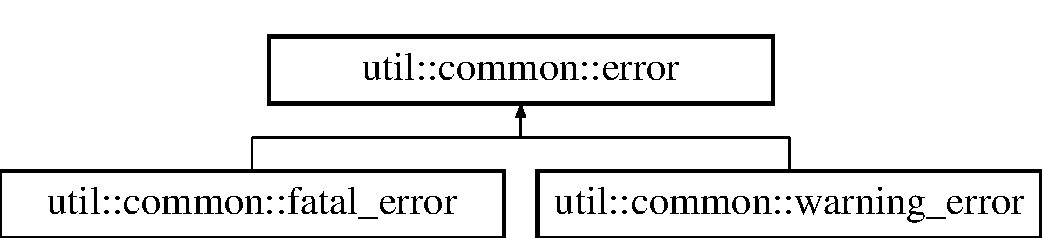
\includegraphics[height=2.000000cm]{classutil_1_1common_1_1error}
\end{center}
\end{figure}
\subsection*{\-Public \-Member \-Functions}
\begin{DoxyCompactItemize}
\item 
\hypertarget{classutil_1_1common_1_1error_afaacc98d128e170ab3f0164d62b939ed}{virtual \hyperlink{classutil_1_1common_1_1error_afaacc98d128e170ab3f0164d62b939ed}{$\sim$error} ()}\label{classutil_1_1common_1_1error_afaacc98d128e170ab3f0164d62b939ed}

\begin{DoxyCompactList}\small\item\em \-Destructor. \end{DoxyCompactList}\item 
\hypertarget{classutil_1_1common_1_1error_ad09c475e98c830b12386f14f8263927c}{virtual void \hyperlink{classutil_1_1common_1_1error_ad09c475e98c830b12386f14f8263927c}{process} () const =0}\label{classutil_1_1common_1_1error_ad09c475e98c830b12386f14f8263927c}

\begin{DoxyCompactList}\small\item\em \-Error processing method. \-See derived classes for details. \end{DoxyCompactList}\item 
\hypertarget{classutil_1_1common_1_1error_ad3395a0219f1a729d51e0a3319c348b3}{virtual \hyperlink{classutil_1_1common_1_1error_ad3395a0219f1a729d51e0a3319c348b3}{operator std\-::string} () const }\label{classutil_1_1common_1_1error_ad3395a0219f1a729d51e0a3319c348b3}

\begin{DoxyCompactList}\small\item\em \-The overloaded string type casting operator. \end{DoxyCompactList}\end{DoxyCompactItemize}
\subsection*{\-Static \-Public \-Member \-Functions}
\begin{DoxyCompactItemize}
\item 
static void \hyperlink{classutil_1_1common_1_1error_a50f2c51ec896fdd16280c5bc0b894d6c}{propogate\-\_\-error} (\hyperlink{classutil_1_1common_1_1error}{error} const $\ast$e)
\item 
static void \hyperlink{classutil_1_1common_1_1error_a110cf0bb4bff2b185d72e4a45dac21cc}{absorb\-\_\-error} (\hyperlink{classutil_1_1common_1_1error}{error} const $\ast$e)
\item 
static void \hyperlink{classutil_1_1common_1_1error_a9ba845c0e9e65f1bdba09c805f458d4e}{halt\-\_\-on\-\_\-error} (\hyperlink{classutil_1_1common_1_1error}{error} const $\ast$e)
\item 
static void \hyperlink{classutil_1_1common_1_1error_a21000e1fac6d6721d29752be0139c105}{handle\-\_\-error} (\hyperlink{classutil_1_1common_1_1error}{error} const $\ast$e)
\end{DoxyCompactItemize}
\subsection*{\-Protected \-Member \-Functions}
\begin{DoxyCompactItemize}
\item 
\hypertarget{classutil_1_1common_1_1error_a09a1f3ece8a1cfa11b6cfe808810f918}{\hyperlink{classutil_1_1common_1_1error_a09a1f3ece8a1cfa11b6cfe808810f918}{error} (char const $\ast$\-\_\-error\-\_\-msg)}\label{classutil_1_1common_1_1error_a09a1f3ece8a1cfa11b6cfe808810f918}

\begin{DoxyCompactList}\small\item\em \-Constructor. \end{DoxyCompactList}\end{DoxyCompactItemize}
\subsection*{\-Protected \-Attributes}
\begin{DoxyCompactItemize}
\item 
\hypertarget{classutil_1_1common_1_1error_a60addfad97aa8d99f59ac8bea242e548}{std\-::string \hyperlink{classutil_1_1common_1_1error_a60addfad97aa8d99f59ac8bea242e548}{error\-\_\-msg}}\label{classutil_1_1common_1_1error_a60addfad97aa8d99f59ac8bea242e548}

\begin{DoxyCompactList}\small\item\em \-The error message. \end{DoxyCompactList}\end{DoxyCompactItemize}
\subsection*{\-Friends}
\begin{DoxyCompactItemize}
\item 
\hypertarget{classutil_1_1common_1_1error_a9986db03a548ff6e2aee1541fef8b962}{std\-::ostream \& \hyperlink{classutil_1_1common_1_1error_a9986db03a548ff6e2aee1541fef8b962}{operator$<$$<$} (std\-::ostream \&str, \hyperlink{classutil_1_1common_1_1error}{error} const \&e)}\label{classutil_1_1common_1_1error_a9986db03a548ff6e2aee1541fef8b962}

\begin{DoxyCompactList}\small\item\em \-The overloaded $<$$<$ operator. \end{DoxyCompactList}\end{DoxyCompactItemize}


\subsection{\-Detailed \-Description}
\-The general error class. 

\-This is a singleton class and hence an object of this class cannot be directly instantiated. \-Only one of its derived classes can be directly instantiated. \-The class consists of the error message, a virtual general error processing method, and static error handlers. 

\subsection{\-Member \-Function \-Documentation}
\hypertarget{classutil_1_1common_1_1error_a110cf0bb4bff2b185d72e4a45dac21cc}{\index{util\-::common\-::error@{util\-::common\-::error}!absorb\-\_\-error@{absorb\-\_\-error}}
\index{absorb\-\_\-error@{absorb\-\_\-error}!util::common::error@{util\-::common\-::error}}
\subsubsection[{absorb\-\_\-error}]{\setlength{\rightskip}{0pt plus 5cm}void {\bf util\-::common\-::error\-::absorb\-\_\-error} (
\begin{DoxyParamCaption}
\item[{{\bf error} const $\ast$}]{e}
\end{DoxyParamCaption}
)\hspace{0.3cm}{\ttfamily  \mbox{[}static\mbox{]}}}}\label{classutil_1_1common_1_1error_a110cf0bb4bff2b185d72e4a45dac21cc}
\-This error handler absorbs the error and processes it as is declared in the processing method \hypertarget{classutil_1_1common_1_1error_a9ba845c0e9e65f1bdba09c805f458d4e}{\index{util\-::common\-::error@{util\-::common\-::error}!halt\-\_\-on\-\_\-error@{halt\-\_\-on\-\_\-error}}
\index{halt\-\_\-on\-\_\-error@{halt\-\_\-on\-\_\-error}!util::common::error@{util\-::common\-::error}}
\subsubsection[{halt\-\_\-on\-\_\-error}]{\setlength{\rightskip}{0pt plus 5cm}void {\bf util\-::common\-::error\-::halt\-\_\-on\-\_\-error} (
\begin{DoxyParamCaption}
\item[{{\bf error} const $\ast$}]{e}
\end{DoxyParamCaption}
)\hspace{0.3cm}{\ttfamily  \mbox{[}static\mbox{]}}}}\label{classutil_1_1common_1_1error_a9ba845c0e9e65f1bdba09c805f458d4e}
\-This error handler causes the execution to halt, irrespective of the type of the error \hypertarget{classutil_1_1common_1_1error_a21000e1fac6d6721d29752be0139c105}{\index{util\-::common\-::error@{util\-::common\-::error}!handle\-\_\-error@{handle\-\_\-error}}
\index{handle\-\_\-error@{handle\-\_\-error}!util::common::error@{util\-::common\-::error}}
\subsubsection[{handle\-\_\-error}]{\setlength{\rightskip}{0pt plus 5cm}void {\bf util\-::common\-::error\-::handle\-\_\-error} (
\begin{DoxyParamCaption}
\item[{{\bf error} const $\ast$}]{e}
\end{DoxyParamCaption}
)\hspace{0.3cm}{\ttfamily  \mbox{[}static\mbox{]}}}}\label{classutil_1_1common_1_1error_a21000e1fac6d6721d29752be0139c105}
\-This error handler propogates warning\-\_\-errors, and halts on fatal errors. \hypertarget{classutil_1_1common_1_1error_a50f2c51ec896fdd16280c5bc0b894d6c}{\index{util\-::common\-::error@{util\-::common\-::error}!propogate\-\_\-error@{propogate\-\_\-error}}
\index{propogate\-\_\-error@{propogate\-\_\-error}!util::common::error@{util\-::common\-::error}}
\subsubsection[{propogate\-\_\-error}]{\setlength{\rightskip}{0pt plus 5cm}void {\bf util\-::common\-::error\-::propogate\-\_\-error} (
\begin{DoxyParamCaption}
\item[{{\bf error} const $\ast$}]{e}
\end{DoxyParamCaption}
)\hspace{0.3cm}{\ttfamily  \mbox{[}static\mbox{]}}}}\label{classutil_1_1common_1_1error_a50f2c51ec896fdd16280c5bc0b894d6c}
\-This error handler propogates the error to the next higher level in the program hierarchy. 

\-The documentation for this class was generated from the following files\-:\begin{DoxyCompactItemize}
\item 
/home/priyanka/\-Dataset25/src/\-G\-U\-I/\hyperlink{error_8hpp}{error.\-hpp}\item 
/home/priyanka/\-Dataset25/src/\-G\-U\-I/error.\-cpp\end{DoxyCompactItemize}

\hypertarget{classFailSafe}{\section{\-Fail\-Safe \-Class \-Reference}
\label{classFailSafe}\index{\-Fail\-Safe@{\-Fail\-Safe}}
}
\subsection*{\-Public \-Member \-Functions}
\begin{DoxyCompactItemize}
\item 
\hypertarget{classFailSafe_a65aa0426223354574ed4409f139d926c}{void {\bfseries write} (\hyperlink{classScribbleArea}{\-Scribble\-Area} $\ast$\-S, string path)}\label{classFailSafe_a65aa0426223354574ed4409f139d926c}

\item 
\hypertarget{classFailSafe_afe553de2abd707c6229f73bf3a798de7}{void {\bfseries read} (\hyperlink{classScribbleArea}{\-Scribble\-Area} $\ast$\-S, string path)}\label{classFailSafe_afe553de2abd707c6229f73bf3a798de7}

\end{DoxyCompactItemize}


\-The documentation for this class was generated from the following files\-:\begin{DoxyCompactItemize}
\item 
/home/priyanka/\-Dataset25/src/\-G\-U\-I/\-Fail\-Safe.\-h\item 
/home/priyanka/\-Dataset25/src/\-G\-U\-I/\-Fail\-Safe.\-cpp\end{DoxyCompactItemize}

\hypertarget{classutil_1_1common_1_1fatal__error}{\section{util\-:\-:common\-:\-:fatal\-\_\-error \-Class \-Reference}
\label{classutil_1_1common_1_1fatal__error}\index{util\-::common\-::fatal\-\_\-error@{util\-::common\-::fatal\-\_\-error}}
}


\-The fatal error class.  




{\ttfamily \#include $<$error.\-hpp$>$}

\-Inheritance diagram for util\-:\-:common\-:\-:fatal\-\_\-error\-:\begin{figure}[H]
\begin{center}
\leavevmode
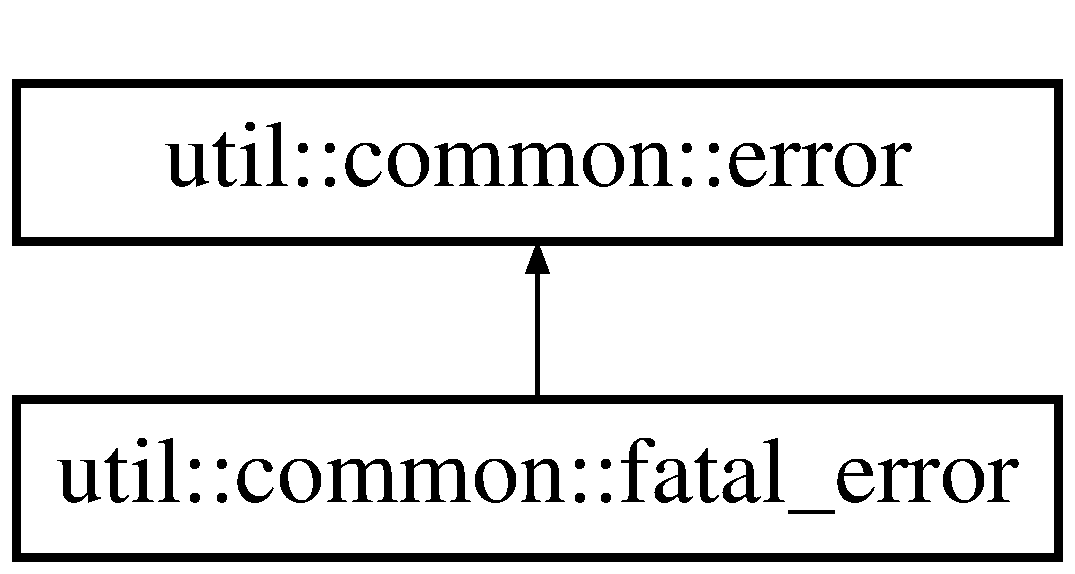
\includegraphics[height=2.000000cm]{classutil_1_1common_1_1fatal__error}
\end{center}
\end{figure}
\subsection*{\-Public \-Member \-Functions}
\begin{DoxyCompactItemize}
\item 
\hypertarget{classutil_1_1common_1_1fatal__error_a68d21d5c41478e255d0add5d20d98e13}{\hyperlink{classutil_1_1common_1_1fatal__error_a68d21d5c41478e255d0add5d20d98e13}{fatal\-\_\-error} (char const $\ast$\-\_\-error\-\_\-msg)}\label{classutil_1_1common_1_1fatal__error_a68d21d5c41478e255d0add5d20d98e13}

\begin{DoxyCompactList}\small\item\em \-Constructor. \end{DoxyCompactList}\item 
\hypertarget{classutil_1_1common_1_1fatal__error_a4066f565064ce91a317520586a2ff489}{void \hyperlink{classutil_1_1common_1_1fatal__error_a4066f565064ce91a317520586a2ff489}{process} () const }\label{classutil_1_1common_1_1fatal__error_a4066f565064ce91a317520586a2ff489}

\begin{DoxyCompactList}\small\item\em \-Error processing method. \end{DoxyCompactList}\end{DoxyCompactItemize}


\subsection{\-Detailed \-Description}
\-The fatal error class. 

\-If such an error should occur the program execution should halt 

\-The documentation for this class was generated from the following file\-:\begin{DoxyCompactItemize}
\item 
/home/priyanka/\-Dataset25/src/\-G\-U\-I/\hyperlink{error_8hpp}{error.\-hpp}\end{DoxyCompactItemize}

\hypertarget{classFrameStorage}{\section{\-Frame\-Storage \-Class \-Reference}
\label{classFrameStorage}\index{\-Frame\-Storage@{\-Frame\-Storage}}
}
\subsection*{\-Public \-Member \-Functions}
\begin{DoxyCompactItemize}
\item 
\hypertarget{classFrameStorage_aa9e09c316ad7e2496689f3751d045b75}{void {\bfseries write} (\hyperlink{classScribbleArea}{\-Scribble\-Area} $\ast$, string, int)}\label{classFrameStorage_aa9e09c316ad7e2496689f3751d045b75}

\item 
\hypertarget{classFrameStorage_a2e13939f099ca98baef14e6fe58883e5}{void {\bfseries read} (\hyperlink{classScribbleArea}{\-Scribble\-Area} $\ast$, string, int)}\label{classFrameStorage_a2e13939f099ca98baef14e6fe58883e5}

\end{DoxyCompactItemize}


\-The documentation for this class was generated from the following files\-:\begin{DoxyCompactItemize}
\item 
/home/priyanka/\-Dataset25/src/\-G\-U\-I/\-Frame\-Storage.\-h\item 
/home/priyanka/\-Dataset25/src/\-G\-U\-I/\-Frame\-Storage.\-cpp\end{DoxyCompactItemize}

\hypertarget{classGrid}{\section{\-Grid \-Class \-Reference}
\label{classGrid}\index{\-Grid@{\-Grid}}
}
\subsection*{\-Public \-Member \-Functions}
\begin{DoxyCompactItemize}
\item 
\hypertarget{classGrid_a2a809d16ae2ba160bd3a0e7a8f6406df}{{\bfseries \-Grid} (int, int)}\label{classGrid_a2a809d16ae2ba160bd3a0e7a8f6406df}

\end{DoxyCompactItemize}
\subsection*{\-Public \-Attributes}
\begin{DoxyCompactItemize}
\item 
\hypertarget{classGrid_a0c0c3a73c34785ee823cd08612efd4da}{int {\bfseries cell\-Size}}\label{classGrid_a0c0c3a73c34785ee823cd08612efd4da}

\item 
\hypertarget{classGrid_a28a6e74ffa7a0e8a2c885c269c2d1a37}{int {\bfseries cell\-Offset}}\label{classGrid_a28a6e74ffa7a0e8a2c885c269c2d1a37}

\item 
\hypertarget{classGrid_ade574c0d539d2b33b1cb57f6fd47dd2f}{vector$<$ vector$<$ \hyperlink{classCell}{\-Cell} $>$ $>$ {\bfseries cells}}\label{classGrid_ade574c0d539d2b33b1cb57f6fd47dd2f}

\end{DoxyCompactItemize}


\-The documentation for this class was generated from the following files\-:\begin{DoxyCompactItemize}
\item 
/home/priyanka/\-Dataset25/src/\-G\-U\-I/\-Grid.\-h\item 
/home/priyanka/\-Dataset25/src/\-G\-U\-I/\-Grid.\-cpp\end{DoxyCompactItemize}

\hypertarget{classHash}{\section{\-Hash \-Class \-Reference}
\label{classHash}\index{\-Hash@{\-Hash}}
}
\subsection*{\-Public \-Member \-Functions}
\begin{DoxyCompactItemize}
\item 
\hyperlink{classHash_a0d9900832f48b313f39a85866ca97e30}{\-Hash} (int x=0, int y=0, int z=0)
\begin{DoxyCompactList}\small\item\em \-Constructor1. \end{DoxyCompactList}\item 
\hyperlink{classHash_ac26af76f12633c324c56b82493bce9ef}{\-Hash} (vector$<$ vector$<$ int $>$ $>$ \&)
\begin{DoxyCompactList}\small\item\em \-Constructor2. \end{DoxyCompactList}\item 
\hypertarget{classHash_ab426e18bbe0c541990e504b1267336fe}{void \hyperlink{classHash_ab426e18bbe0c541990e504b1267336fe}{show\-Hash} ()}\label{classHash_ab426e18bbe0c541990e504b1267336fe}

\begin{DoxyCompactList}\small\item\em \-Display hash values. \end{DoxyCompactList}\item 
int \hyperlink{classHash_af1d709ab09752d4324224a4590e2d5f3}{calc\-Sketch} (vector$<$ bool $>$ \&descriptor)
\begin{DoxyCompactList}\small\item\em \-Calculate \-Sketch for a given descriptor. \end{DoxyCompactList}\end{DoxyCompactItemize}
\subsection*{\-Public \-Attributes}
\begin{DoxyCompactItemize}
\item 
vector$<$ vector$<$ int $>$ $>$ \hyperlink{classHash_a312855c01b7618ea56601216467354ee}{indices}
\begin{DoxyCompactList}\small\item\em \-Store \-Random integer values. \end{DoxyCompactList}\item 
\hypertarget{classHash_a9cf27a69da7d25a853b9b223fc189de8}{int \hyperlink{classHash_a9cf27a69da7d25a853b9b223fc189de8}{bph}}\label{classHash_a9cf27a69da7d25a853b9b223fc189de8}

\begin{DoxyCompactList}\small\item\em \hyperlink{classIndex_a32015f3d373d5ad89ec2422e6d170f26}{\-Index\-::bits\-Per\-Hash} \end{DoxyCompactList}\end{DoxyCompactItemize}


\subsection{\-Constructor \& \-Destructor \-Documentation}
\hypertarget{classHash_a0d9900832f48b313f39a85866ca97e30}{\index{\-Hash@{\-Hash}!\-Hash@{\-Hash}}
\index{\-Hash@{\-Hash}!Hash@{\-Hash}}
\subsubsection[{\-Hash}]{\setlength{\rightskip}{0pt plus 5cm}{\bf \-Hash\-::\-Hash} (
\begin{DoxyParamCaption}
\item[{int}]{x = {\ttfamily 0}, }
\item[{int}]{y = {\ttfamily 0}, }
\item[{int}]{z = {\ttfamily 0}}
\end{DoxyParamCaption}
)}}\label{classHash_a0d9900832f48b313f39a85866ca97e30}


\-Constructor1. 

\-Used when generated from code \hypertarget{classHash_ac26af76f12633c324c56b82493bce9ef}{\index{\-Hash@{\-Hash}!\-Hash@{\-Hash}}
\index{\-Hash@{\-Hash}!Hash@{\-Hash}}
\subsubsection[{\-Hash}]{\setlength{\rightskip}{0pt plus 5cm}{\bf \-Hash\-::\-Hash} (
\begin{DoxyParamCaption}
\item[{vector$<$ vector$<$ int $>$ $>$ \&}]{indices}
\end{DoxyParamCaption}
)}}\label{classHash_ac26af76f12633c324c56b82493bce9ef}


\-Constructor2. 

\-Used when already stored hash values are read from file 

\subsection{\-Member \-Function \-Documentation}
\hypertarget{classHash_af1d709ab09752d4324224a4590e2d5f3}{\index{\-Hash@{\-Hash}!calc\-Sketch@{calc\-Sketch}}
\index{calc\-Sketch@{calc\-Sketch}!Hash@{\-Hash}}
\subsubsection[{calc\-Sketch}]{\setlength{\rightskip}{0pt plus 5cm}int {\bf \-Hash\-::calc\-Sketch} (
\begin{DoxyParamCaption}
\item[{vector$<$ bool $>$ \&}]{descriptor}
\end{DoxyParamCaption}
)}}\label{classHash_af1d709ab09752d4324224a4590e2d5f3}


\-Calculate \-Sketch for a given descriptor. 

\-Will apply hash function to descriptor provided as input i.\-e. permute the binary descriptor using indices\mbox{[}i\mbox{]} and search for the lowest index containing 1. \-This is done for all hash functions stored in /ref \hyperlink{classHash_a312855c01b7618ea56601216467354ee}{\-Hash\-::indices} and concatenated together to generate final sketch. 

\subsection{\-Member \-Data \-Documentation}
\hypertarget{classHash_a312855c01b7618ea56601216467354ee}{\index{\-Hash@{\-Hash}!indices@{indices}}
\index{indices@{indices}!Hash@{\-Hash}}
\subsubsection[{indices}]{\setlength{\rightskip}{0pt plus 5cm}vector$<$vector$<$int$>$ $>$ {\bf \-Hash\-::indices}}}\label{classHash_a312855c01b7618ea56601216467354ee}


\-Store \-Random integer values. 

\-It will store random integer values within the range of 0 to max descriptor size to permute the index of binary descriptor. \-Second index consist of hash function. \-First index denotes total number of hash function needed to generate sketch. 

\-The documentation for this class was generated from the following files\-:\begin{DoxyCompactItemize}
\item 
/home/priyanka/\-Dataset25/src/db/\hyperlink{Hash_8h}{\-Hash.\-h}\item 
/home/priyanka/\-Dataset25/src/db/\-Hash.\-cpp\end{DoxyCompactItemize}

\hypertarget{classHasher}{\section{\-Hasher \-Class \-Reference}
\label{classHasher}\index{\-Hasher@{\-Hasher}}
}
\subsection*{\-Public \-Member \-Functions}
\begin{DoxyCompactItemize}
\item 
\hypertarget{classHasher_a6f581218408d8422c49b6109cc6197af}{size\-\_\-t \hyperlink{classHasher_a6f581218408d8422c49b6109cc6197af}{operator()} (\hyperlink{classEntry}{\-Entry} const \&key) const }\label{classHasher_a6f581218408d8422c49b6109cc6197af}

\begin{DoxyCompactList}\small\item\em \-Helper class for \-Resut\-Set\-::m. \end{DoxyCompactList}\end{DoxyCompactItemize}


\-The documentation for this class was generated from the following file\-:\begin{DoxyCompactItemize}
\item 
/home/priyanka/\-Dataset25/src/db/\hyperlink{ResultSet_8h}{\-Result\-Set.\-h}\end{DoxyCompactItemize}

\hypertarget{classHistogram}{\section{\-Histogram \-Class \-Reference}
\label{classHistogram}\index{\-Histogram@{\-Histogram}}
}
\subsection*{\-Public \-Member \-Functions}
\begin{DoxyCompactItemize}
\item 
\hypertarget{classHistogram_ad28261323845d54ecd0d0218e7942f1f}{\hyperlink{classHistogram_ad28261323845d54ecd0d0218e7942f1f}{\-Histogram} (double, double, int, double, double, int, double, double, int)}\label{classHistogram_ad28261323845d54ecd0d0218e7942f1f}

\begin{DoxyCompactList}\small\item\em \-Constructor. \end{DoxyCompactList}\item 
void \hyperlink{classHistogram_a8bdace3d883806855fb401b4ed1ebeed}{increment} (double, double, double, double)
\begin{DoxyCompactList}\small\item\em \-Will increment the histogram value on the basis of normalized magnitude of pixel. \end{DoxyCompactList}\item 
\hypertarget{classHistogram_a9423dec20de4a1034360e813656c44c1}{void \hyperlink{classHistogram_a9423dec20de4a1034360e813656c44c1}{show} ()}\label{classHistogram_a9423dec20de4a1034360e813656c44c1}

\begin{DoxyCompactList}\small\item\em \-Shows the histogram for a patch in all orientation in image form. \end{DoxyCompactList}\item 
\hypertarget{classHistogram_aa1bdca4cadfc0b6e2810ea95379dac3e}{void \hyperlink{classHistogram_aa1bdca4cadfc0b6e2810ea95379dac3e}{blur} (int, int)}\label{classHistogram_aa1bdca4cadfc0b6e2810ea95379dac3e}

\begin{DoxyCompactList}\small\item\em \-Blur the histogram to provide robustness. \end{DoxyCompactList}\item 
\hypertarget{classHistogram_ab0eb6d0a65594891669eb4b76dc842d7}{double \hyperlink{classHistogram_ab0eb6d0a65594891669eb4b76dc842d7}{interpolate} (double, double, double)}\label{classHistogram_ab0eb6d0a65594891669eb4b76dc842d7}

\begin{DoxyCompactList}\small\item\em \-Function will return interpolated value. \end{DoxyCompactList}\item 
\hypertarget{classHistogram_a2be8d28fd551e3c2093a4d2069c8a6fa}{double \hyperlink{classHistogram_a2be8d28fd551e3c2093a4d2069c8a6fa}{b\-Final\-Value} (double, double, double)}\label{classHistogram_a2be8d28fd551e3c2093a4d2069c8a6fa}

\begin{DoxyCompactList}\small\item\em \-Will perform 3\-D interpolation using \-Histogram\-:\-: \hyperlink{classHistogram_ab0eb6d0a65594891669eb4b76dc842d7}{interpolate(double,double,double)} function. \end{DoxyCompactList}\item 
void \hyperlink{classHistogram_af415436ff0dc65684d0f48cfdff11863}{resample} (int, int, int, vector$<$ double $>$ \&)
\begin{DoxyCompactList}\small\item\em \-Resample the histogram value to reduce its size. \end{DoxyCompactList}\end{DoxyCompactItemize}


\subsection{\-Member \-Function \-Documentation}
\hypertarget{classHistogram_a8bdace3d883806855fb401b4ed1ebeed}{\index{\-Histogram@{\-Histogram}!increment@{increment}}
\index{increment@{increment}!Histogram@{\-Histogram}}
\subsubsection[{increment}]{\setlength{\rightskip}{0pt plus 5cm}void {\bf \-Histogram\-::increment} (
\begin{DoxyParamCaption}
\item[{double}]{x, }
\item[{double}]{y, }
\item[{double}]{t, }
\item[{double}]{nor\-Magnitude}
\end{DoxyParamCaption}
)}}\label{classHistogram_a8bdace3d883806855fb401b4ed1ebeed}


\-Will increment the histogram value on the basis of normalized magnitude of pixel. 

\-It will first calculate the bins in which the pixel location and orientation fall and then using bilinear interpolation it add values to all the bins nearest to the calculated bin \hypertarget{classHistogram_af415436ff0dc65684d0f48cfdff11863}{\index{\-Histogram@{\-Histogram}!resample@{resample}}
\index{resample@{resample}!Histogram@{\-Histogram}}
\subsubsection[{resample}]{\setlength{\rightskip}{0pt plus 5cm}void {\bf \-Histogram\-::resample} (
\begin{DoxyParamCaption}
\item[{int}]{xbuck2, }
\item[{int}]{ybuck2, }
\item[{int}]{tbuck2, }
\item[{vector$<$ double $>$ \&}]{vals}
\end{DoxyParamCaption}
)}}\label{classHistogram_af415436ff0dc65684d0f48cfdff11863}


\-Resample the histogram value to reduce its size. 

\-Instead of taking histogram values at all the bins, histogram values are taken at some sample bins. \-If the sample bins are at some intermediate values then using interpolatioin, values from neighboring bins are stored in the sample bin. 

\-The documentation for this class was generated from the following files\-:\begin{DoxyCompactItemize}
\item 
/home/priyanka/\-Dataset25/src/\-G\-U\-I/\hyperlink{Histogram_8h}{\-Histogram.\-h}\item 
/home/priyanka/\-Dataset25/src/\-G\-U\-I/\-Histogram.\-cpp\end{DoxyCompactItemize}

\hypertarget{classImageVotes}{\section{\-Image\-Votes \-Class \-Reference}
\label{classImageVotes}\index{\-Image\-Votes@{\-Image\-Votes}}
}
\subsection*{\-Public \-Member \-Functions}
\begin{DoxyCompactItemize}
\item 
\hypertarget{classImageVotes_ad4607ac8f62f3fcf496b4a121a00ee4a}{{\bfseries \-Image\-Votes} (int img\-Id, \hyperlink{classGrid}{\-Grid} grid)}\label{classImageVotes_ad4607ac8f62f3fcf496b4a121a00ee4a}

\item 
\hypertarget{classImageVotes_aca051dafc2593acf206982ccba89f29e}{int {\bfseries alter\-Votes} (int, int, int)}\label{classImageVotes_aca051dafc2593acf206982ccba89f29e}

\end{DoxyCompactItemize}
\subsection*{\-Public \-Attributes}
\begin{DoxyCompactItemize}
\item 
\hypertarget{classImageVotes_ab091b6fc057a340e0dec1ec8ecdc2068}{int {\bfseries offset\-Size}}\label{classImageVotes_ab091b6fc057a340e0dec1ec8ecdc2068}

\item 
\hypertarget{classImageVotes_ae5270d0d4b6f9ae069b3cb926bd29c0e}{int {\bfseries img\-Id}}\label{classImageVotes_ae5270d0d4b6f9ae069b3cb926bd29c0e}

\item 
\hypertarget{classImageVotes_a244e45706478d62a53b13db049b47b52}{\hyperlink{classGrid}{\-Grid} {\bfseries grid}}\label{classImageVotes_a244e45706478d62a53b13db049b47b52}

\item 
\hypertarget{classImageVotes_a6db69485a42c5fae731e4800b08a5b26}{vector$<$ vector$<$ int $>$ $>$ {\bfseries offsets}}\label{classImageVotes_a6db69485a42c5fae731e4800b08a5b26}

\item 
\hypertarget{classImageVotes_a63af62d90937f1f65c6c6bf6ea071c5f}{int {\bfseries max\-Votes}}\label{classImageVotes_a63af62d90937f1f65c6c6bf6ea071c5f}

\item 
\hypertarget{classImageVotes_abf09b33968b11ab551f472ad16eab411}{int {\bfseries maxbin\-X}}\label{classImageVotes_abf09b33968b11ab551f472ad16eab411}

\item 
\hypertarget{classImageVotes_aa7286de7d363910a712f1ff6312709c0}{int {\bfseries maxbin\-Y}}\label{classImageVotes_aa7286de7d363910a712f1ff6312709c0}

\end{DoxyCompactItemize}


\-The documentation for this class was generated from the following files\-:\begin{DoxyCompactItemize}
\item 
/home/priyanka/\-Dataset25/src/\-G\-U\-I/\-Image\-Votes.\-h\item 
/home/priyanka/\-Dataset25/src/\-G\-U\-I/\-Image\-Votes.\-cpp\end{DoxyCompactItemize}

\hypertarget{classIndex}{\section{\-Index \-Class \-Reference}
\label{classIndex}\index{\-Index@{\-Index}}
}
\subsection*{\-Public \-Member \-Functions}
\begin{DoxyCompactItemize}
\item 
\hypertarget{classIndex_a25ad808f35997941d138c5b1e7cde441}{\hyperlink{classIndex_a25ad808f35997941d138c5b1e7cde441}{\-Index} (int=0, int=0, int=0)}\label{classIndex_a25ad808f35997941d138c5b1e7cde441}

\begin{DoxyCompactList}\small\item\em \-Constructor. \end{DoxyCompactList}\item 
void \hyperlink{classIndex_ad4569374473db6e4180e7f5e5cbe1cf6}{generate\-Hashes} ()
\item 
\hypertarget{classIndex_a98ce1753ab600b67d85dae0b01020b0d}{void \hyperlink{classIndex_a98ce1753ab600b67d85dae0b01020b0d}{reverse\-Index} ()}\label{classIndex_a98ce1753ab600b67d85dae0b01020b0d}

\begin{DoxyCompactList}\small\item\em \-Call \-:\-: \hyperlink{classIndex_a98ce1753ab600b67d85dae0b01020b0d}{reverse\-Index()} function to generate all the sketches for a descriptor. \end{DoxyCompactList}\item 
\hypertarget{classIndex_a3132e2144d7549df4697db885be653e3}{void \hyperlink{classIndex_a3132e2144d7549df4697db885be653e3}{fill\-Entry} (vector$<$ bool $>$ \&, int, int, int)}\label{classIndex_a3132e2144d7549df4697db885be653e3}

\begin{DoxyCompactList}\small\item\em \-Call \-:\-: \hyperlink{classIndex_a3132e2144d7549df4697db885be653e3}{fill\-Entry()} function to generate all the sketches for a descriptor. \end{DoxyCompactList}\item 
\hyperlink{classResultSet}{\-Result\-Set} $\ast$ \hyperlink{classIndex_a7d5c9e47037fc4685fc71acab1544b43}{find\-All\-Entries} (vector$<$ bool $>$ \&)
\item 
\hypertarget{classIndex_aa9c882998bed9437303b41b377ccc330}{\hyperlink{classResultSet}{\-Result\-Set} $\ast$ {\bfseries find\-Entries} (vector$<$ bool $>$ \&, int)}\label{classIndex_aa9c882998bed9437303b41b377ccc330}

\end{DoxyCompactItemize}
\subsection*{\-Public \-Attributes}
\begin{DoxyCompactItemize}
\item 
\hypertarget{classIndex_af70cace4ee2df00ea9f3abbdd4a03e31}{int \hyperlink{classIndex_af70cace4ee2df00ea9f3abbdd4a03e31}{total\-\_\-sketch}}\label{classIndex_af70cace4ee2df00ea9f3abbdd4a03e31}

\begin{DoxyCompactList}\small\item\em \-Total no. of sketch per patch. \end{DoxyCompactList}\item 
\hypertarget{classIndex_a7e25594ed3a2d5af48a3370c36ac6481}{int \hyperlink{classIndex_a7e25594ed3a2d5af48a3370c36ac6481}{total\-\_\-hashf}}\label{classIndex_a7e25594ed3a2d5af48a3370c36ac6481}

\begin{DoxyCompactList}\small\item\em \-Total min hash functions used to generate sketch. \end{DoxyCompactList}\item 
int \hyperlink{classIndex_a32015f3d373d5ad89ec2422e6d170f26}{bits\-Per\-Hash}
\begin{DoxyCompactList}\small\item\em \-Number of bits required to denote the maximum index in binary descriptor. \end{DoxyCompactList}\item 
int \hyperlink{classIndex_ac11c8f73f786ae87d455b214d6978fd1}{\-Descriptorbits}
\begin{DoxyCompactList}\small\item\em \-Number of bits per hash value. \end{DoxyCompactList}\item 
vector$<$ string $>$ \hyperlink{classIndex_a10d91af933c37e605b1d9bd1a3995f8c}{image\-Names}
\begin{DoxyCompactList}\small\item\em \-Its consist of image names of all the images in database. \end{DoxyCompactList}\item 
\hypertarget{classIndex_a3ad2c35848d27fa5a49b78bece15902f}{vector$<$ \hyperlink{classTable}{\-Table} $>$ \hyperlink{classIndex_a3ad2c35848d27fa5a49b78bece15902f}{tables}}\label{classIndex_a3ad2c35848d27fa5a49b78bece15902f}

\begin{DoxyCompactList}\small\item\em \-Data struture to hold all the hash function generated using \-Index\-:\-: generate\-Hashesh() function. \end{DoxyCompactList}\end{DoxyCompactItemize}


\subsection{\-Member \-Function \-Documentation}
\hypertarget{classIndex_a7d5c9e47037fc4685fc71acab1544b43}{\index{\-Index@{\-Index}!find\-All\-Entries@{find\-All\-Entries}}
\index{find\-All\-Entries@{find\-All\-Entries}!Index@{\-Index}}
\subsubsection[{find\-All\-Entries}]{\setlength{\rightskip}{0pt plus 5cm}{\bf \-Result\-Set} $\ast$ {\bf \-Index\-::find\-All\-Entries} (
\begin{DoxyParamCaption}
\item[{vector$<$ bool $>$ \&}]{descriptor}
\end{DoxyParamCaption}
)}}\label{classIndex_a7d5c9e47037fc4685fc71acab1544b43}
\-Take descriptor and will generate all the entries that will be produced for given descriptor by applying different hash function stored in different \-Table\-::table \hypertarget{classIndex_ad4569374473db6e4180e7f5e5cbe1cf6}{\index{\-Index@{\-Index}!generate\-Hashes@{generate\-Hashes}}
\index{generate\-Hashes@{generate\-Hashes}!Index@{\-Index}}
\subsubsection[{generate\-Hashes}]{\setlength{\rightskip}{0pt plus 5cm}void {\bf \-Index\-::generate\-Hashes} (
\begin{DoxyParamCaption}
{}
\end{DoxyParamCaption}
)}}\label{classIndex_ad4569374473db6e4180e7f5e5cbe1cf6}
\-Generate \hyperlink{classIndex_af70cace4ee2df00ea9f3abbdd4a03e31}{\-Index\-::total\-\_\-sketch} number of different \hyperlink{classIndex_a7e25594ed3a2d5af48a3370c36ac6481}{\-Index\-::total\-\_\-hashf} set of min hash function. \-These hash functions are stored in \hyperlink{classTable}{\-Table} 

\subsection{\-Member \-Data \-Documentation}
\hypertarget{classIndex_a32015f3d373d5ad89ec2422e6d170f26}{\index{\-Index@{\-Index}!bits\-Per\-Hash@{bits\-Per\-Hash}}
\index{bits\-Per\-Hash@{bits\-Per\-Hash}!Index@{\-Index}}
\subsubsection[{bits\-Per\-Hash}]{\setlength{\rightskip}{0pt plus 5cm}int {\bf \-Index\-::bits\-Per\-Hash}}}\label{classIndex_a32015f3d373d5ad89ec2422e6d170f26}


\-Number of bits required to denote the maximum index in binary descriptor. 

\hyperlink{classIndex_a7e25594ed3a2d5af48a3370c36ac6481}{\-Index\-::total\-\_\-hashf} are used to calculate the min hash value which is the smallest index containing 1 after permuting the binary descriptor. \-These min hash values bits are concatenated together to find the final sketch. \-To concatenate them bits its required to get the maximum number of bits required to denote the hash value. \-And max hash value can be the last index of the descriptor, hence its log\-\_\-2 of size of descriptor \hypertarget{classIndex_ac11c8f73f786ae87d455b214d6978fd1}{\index{\-Index@{\-Index}!\-Descriptorbits@{\-Descriptorbits}}
\index{\-Descriptorbits@{\-Descriptorbits}!Index@{\-Index}}
\subsubsection[{\-Descriptorbits}]{\setlength{\rightskip}{0pt plus 5cm}int {\bf \-Index\-::\-Descriptorbits}}}\label{classIndex_ac11c8f73f786ae87d455b214d6978fd1}


\-Number of bits per hash value. 

\-Since histogram is converted to binary hash, size of histogram is equivalent to bits\-Per\-Hash. \hypertarget{classIndex_a10d91af933c37e605b1d9bd1a3995f8c}{\index{\-Index@{\-Index}!image\-Names@{image\-Names}}
\index{image\-Names@{image\-Names}!Index@{\-Index}}
\subsubsection[{image\-Names}]{\setlength{\rightskip}{0pt plus 5cm}vector$<$string$>$ {\bf \-Index\-::image\-Names}}}\label{classIndex_a10d91af933c37e605b1d9bd1a3995f8c}


\-Its consist of image names of all the images in database. 

\-This will be used later to retrieve the image from database. 

\-The documentation for this class was generated from the following files\-:\begin{DoxyCompactItemize}
\item 
/home/priyanka/\-Dataset25/src/db/\hyperlink{Index_8h}{\-Index.\-h}\item 
/home/priyanka/\-Dataset25/src/db/\-Index.\-cpp\end{DoxyCompactItemize}

\hypertarget{classIndexStorage}{\section{\-Index\-Storage \-Class \-Reference}
\label{classIndexStorage}\index{\-Index\-Storage@{\-Index\-Storage}}
}
\subsection*{\-Public \-Member \-Functions}
\begin{DoxyCompactItemize}
\item 
\hypertarget{classIndexStorage_a6bae45234b690eb9ffca45b3033de28a}{void {\bfseries write} (string, \hyperlink{classIndex}{\-Index}, string)}\label{classIndexStorage_a6bae45234b690eb9ffca45b3033de28a}

\item 
\hypertarget{classIndexStorage_adfb66513f7c684d6df29d73f92f62a9c}{\hyperlink{classIndex}{\-Index} {\bfseries read} (string)}\label{classIndexStorage_adfb66513f7c684d6df29d73f92f62a9c}

\end{DoxyCompactItemize}


\-The documentation for this class was generated from the following files\-:\begin{DoxyCompactItemize}
\item 
/home/priyanka/\-Dataset25/src/\-G\-U\-I/\-Index\-Storage.\-h\item 
/home/priyanka/\-Dataset25/src/\-G\-U\-I/\-Index\-Storage.\-cpp\end{DoxyCompactItemize}

\hypertarget{classMainWindow}{\section{\-Main\-Window \-Class \-Reference}
\label{classMainWindow}\index{\-Main\-Window@{\-Main\-Window}}
}
\subsection*{\-Public \-Attributes}
\begin{DoxyCompactItemize}
\item 
\hypertarget{classMainWindow_af4e870742baec6e7da3d263501160123}{\hyperlink{classFrameStorage}{\-Frame\-Storage} {\bfseries f\-S}}\label{classMainWindow_af4e870742baec6e7da3d263501160123}

\item 
\hypertarget{classMainWindow_ac1c375e813f0acfd9bd2075f8e53b7bf}{\hyperlink{classFailSafe}{\-Fail\-Safe} {\bfseries failsafe}}\label{classMainWindow_ac1c375e813f0acfd9bd2075f8e53b7bf}

\item 
\hypertarget{classMainWindow_ac1dfe6d34127a7bfb21ff68302ac6b7b}{int {\bfseries frame\-\_\-no}}\label{classMainWindow_ac1dfe6d34127a7bfb21ff68302ac6b7b}

\item 
\hypertarget{classMainWindow_a3d02064c7363d879739b53077ddff72b}{int {\bfseries frame\-\_\-drawn}}\label{classMainWindow_a3d02064c7363d879739b53077ddff72b}

\item 
\hypertarget{classMainWindow_aa98a0ff34380a1f5f3f84f400eca4c56}{int {\bfseries play\-\_\-frame}}\label{classMainWindow_aa98a0ff34380a1f5f3f84f400eca4c56}

\end{DoxyCompactItemize}


\-The documentation for this class was generated from the following files\-:\begin{DoxyCompactItemize}
\item 
/home/priyanka/\-Dataset25/src/\-G\-U\-I/mainwindow.\-h\item 
/home/priyanka/\-Dataset25/src/\-G\-U\-I/mainwindow.\-cpp\end{DoxyCompactItemize}

\hypertarget{classUi_1_1MainWindow}{\section{\-Ui\-:\-:\-Main\-Window \-Class \-Reference}
\label{classUi_1_1MainWindow}\index{\-Ui\-::\-Main\-Window@{\-Ui\-::\-Main\-Window}}
}
\-Inheritance diagram for \-Ui\-:\-:\-Main\-Window\-:\begin{figure}[H]
\begin{center}
\leavevmode
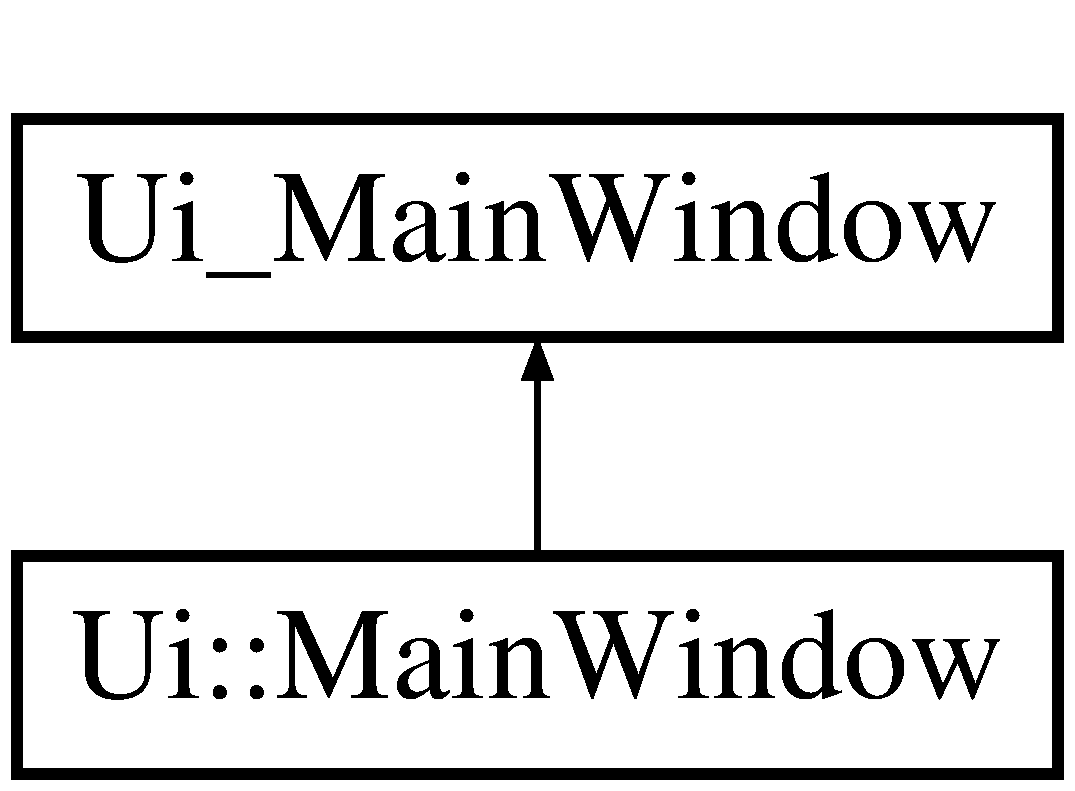
\includegraphics[height=2.000000cm]{classUi_1_1MainWindow}
\end{center}
\end{figure}


\-The documentation for this class was generated from the following file\-:\begin{DoxyCompactItemize}
\item 
/home/priyanka/\-Dataset25/src/\-G\-U\-I/ui\-\_\-mainwindow.\-h\end{DoxyCompactItemize}

\hypertarget{classutil_1_1math_1_1mat33}{\section{util\-:\-:math\-:\-:mat33 \-Class \-Reference}
\label{classutil_1_1math_1_1mat33}\index{util\-::math\-::mat33@{util\-::math\-::mat33}}
}


\-This is a general 3x3 matrix class.  




{\ttfamily \#include $<$matvec.\-hpp$>$}

\subsection*{\-Public \-Member \-Functions}
\begin{DoxyCompactItemize}
\item 
\hypertarget{classutil_1_1math_1_1mat33_a833247977b36449f4d7a608131aeedb3}{\hyperlink{classutil_1_1math_1_1mat33_a833247977b36449f4d7a608131aeedb3}{$\sim$mat33} ()}\label{classutil_1_1math_1_1mat33_a833247977b36449f4d7a608131aeedb3}

\begin{DoxyCompactList}\small\item\em \-Destructor. \end{DoxyCompactList}\item 
\hypertarget{classutil_1_1math_1_1mat33_aae87588948ff698c5b9b0c4d33274aac}{\hyperlink{classutil_1_1math_1_1vec3}{vec3} \& \hyperlink{classutil_1_1math_1_1mat33_aae87588948ff698c5b9b0c4d33274aac}{operator\mbox{[}$\,$\mbox{]}} (int index)}\label{classutil_1_1math_1_1mat33_aae87588948ff698c5b9b0c4d33274aac}

\begin{DoxyCompactList}\small\item\em \-Overloaded \mbox{[}\mbox{]} operator. \end{DoxyCompactList}\item 
\hypertarget{classutil_1_1math_1_1mat33_adbeb70a11f8184d4a74731e3712d7460}{\hyperlink{classutil_1_1math_1_1vec3}{vec3} \hyperlink{classutil_1_1math_1_1mat33_adbeb70a11f8184d4a74731e3712d7460}{operator\mbox{[}$\,$\mbox{]}} (int index) const }\label{classutil_1_1math_1_1mat33_adbeb70a11f8184d4a74731e3712d7460}

\begin{DoxyCompactList}\small\item\em \-Overloaded \mbox{[}\mbox{]} operator. \end{DoxyCompactList}\item 
\hypertarget{classutil_1_1math_1_1mat33_a4e5702e23061356eeb8272478fe092f7}{\hyperlink{classutil_1_1math_1_1mat33}{mat33} \hyperlink{classutil_1_1math_1_1mat33_a4e5702e23061356eeb8272478fe092f7}{transpose} (void)}\label{classutil_1_1math_1_1mat33_a4e5702e23061356eeb8272478fe092f7}

\begin{DoxyCompactList}\small\item\em \-Returns the transpose of the matrix. \end{DoxyCompactList}\item 
\hypertarget{classutil_1_1math_1_1mat33_a8e8805ded1df790e903db5dbb2fad1e8}{\hyperlink{classutil_1_1math_1_1mat33}{mat33} \hyperlink{classutil_1_1math_1_1mat33_a8e8805ded1df790e903db5dbb2fad1e8}{inverse} (void)}\label{classutil_1_1math_1_1mat33_a8e8805ded1df790e903db5dbb2fad1e8}

\begin{DoxyCompactList}\small\item\em \-Returns the inverse of the matrix. \end{DoxyCompactList}\item 
\hypertarget{classutil_1_1math_1_1mat33_a8da8164e4b80b47c8e039d7b9d2bbc50}{\hyperlink{classutil_1_1math_1_1mat33}{mat33} \& \hyperlink{classutil_1_1math_1_1mat33_a8da8164e4b80b47c8e039d7b9d2bbc50}{map} (double($\ast$fn)(double))}\label{classutil_1_1math_1_1mat33_a8da8164e4b80b47c8e039d7b9d2bbc50}

\begin{DoxyCompactList}\small\item\em \-Maps the function to every element of the matrix. \end{DoxyCompactList}\item 
\hypertarget{classutil_1_1math_1_1mat33_a609b696742eb3871ccd570b788688e0a}{void \hyperlink{classutil_1_1math_1_1mat33_a609b696742eb3871ccd570b788688e0a}{set} (const \hyperlink{classutil_1_1math_1_1vec3}{vec3} \&v0, const \hyperlink{classutil_1_1math_1_1vec3}{vec3} \&v1, const \hyperlink{classutil_1_1math_1_1vec3}{vec3} \&v2)}\label{classutil_1_1math_1_1mat33_a609b696742eb3871ccd570b788688e0a}

\begin{DoxyCompactList}\small\item\em \-Sets the value of the matrix. \end{DoxyCompactList}\item 
\hypertarget{classutil_1_1math_1_1mat33_af87b9f7e3cf37af7305b0272ad027533}{void \hyperlink{classutil_1_1math_1_1mat33_af87b9f7e3cf37af7305b0272ad027533}{set} (double arr\mbox{[}3\mbox{]}\mbox{[}3\mbox{]})}\label{classutil_1_1math_1_1mat33_af87b9f7e3cf37af7305b0272ad027533}

\begin{DoxyCompactList}\small\item\em \-Sets the value of the matrix. \end{DoxyCompactList}\item 
\hypertarget{classutil_1_1math_1_1mat33_aa9e09b285f5c7adcb98aec887d6edbdf}{void \hyperlink{classutil_1_1math_1_1mat33_aa9e09b285f5c7adcb98aec887d6edbdf}{print} (\-F\-I\-L\-E $\ast$file, std\-::string name)}\label{classutil_1_1math_1_1mat33_aa9e09b285f5c7adcb98aec887d6edbdf}

\begin{DoxyCompactList}\small\item\em \-Print the matrix to a file. \end{DoxyCompactList}\item 
\hypertarget{classutil_1_1math_1_1mat33_aa40827034ad16f60f2268645ad4035d9}{void \hyperlink{classutil_1_1math_1_1mat33_aa40827034ad16f60f2268645ad4035d9}{swap\-\_\-rows} (int i, int j)}\label{classutil_1_1math_1_1mat33_aa40827034ad16f60f2268645ad4035d9}

\begin{DoxyCompactList}\small\item\em \-Swap rows i and j. \end{DoxyCompactList}\item 
\hypertarget{classutil_1_1math_1_1mat33_a3ac6b654e27e0f2a4a5dc741f264d7f2}{void \hyperlink{classutil_1_1math_1_1mat33_a3ac6b654e27e0f2a4a5dc741f264d7f2}{swap\-\_\-cols} (int i, int j)}\label{classutil_1_1math_1_1mat33_a3ac6b654e27e0f2a4a5dc741f264d7f2}

\begin{DoxyCompactList}\small\item\em \-Swap columns i and j. \end{DoxyCompactList}\end{DoxyCompactItemize}
{\bf }\par
\begin{DoxyCompactItemize}
\item 
\hypertarget{classutil_1_1math_1_1mat33_a403a6779d3b01de177e57d47c1d979f3}{\hyperlink{classutil_1_1math_1_1mat33_a403a6779d3b01de177e57d47c1d979f3}{mat33} ()}\label{classutil_1_1math_1_1mat33_a403a6779d3b01de177e57d47c1d979f3}

\begin{DoxyCompactList}\small\item\em \-Constructor. \end{DoxyCompactList}\item 
\hypertarget{classutil_1_1math_1_1mat33_ab8e7b9217a0d8c0b9b179c44d3910851}{{\bfseries mat33} (const \hyperlink{classutil_1_1math_1_1vec3}{vec3} \&v1, const \hyperlink{classutil_1_1math_1_1vec3}{vec3} \&v2, const \hyperlink{classutil_1_1math_1_1vec3}{vec3} \&v3)}\label{classutil_1_1math_1_1mat33_ab8e7b9217a0d8c0b9b179c44d3910851}

\item 
\hypertarget{classutil_1_1math_1_1mat33_af61293c06efdb5e74ee9c224a68cd64c}{{\bfseries mat33} (const double d)}\label{classutil_1_1math_1_1mat33_af61293c06efdb5e74ee9c224a68cd64c}

\item 
\hypertarget{classutil_1_1math_1_1mat33_abe5a196ee8a813766123e5614eff325c}{{\bfseries mat33} (const \hyperlink{classutil_1_1math_1_1mat33}{mat33} \&m)}\label{classutil_1_1math_1_1mat33_abe5a196ee8a813766123e5614eff325c}

\item 
\hypertarget{classutil_1_1math_1_1mat33_a04df60084c74336543ece5286a093751}{{\bfseries mat33} (const double a00, const double a01, const double a02, const double a10, const double a11, const double a12, const double a20, const double a21, const double a22)}\label{classutil_1_1math_1_1mat33_a04df60084c74336543ece5286a093751}

\item 
\hypertarget{classutil_1_1math_1_1mat33_a84c33565f35fc3ab5bef208c3acdc9e0}{{\bfseries mat33} (const double a\mbox{[}3\mbox{]}\mbox{[}3\mbox{]})}\label{classutil_1_1math_1_1mat33_a84c33565f35fc3ab5bef208c3acdc9e0}

\end{DoxyCompactItemize}

{\bf }\par
\begin{DoxyCompactItemize}
\item 
\hypertarget{classutil_1_1math_1_1mat33_aabda4867fd839281bac9b2bea1d98ca3}{\hyperlink{classutil_1_1math_1_1mat33}{mat33} \& \hyperlink{classutil_1_1math_1_1mat33_aabda4867fd839281bac9b2bea1d98ca3}{operator=} (const \hyperlink{classutil_1_1math_1_1mat33}{mat33} \&m)}\label{classutil_1_1math_1_1mat33_aabda4867fd839281bac9b2bea1d98ca3}

\begin{DoxyCompactList}\small\item\em \-Overloaded assignment operators. \end{DoxyCompactList}\item 
\hypertarget{classutil_1_1math_1_1mat33_a8bc0ae6905d964e0d6cadbb037eff301}{\hyperlink{classutil_1_1math_1_1mat33}{mat33} \& {\bfseries operator+=} (const \hyperlink{classutil_1_1math_1_1mat33}{mat33} \&m)}\label{classutil_1_1math_1_1mat33_a8bc0ae6905d964e0d6cadbb037eff301}

\item 
\hypertarget{classutil_1_1math_1_1mat33_a306ed83171f265ce9f9d822b4135a3a3}{\hyperlink{classutil_1_1math_1_1mat33}{mat33} \& {\bfseries operator-\/=} (const \hyperlink{classutil_1_1math_1_1mat33}{mat33} \&m)}\label{classutil_1_1math_1_1mat33_a306ed83171f265ce9f9d822b4135a3a3}

\item 
\hypertarget{classutil_1_1math_1_1mat33_a6440c3127d4fb5a3f3eeb40fbb06a7bb}{\hyperlink{classutil_1_1math_1_1mat33}{mat33} \& {\bfseries operator$\ast$=} (const double d)}\label{classutil_1_1math_1_1mat33_a6440c3127d4fb5a3f3eeb40fbb06a7bb}

\item 
\hypertarget{classutil_1_1math_1_1mat33_a67b436c8767e3d49f338dae202585c02}{\hyperlink{classutil_1_1math_1_1mat33}{mat33} \& {\bfseries operator/=} (const double d)}\label{classutil_1_1math_1_1mat33_a67b436c8767e3d49f338dae202585c02}

\end{DoxyCompactItemize}

\subsection*{\-Static \-Public \-Member \-Functions}
\begin{DoxyCompactItemize}
\item 
\hypertarget{classutil_1_1math_1_1mat33_afc887f0aa54e0b159a2c4993a19fdf36}{static \hyperlink{classutil_1_1math_1_1mat33}{mat33} \hyperlink{classutil_1_1math_1_1mat33_afc887f0aa54e0b159a2c4993a19fdf36}{identity2\-D} (void)}\label{classutil_1_1math_1_1mat33_afc887f0aa54e0b159a2c4993a19fdf36}

\begin{DoxyCompactList}\small\item\em 2\-D identity matrix \end{DoxyCompactList}\item 
\hypertarget{classutil_1_1math_1_1mat33_aebca188a2f554b0799dff8f2fc0d72e4}{static \hyperlink{classutil_1_1math_1_1mat33}{mat33} \hyperlink{classutil_1_1math_1_1mat33_aebca188a2f554b0799dff8f2fc0d72e4}{rotation2\-D} (\hyperlink{classutil_1_1math_1_1vec2}{vec2} \&center, double theta)}\label{classutil_1_1math_1_1mat33_aebca188a2f554b0799dff8f2fc0d72e4}

\begin{DoxyCompactList}\small\item\em 2\-D rotation matrix (postmultiply column vector) \end{DoxyCompactList}\item 
\hypertarget{classutil_1_1math_1_1mat33_abf6f4e4217c5c86d1c83ee6e1e25de97}{static \hyperlink{classutil_1_1math_1_1mat33}{mat33} \hyperlink{classutil_1_1math_1_1mat33_abf6f4e4217c5c86d1c83ee6e1e25de97}{translation2\-D} (double tx, double ty)}\label{classutil_1_1math_1_1mat33_abf6f4e4217c5c86d1c83ee6e1e25de97}

\begin{DoxyCompactList}\small\item\em 2\-D translation matrix (postmultiply column vector) \end{DoxyCompactList}\item 
\hypertarget{classutil_1_1math_1_1mat33_ad3aeb80fb940785f461890a1d23ac167}{static \hyperlink{classutil_1_1math_1_1mat33}{mat33} \hyperlink{classutil_1_1math_1_1mat33_ad3aeb80fb940785f461890a1d23ac167}{translation2\-D} (\hyperlink{classutil_1_1math_1_1vec2}{vec2} \&v)}\label{classutil_1_1math_1_1mat33_ad3aeb80fb940785f461890a1d23ac167}

\begin{DoxyCompactList}\small\item\em 2\-D translation matrix (postmultiply column vector) \end{DoxyCompactList}\item 
\hypertarget{classutil_1_1math_1_1mat33_a4990a58195f77910ca48eb940d6f8132}{static \hyperlink{classutil_1_1math_1_1mat33}{mat33} \hyperlink{classutil_1_1math_1_1mat33_a4990a58195f77910ca48eb940d6f8132}{scaling2\-D} (\hyperlink{classutil_1_1math_1_1vec2}{vec2} \&v)}\label{classutil_1_1math_1_1mat33_a4990a58195f77910ca48eb940d6f8132}

\begin{DoxyCompactList}\small\item\em 2\-D scaling matrix (postmultiply column vector) \end{DoxyCompactList}\end{DoxyCompactItemize}
\subsection*{\-Protected \-Attributes}
\begin{DoxyCompactItemize}
\item 
\hypertarget{classutil_1_1math_1_1mat33_a1aaa6fe4168c5d6e50f7b48ee418398f}{\hyperlink{classutil_1_1math_1_1vec3}{vec3} {\bfseries row} \mbox{[}3\mbox{]}}\label{classutil_1_1math_1_1mat33_a1aaa6fe4168c5d6e50f7b48ee418398f}

\end{DoxyCompactItemize}
\subsection*{\-Friends}
\begin{DoxyCompactItemize}
\item 
\hypertarget{classutil_1_1math_1_1mat33_ab65dfe6ab38be57b49c517e0283c521b}{\hyperlink{classutil_1_1math_1_1mat33}{mat33} \hyperlink{classutil_1_1math_1_1mat33_ab65dfe6ab38be57b49c517e0283c521b}{operator-\/} (const \hyperlink{classutil_1_1math_1_1mat33}{mat33} \&m)}\label{classutil_1_1math_1_1mat33_ab65dfe6ab38be57b49c517e0283c521b}

\begin{DoxyCompactList}\small\item\em \-Overloaded unary negation. \end{DoxyCompactList}\item 
\hypertarget{classutil_1_1math_1_1mat33_a6a1ab61692f696395129af5c074b16ef}{\hyperlink{classutil_1_1math_1_1mat33}{mat33} \hyperlink{classutil_1_1math_1_1mat33_a6a1ab61692f696395129af5c074b16ef}{operator+} (const \hyperlink{classutil_1_1math_1_1mat33}{mat33} \&m1, const \hyperlink{classutil_1_1math_1_1mat33}{mat33} \&m2)}\label{classutil_1_1math_1_1mat33_a6a1ab61692f696395129af5c074b16ef}

\begin{DoxyCompactList}\small\item\em \-Overloaded addition. \end{DoxyCompactList}\item 
\hypertarget{classutil_1_1math_1_1mat33_a667518a9ef5ed9979ce835cc60e24f49}{\hyperlink{classutil_1_1math_1_1mat33}{mat33} \hyperlink{classutil_1_1math_1_1mat33_a667518a9ef5ed9979ce835cc60e24f49}{operator-\/} (const \hyperlink{classutil_1_1math_1_1mat33}{mat33} \&m1, const \hyperlink{classutil_1_1math_1_1mat33}{mat33} \&m2)}\label{classutil_1_1math_1_1mat33_a667518a9ef5ed9979ce835cc60e24f49}

\begin{DoxyCompactList}\small\item\em \-Overloaded subtraction. \end{DoxyCompactList}\item 
\hypertarget{classutil_1_1math_1_1mat33_a1be11c8b6a31758e06d9d8b07420aa65}{\hyperlink{classutil_1_1math_1_1mat33}{mat33} \hyperlink{classutil_1_1math_1_1mat33_a1be11c8b6a31758e06d9d8b07420aa65}{operator$\ast$} (const \hyperlink{classutil_1_1math_1_1mat33}{mat33} \&m, const double d)}\label{classutil_1_1math_1_1mat33_a1be11c8b6a31758e06d9d8b07420aa65}

\begin{DoxyCompactList}\small\item\em \-Overloaded multiplication (matrix \& constant) \end{DoxyCompactList}\item 
\hypertarget{classutil_1_1math_1_1mat33_abff2a6293ffbe0b6077ece21356b6a3f}{\hyperlink{classutil_1_1math_1_1mat33}{mat33} \hyperlink{classutil_1_1math_1_1mat33_abff2a6293ffbe0b6077ece21356b6a3f}{operator$\ast$} (const double d, const \hyperlink{classutil_1_1math_1_1mat33}{mat33} \&m)}\label{classutil_1_1math_1_1mat33_abff2a6293ffbe0b6077ece21356b6a3f}

\begin{DoxyCompactList}\small\item\em \-Overloaded multiplication (constant \& matrix) \end{DoxyCompactList}\item 
\hypertarget{classutil_1_1math_1_1mat33_af9316334ff81fdbaf28a6912113da00a}{\hyperlink{classutil_1_1math_1_1mat33}{mat33} \hyperlink{classutil_1_1math_1_1mat33_af9316334ff81fdbaf28a6912113da00a}{operator$\ast$} (\hyperlink{classutil_1_1math_1_1mat33}{mat33} m1, \hyperlink{classutil_1_1math_1_1mat33}{mat33} m2)}\label{classutil_1_1math_1_1mat33_af9316334ff81fdbaf28a6912113da00a}

\begin{DoxyCompactList}\small\item\em \-Overloaded multiplication (matrix \& matrix) \end{DoxyCompactList}\item 
\hypertarget{classutil_1_1math_1_1mat33_a1f1bc7d69850efd0d2c34173b284252b}{\hyperlink{classutil_1_1math_1_1mat33}{mat33} \hyperlink{classutil_1_1math_1_1mat33_a1f1bc7d69850efd0d2c34173b284252b}{operator/} (const \hyperlink{classutil_1_1math_1_1mat33}{mat33} \&m, const double d)}\label{classutil_1_1math_1_1mat33_a1f1bc7d69850efd0d2c34173b284252b}

\begin{DoxyCompactList}\small\item\em \-Oveloaded division (matrix \& constant) \end{DoxyCompactList}\item 
\hypertarget{classutil_1_1math_1_1mat33_aeb05da60a81312c57d0bb5b723b7d5a3}{bool \hyperlink{classutil_1_1math_1_1mat33_aeb05da60a81312c57d0bb5b723b7d5a3}{operator==} (const \hyperlink{classutil_1_1math_1_1mat33}{mat33} \&m1, const \hyperlink{classutil_1_1math_1_1mat33}{mat33} \&m2)}\label{classutil_1_1math_1_1mat33_aeb05da60a81312c57d0bb5b723b7d5a3}

\begin{DoxyCompactList}\small\item\em \-Matrix equality. \end{DoxyCompactList}\item 
\hypertarget{classutil_1_1math_1_1mat33_a9e9105591db331242273e057417ea669}{bool \hyperlink{classutil_1_1math_1_1mat33_a9e9105591db331242273e057417ea669}{operator!=} (const \hyperlink{classutil_1_1math_1_1mat33}{mat33} \&m1, const \hyperlink{classutil_1_1math_1_1mat33}{mat33} \&m2)}\label{classutil_1_1math_1_1mat33_a9e9105591db331242273e057417ea669}

\begin{DoxyCompactList}\small\item\em \-Matrix inequality. \end{DoxyCompactList}\item 
\hypertarget{classutil_1_1math_1_1mat33_aa5448a9c418f69b3c35a538663ceda17}{void \hyperlink{classutil_1_1math_1_1mat33_aa5448a9c418f69b3c35a538663ceda17}{swap} (\hyperlink{classutil_1_1math_1_1mat33}{mat33} \&m1, \hyperlink{classutil_1_1math_1_1mat33}{mat33} \&m2)}\label{classutil_1_1math_1_1mat33_aa5448a9c418f69b3c35a538663ceda17}

\begin{DoxyCompactList}\small\item\em \-Swap matrices m1 and m2. \end{DoxyCompactList}\end{DoxyCompactItemize}
{\bf }\par
\begin{DoxyCompactItemize}
\item 
\hypertarget{classutil_1_1math_1_1mat33_ac78a1894e9f2ea662209f72812e2a399}{\hyperlink{classutil_1_1math_1_1vec3}{vec3} \hyperlink{classutil_1_1math_1_1mat33_ac78a1894e9f2ea662209f72812e2a399}{operator$\ast$} (const \hyperlink{classutil_1_1math_1_1vec3}{vec3} \&v, \hyperlink{classutil_1_1math_1_1mat33}{mat33} \&\-M)}\label{classutil_1_1math_1_1mat33_ac78a1894e9f2ea662209f72812e2a399}

\begin{DoxyCompactList}\small\item\em \-Necessary friend declarations. \end{DoxyCompactList}\item 
\hypertarget{classutil_1_1math_1_1mat33_aa0f2b7eb53427e197a5cec77e5c0203a}{\hyperlink{classutil_1_1math_1_1vec3}{vec3} {\bfseries operator$\ast$} (\hyperlink{classutil_1_1math_1_1mat33}{mat33} \&\-M, const \hyperlink{classutil_1_1math_1_1vec3}{vec3} \&v)}\label{classutil_1_1math_1_1mat33_aa0f2b7eb53427e197a5cec77e5c0203a}

\end{DoxyCompactItemize}



\subsection{\-Detailed \-Description}
\-This is a general 3x3 matrix class. 

\-The documentation for this class was generated from the following files\-:\begin{DoxyCompactItemize}
\item 
/home/priyanka/\-Dataset25/src/\-G\-U\-I/\hyperlink{matvec_8hpp}{matvec.\-hpp}\item 
/home/priyanka/\-Dataset25/src/\-G\-U\-I/matvec.\-cpp\end{DoxyCompactItemize}

\hypertarget{classutil_1_1math_1_1mat44}{\section{util\-:\-:math\-:\-:mat44 \-Class \-Reference}
\label{classutil_1_1math_1_1mat44}\index{util\-::math\-::mat44@{util\-::math\-::mat44}}
}


\-This is a general 4x4 matrix class.  




{\ttfamily \#include $<$matvec.\-hpp$>$}

\subsection*{\-Public \-Member \-Functions}
\begin{DoxyCompactItemize}
\item 
\hypertarget{classutil_1_1math_1_1mat44_a9d158bbed0e09aa4a4bb8916cef3706b}{\hyperlink{classutil_1_1math_1_1mat44_a9d158bbed0e09aa4a4bb8916cef3706b}{$\sim$mat44} ()}\label{classutil_1_1math_1_1mat44_a9d158bbed0e09aa4a4bb8916cef3706b}

\begin{DoxyCompactList}\small\item\em \-Destructor. \end{DoxyCompactList}\item 
\hypertarget{classutil_1_1math_1_1mat44_acf10139b85dbe48e50067c5ec6f9d648}{\hyperlink{classutil_1_1math_1_1vec4}{vec4} \& \hyperlink{classutil_1_1math_1_1mat44_acf10139b85dbe48e50067c5ec6f9d648}{operator\mbox{[}$\,$\mbox{]}} (int index)}\label{classutil_1_1math_1_1mat44_acf10139b85dbe48e50067c5ec6f9d648}

\begin{DoxyCompactList}\small\item\em \-Overloaded \mbox{[}\mbox{]} operator. \end{DoxyCompactList}\item 
\hypertarget{classutil_1_1math_1_1mat44_ae89cc9f55d589a1e6333cd02fa83066b}{\hyperlink{classutil_1_1math_1_1vec4}{vec4} \hyperlink{classutil_1_1math_1_1mat44_ae89cc9f55d589a1e6333cd02fa83066b}{operator\mbox{[}$\,$\mbox{]}} (int index) const }\label{classutil_1_1math_1_1mat44_ae89cc9f55d589a1e6333cd02fa83066b}

\begin{DoxyCompactList}\small\item\em \-Overloaded \mbox{[}\mbox{]} operator. \end{DoxyCompactList}\item 
\hypertarget{classutil_1_1math_1_1mat44_a59e567180a4329f9c87395bfa0b6afc9}{\hyperlink{classutil_1_1math_1_1mat44}{mat44} \hyperlink{classutil_1_1math_1_1mat44_a59e567180a4329f9c87395bfa0b6afc9}{transpose} (void)}\label{classutil_1_1math_1_1mat44_a59e567180a4329f9c87395bfa0b6afc9}

\begin{DoxyCompactList}\small\item\em \-Returns the transpose of the matrix. \end{DoxyCompactList}\item 
\hypertarget{classutil_1_1math_1_1mat44_a6cfa01acbe02e768514bf6c0f77d87d9}{\hyperlink{classutil_1_1math_1_1mat44}{mat44} \hyperlink{classutil_1_1math_1_1mat44_a6cfa01acbe02e768514bf6c0f77d87d9}{inverse} (void)}\label{classutil_1_1math_1_1mat44_a6cfa01acbe02e768514bf6c0f77d87d9}

\begin{DoxyCompactList}\small\item\em \-Returns the inverse of the matrix. \end{DoxyCompactList}\item 
\hypertarget{classutil_1_1math_1_1mat44_a7d136083e4fbc69b5c3bb8fcdfa568a3}{\hyperlink{classutil_1_1math_1_1mat44}{mat44} \& \hyperlink{classutil_1_1math_1_1mat44_a7d136083e4fbc69b5c3bb8fcdfa568a3}{map} (double($\ast$fn)(double))}\label{classutil_1_1math_1_1mat44_a7d136083e4fbc69b5c3bb8fcdfa568a3}

\begin{DoxyCompactList}\small\item\em \-Maps the function to every element of the matrix. \end{DoxyCompactList}\item 
\hypertarget{classutil_1_1math_1_1mat44_abb91a08ab62c3a46e418a01fe8f46c41}{void \hyperlink{classutil_1_1math_1_1mat44_abb91a08ab62c3a46e418a01fe8f46c41}{set} (const \hyperlink{classutil_1_1math_1_1vec4}{vec4} \&v0, const \hyperlink{classutil_1_1math_1_1vec4}{vec4} \&v1, const \hyperlink{classutil_1_1math_1_1vec4}{vec4} \&v2, const \hyperlink{classutil_1_1math_1_1vec4}{vec4} \&v3)}\label{classutil_1_1math_1_1mat44_abb91a08ab62c3a46e418a01fe8f46c41}

\begin{DoxyCompactList}\small\item\em \-Sets the value of the matrix. \end{DoxyCompactList}\item 
\hypertarget{classutil_1_1math_1_1mat44_a680b26da8eae742871c3a723724832d0}{void \hyperlink{classutil_1_1math_1_1mat44_a680b26da8eae742871c3a723724832d0}{set} (double arr\mbox{[}4\mbox{]}\mbox{[}4\mbox{]})}\label{classutil_1_1math_1_1mat44_a680b26da8eae742871c3a723724832d0}

\begin{DoxyCompactList}\small\item\em \-Sets the value of the matrix. \end{DoxyCompactList}\item 
\hypertarget{classutil_1_1math_1_1mat44_af5e534762a2916626c7c49280c370bfa}{void \hyperlink{classutil_1_1math_1_1mat44_af5e534762a2916626c7c49280c370bfa}{print} (\-F\-I\-L\-E $\ast$file, std\-::string name)}\label{classutil_1_1math_1_1mat44_af5e534762a2916626c7c49280c370bfa}

\begin{DoxyCompactList}\small\item\em \-Print the matrix to a file. \end{DoxyCompactList}\item 
\hypertarget{classutil_1_1math_1_1mat44_a58abd6252a15dfe6fa72a3a2823cd3c2}{void \hyperlink{classutil_1_1math_1_1mat44_a58abd6252a15dfe6fa72a3a2823cd3c2}{swap\-\_\-rows} (int i, int j)}\label{classutil_1_1math_1_1mat44_a58abd6252a15dfe6fa72a3a2823cd3c2}

\begin{DoxyCompactList}\small\item\em \-Swap rows i and j. \end{DoxyCompactList}\item 
\hypertarget{classutil_1_1math_1_1mat44_a36e329f95046712a96b66203eac2733b}{void \hyperlink{classutil_1_1math_1_1mat44_a36e329f95046712a96b66203eac2733b}{swap\-\_\-cols} (int i, int j)}\label{classutil_1_1math_1_1mat44_a36e329f95046712a96b66203eac2733b}

\begin{DoxyCompactList}\small\item\em \-Swap columns i and j. \end{DoxyCompactList}\end{DoxyCompactItemize}
{\bf }\par
\begin{DoxyCompactItemize}
\item 
\hypertarget{classutil_1_1math_1_1mat44_a06ebc9496c70ab44ccf34da61213f147}{\hyperlink{classutil_1_1math_1_1mat44_a06ebc9496c70ab44ccf34da61213f147}{mat44} ()}\label{classutil_1_1math_1_1mat44_a06ebc9496c70ab44ccf34da61213f147}

\begin{DoxyCompactList}\small\item\em \-Constructor. \end{DoxyCompactList}\item 
\hypertarget{classutil_1_1math_1_1mat44_abf980f9569eb66cb03659e6ed8c3927f}{{\bfseries mat44} (const \hyperlink{classutil_1_1math_1_1vec4}{vec4} \&v1, const \hyperlink{classutil_1_1math_1_1vec4}{vec4} \&v2, const \hyperlink{classutil_1_1math_1_1vec4}{vec4} \&v3, const \hyperlink{classutil_1_1math_1_1vec4}{vec4} \&v4)}\label{classutil_1_1math_1_1mat44_abf980f9569eb66cb03659e6ed8c3927f}

\item 
\hypertarget{classutil_1_1math_1_1mat44_a274ea9c05adc44eb08a0cd436132e243}{{\bfseries mat44} (const double d)}\label{classutil_1_1math_1_1mat44_a274ea9c05adc44eb08a0cd436132e243}

\item 
\hypertarget{classutil_1_1math_1_1mat44_a6f8ccb6e78cb1dd3a1a71ce9f4e72eb6}{{\bfseries mat44} (const \hyperlink{classutil_1_1math_1_1mat44}{mat44} \&m)}\label{classutil_1_1math_1_1mat44_a6f8ccb6e78cb1dd3a1a71ce9f4e72eb6}

\item 
\hypertarget{classutil_1_1math_1_1mat44_a7a7f2c2be4f321cf7a70248a6801e31c}{{\bfseries mat44} (const double a00, const double a01, const double a02, const double a03, const double a10, const double a11, const double a12, const double a13, const double a20, const double a21, const double a22, const double a23, const double a30, const double a31, const double a32, const double a33)}\label{classutil_1_1math_1_1mat44_a7a7f2c2be4f321cf7a70248a6801e31c}

\item 
\hypertarget{classutil_1_1math_1_1mat44_a554571a5b37b73dd556a1032c20c4266}{{\bfseries mat44} (const double a\mbox{[}4\mbox{]}\mbox{[}4\mbox{]})}\label{classutil_1_1math_1_1mat44_a554571a5b37b73dd556a1032c20c4266}

\end{DoxyCompactItemize}

{\bf }\par
\begin{DoxyCompactItemize}
\item 
\hypertarget{classutil_1_1math_1_1mat44_aa9afb5a7ba8fb40b59c6e2561933a702}{\hyperlink{classutil_1_1math_1_1mat44}{mat44} \& \hyperlink{classutil_1_1math_1_1mat44_aa9afb5a7ba8fb40b59c6e2561933a702}{operator=} (const \hyperlink{classutil_1_1math_1_1mat44}{mat44} \&m)}\label{classutil_1_1math_1_1mat44_aa9afb5a7ba8fb40b59c6e2561933a702}

\begin{DoxyCompactList}\small\item\em \-Overloaded assignment operators. \end{DoxyCompactList}\item 
\hypertarget{classutil_1_1math_1_1mat44_a36c81a17a6357e470c2956dfd98abef3}{\hyperlink{classutil_1_1math_1_1mat44}{mat44} \& {\bfseries operator+=} (const \hyperlink{classutil_1_1math_1_1mat44}{mat44} \&m)}\label{classutil_1_1math_1_1mat44_a36c81a17a6357e470c2956dfd98abef3}

\item 
\hypertarget{classutil_1_1math_1_1mat44_abf61797d4046707af3de76103bb35b99}{\hyperlink{classutil_1_1math_1_1mat44}{mat44} \& {\bfseries operator-\/=} (const \hyperlink{classutil_1_1math_1_1mat44}{mat44} \&m)}\label{classutil_1_1math_1_1mat44_abf61797d4046707af3de76103bb35b99}

\item 
\hypertarget{classutil_1_1math_1_1mat44_a5f4de17b3bf8a4a1755938f183d8442e}{\hyperlink{classutil_1_1math_1_1mat44}{mat44} \& {\bfseries operator$\ast$=} (const double d)}\label{classutil_1_1math_1_1mat44_a5f4de17b3bf8a4a1755938f183d8442e}

\item 
\hypertarget{classutil_1_1math_1_1mat44_acfc6e2342a17a21e703754aa5b055f9a}{\hyperlink{classutil_1_1math_1_1mat44}{mat44} \& {\bfseries operator/=} (const double d)}\label{classutil_1_1math_1_1mat44_acfc6e2342a17a21e703754aa5b055f9a}

\end{DoxyCompactItemize}

\subsection*{\-Static \-Public \-Member \-Functions}
\begin{DoxyCompactItemize}
\item 
\hypertarget{classutil_1_1math_1_1mat44_a431fbe42a779437f9c58081860bfc350}{static \hyperlink{classutil_1_1math_1_1mat44}{mat44} \hyperlink{classutil_1_1math_1_1mat44_a431fbe42a779437f9c58081860bfc350}{identity3\-D} (void)}\label{classutil_1_1math_1_1mat44_a431fbe42a779437f9c58081860bfc350}

\begin{DoxyCompactList}\small\item\em 3\-D identity matrix \end{DoxyCompactList}\item 
\hypertarget{classutil_1_1math_1_1mat44_acae3b35098a2036170cee2b2bde29214}{static \hyperlink{classutil_1_1math_1_1mat44}{mat44} \hyperlink{classutil_1_1math_1_1mat44_acae3b35098a2036170cee2b2bde29214}{rotation3\-D} (\hyperlink{classutil_1_1math_1_1vec3}{vec3} \&axis, double theta)}\label{classutil_1_1math_1_1mat44_acae3b35098a2036170cee2b2bde29214}

\begin{DoxyCompactList}\small\item\em 3\-D rotation matrix (postmultiply column vector) \end{DoxyCompactList}\item 
\hypertarget{classutil_1_1math_1_1mat44_a7b37a6b940dc5a21134184f6a4d955b8}{static \hyperlink{classutil_1_1math_1_1mat44}{mat44} \hyperlink{classutil_1_1math_1_1mat44_a7b37a6b940dc5a21134184f6a4d955b8}{translation3\-D} (double tx, double ty, double tz)}\label{classutil_1_1math_1_1mat44_a7b37a6b940dc5a21134184f6a4d955b8}

\begin{DoxyCompactList}\small\item\em 3\-D translation matrix (postmultiply column vector) \end{DoxyCompactList}\item 
\hypertarget{classutil_1_1math_1_1mat44_a732905b1b9b3a2a0318dc5b3e08182a6}{static \hyperlink{classutil_1_1math_1_1mat44}{mat44} \hyperlink{classutil_1_1math_1_1mat44_a732905b1b9b3a2a0318dc5b3e08182a6}{translation3\-D} (\hyperlink{classutil_1_1math_1_1vec3}{vec3} \&v)}\label{classutil_1_1math_1_1mat44_a732905b1b9b3a2a0318dc5b3e08182a6}

\begin{DoxyCompactList}\small\item\em 3\-D translation matrix (postmultiply column vector) \end{DoxyCompactList}\item 
\hypertarget{classutil_1_1math_1_1mat44_aa0c227bb97d6909a65f498af987d72c7}{static \hyperlink{classutil_1_1math_1_1mat44}{mat44} \hyperlink{classutil_1_1math_1_1mat44_aa0c227bb97d6909a65f498af987d72c7}{scaling3\-D} (\hyperlink{classutil_1_1math_1_1vec3}{vec3} \&v)}\label{classutil_1_1math_1_1mat44_aa0c227bb97d6909a65f498af987d72c7}

\begin{DoxyCompactList}\small\item\em 3\-D scaling matrix (postmultiply column vector) \end{DoxyCompactList}\item 
\hypertarget{classutil_1_1math_1_1mat44_a451ac9981c9d565e2f57504aca8ab0a2}{static \hyperlink{classutil_1_1math_1_1mat44}{mat44} \hyperlink{classutil_1_1math_1_1mat44_a451ac9981c9d565e2f57504aca8ab0a2}{perspective3\-D} (const double d)}\label{classutil_1_1math_1_1mat44_a451ac9981c9d565e2f57504aca8ab0a2}

\begin{DoxyCompactList}\small\item\em \-Perpective projection matrix (postmultiply column vector) \end{DoxyCompactList}\end{DoxyCompactItemize}
\subsection*{\-Protected \-Attributes}
\begin{DoxyCompactItemize}
\item 
\hypertarget{classutil_1_1math_1_1mat44_a416a1be35918398911cc74acd514154a}{\hyperlink{classutil_1_1math_1_1vec4}{vec4} {\bfseries row} \mbox{[}4\mbox{]}}\label{classutil_1_1math_1_1mat44_a416a1be35918398911cc74acd514154a}

\end{DoxyCompactItemize}
\subsection*{\-Friends}
\begin{DoxyCompactItemize}
\item 
\hypertarget{classutil_1_1math_1_1mat44_a47029afe75a26a3bfabcc6a59b6d1867}{\hyperlink{classutil_1_1math_1_1mat44}{mat44} \hyperlink{classutil_1_1math_1_1mat44_a47029afe75a26a3bfabcc6a59b6d1867}{operator-\/} (const \hyperlink{classutil_1_1math_1_1mat44}{mat44} \&m)}\label{classutil_1_1math_1_1mat44_a47029afe75a26a3bfabcc6a59b6d1867}

\begin{DoxyCompactList}\small\item\em \-Overloaded unary negation. \end{DoxyCompactList}\item 
\hypertarget{classutil_1_1math_1_1mat44_a3fe2229d1266fd0dd969195c263f5602}{\hyperlink{classutil_1_1math_1_1mat44}{mat44} \hyperlink{classutil_1_1math_1_1mat44_a3fe2229d1266fd0dd969195c263f5602}{operator+} (const \hyperlink{classutil_1_1math_1_1mat44}{mat44} \&m1, const \hyperlink{classutil_1_1math_1_1mat44}{mat44} \&m2)}\label{classutil_1_1math_1_1mat44_a3fe2229d1266fd0dd969195c263f5602}

\begin{DoxyCompactList}\small\item\em \-Overloaded addition. \end{DoxyCompactList}\item 
\hypertarget{classutil_1_1math_1_1mat44_ad65f699bcf532e66986268272bc7c8e3}{\hyperlink{classutil_1_1math_1_1mat44}{mat44} \hyperlink{classutil_1_1math_1_1mat44_ad65f699bcf532e66986268272bc7c8e3}{operator-\/} (const \hyperlink{classutil_1_1math_1_1mat44}{mat44} \&m1, const \hyperlink{classutil_1_1math_1_1mat44}{mat44} \&m2)}\label{classutil_1_1math_1_1mat44_ad65f699bcf532e66986268272bc7c8e3}

\begin{DoxyCompactList}\small\item\em \-Overloaded subtraction. \end{DoxyCompactList}\item 
\hypertarget{classutil_1_1math_1_1mat44_a5748cc04863239e0b2e8a557152f6fba}{\hyperlink{classutil_1_1math_1_1mat44}{mat44} \hyperlink{classutil_1_1math_1_1mat44_a5748cc04863239e0b2e8a557152f6fba}{operator$\ast$} (const \hyperlink{classutil_1_1math_1_1mat44}{mat44} \&m1, const double d)}\label{classutil_1_1math_1_1mat44_a5748cc04863239e0b2e8a557152f6fba}

\begin{DoxyCompactList}\small\item\em \-Overloaded multiplication (matrix \& constant) \end{DoxyCompactList}\item 
\hypertarget{classutil_1_1math_1_1mat44_a3a624131f174470fa30cd41e92fd3506}{\hyperlink{classutil_1_1math_1_1mat44}{mat44} \hyperlink{classutil_1_1math_1_1mat44_a3a624131f174470fa30cd41e92fd3506}{operator$\ast$} (const double d, const \hyperlink{classutil_1_1math_1_1mat44}{mat44} \&m1)}\label{classutil_1_1math_1_1mat44_a3a624131f174470fa30cd41e92fd3506}

\begin{DoxyCompactList}\small\item\em \-Overloaded multiplication (constant \& matrix) \end{DoxyCompactList}\item 
\hypertarget{classutil_1_1math_1_1mat44_a2126d758b6632ee68975cb2107357333}{\hyperlink{classutil_1_1math_1_1mat44}{mat44} \hyperlink{classutil_1_1math_1_1mat44_a2126d758b6632ee68975cb2107357333}{operator$\ast$} (\hyperlink{classutil_1_1math_1_1mat44}{mat44} \&m1, \hyperlink{classutil_1_1math_1_1mat44}{mat44} \&m2)}\label{classutil_1_1math_1_1mat44_a2126d758b6632ee68975cb2107357333}

\begin{DoxyCompactList}\small\item\em \-Overloaded multiplication (matrix \& matrix) \end{DoxyCompactList}\item 
\hypertarget{classutil_1_1math_1_1mat44_ad3b36b1f1928e0d46286fd1a6b2e0256}{\hyperlink{classutil_1_1math_1_1mat44}{mat44} \hyperlink{classutil_1_1math_1_1mat44_ad3b36b1f1928e0d46286fd1a6b2e0256}{operator/} (const \hyperlink{classutil_1_1math_1_1mat44}{mat44} \&m1, const double d)}\label{classutil_1_1math_1_1mat44_ad3b36b1f1928e0d46286fd1a6b2e0256}

\begin{DoxyCompactList}\small\item\em \-Oveloaded dimision (matrix \& constant) \end{DoxyCompactList}\item 
\hypertarget{classutil_1_1math_1_1mat44_adf1bb2f5acfde2320a77b40dfafdc828}{bool \hyperlink{classutil_1_1math_1_1mat44_adf1bb2f5acfde2320a77b40dfafdc828}{operator==} (const \hyperlink{classutil_1_1math_1_1mat44}{mat44} \&m1, const \hyperlink{classutil_1_1math_1_1mat44}{mat44} \&m2)}\label{classutil_1_1math_1_1mat44_adf1bb2f5acfde2320a77b40dfafdc828}

\begin{DoxyCompactList}\small\item\em \-Matrix equality. \end{DoxyCompactList}\item 
\hypertarget{classutil_1_1math_1_1mat44_aed2f870b4e0426990f6fe2ede755afe7}{bool \hyperlink{classutil_1_1math_1_1mat44_aed2f870b4e0426990f6fe2ede755afe7}{operator!=} (const \hyperlink{classutil_1_1math_1_1mat44}{mat44} \&m1, const \hyperlink{classutil_1_1math_1_1mat44}{mat44} \&m2)}\label{classutil_1_1math_1_1mat44_aed2f870b4e0426990f6fe2ede755afe7}

\begin{DoxyCompactList}\small\item\em \-Matrix inequality. \end{DoxyCompactList}\item 
\hypertarget{classutil_1_1math_1_1mat44_a726fe0a50269759ca1e870c5a0ff6b25}{void \hyperlink{classutil_1_1math_1_1mat44_a726fe0a50269759ca1e870c5a0ff6b25}{swap} (\hyperlink{classutil_1_1math_1_1mat44}{mat44} \&m1, \hyperlink{classutil_1_1math_1_1mat44}{mat44} \&m2)}\label{classutil_1_1math_1_1mat44_a726fe0a50269759ca1e870c5a0ff6b25}

\begin{DoxyCompactList}\small\item\em \-Swap matrices m1 and m2. \end{DoxyCompactList}\end{DoxyCompactItemize}
{\bf }\par
\begin{DoxyCompactItemize}
\item 
\hypertarget{classutil_1_1math_1_1mat44_a94511f24a41c2c96d95c7f65929dc07a}{\hyperlink{classutil_1_1math_1_1vec4}{vec4} \hyperlink{classutil_1_1math_1_1mat44_a94511f24a41c2c96d95c7f65929dc07a}{operator$\ast$} (const \hyperlink{classutil_1_1math_1_1vec4}{vec4} \&v, \hyperlink{classutil_1_1math_1_1mat44}{mat44} \&\-M)}\label{classutil_1_1math_1_1mat44_a94511f24a41c2c96d95c7f65929dc07a}

\begin{DoxyCompactList}\small\item\em \-Necessary friend declarations. \end{DoxyCompactList}\item 
\hypertarget{classutil_1_1math_1_1mat44_ae4c0f87a39f90b6d0536a63483ade070}{\hyperlink{classutil_1_1math_1_1vec4}{vec4} {\bfseries operator$\ast$} (\hyperlink{classutil_1_1math_1_1mat44}{mat44} \&\-M, const \hyperlink{classutil_1_1math_1_1vec4}{vec4} \&v)}\label{classutil_1_1math_1_1mat44_ae4c0f87a39f90b6d0536a63483ade070}

\end{DoxyCompactItemize}



\subsection{\-Detailed \-Description}
\-This is a general 4x4 matrix class. 

\-The documentation for this class was generated from the following files\-:\begin{DoxyCompactItemize}
\item 
/home/priyanka/\-Dataset25/src/\-G\-U\-I/\hyperlink{matvec_8hpp}{matvec.\-hpp}\item 
/home/priyanka/\-Dataset25/src/\-G\-U\-I/matvec.\-cpp\end{DoxyCompactItemize}

\hypertarget{classMatchingImage}{\section{\-Matching\-Image \-Class \-Reference}
\label{classMatchingImage}\index{\-Matching\-Image@{\-Matching\-Image}}
}
\subsection*{\-Public \-Member \-Functions}
\begin{DoxyCompactItemize}
\item 
\hypertarget{classMatchingImage_af047e292090610e8343d5599d2bf23a2}{\hyperlink{classMatchingImage_af047e292090610e8343d5599d2bf23a2}{\-Matching\-Image} ()}\label{classMatchingImage_af047e292090610e8343d5599d2bf23a2}

\begin{DoxyCompactList}\small\item\em \-Constructor. \end{DoxyCompactList}\item 
\hypertarget{classMatchingImage_a56099f7ece98c96062e16fe24fdcfe85}{\hyperlink{classMatchingImage_a56099f7ece98c96062e16fe24fdcfe85}{\-Matching\-Image} (int, string)}\label{classMatchingImage_a56099f7ece98c96062e16fe24fdcfe85}

\begin{DoxyCompactList}\small\item\em \-Constructor 2. \end{DoxyCompactList}\item 
void \hyperlink{classMatchingImage_a9b37df20ee22da8f0fc5b6dce1fc452e}{cast\-Votes} (\-Mat \&)
\begin{DoxyCompactList}\small\item\em \-Will add votes to different images in the database. \end{DoxyCompactList}\item 
void \hyperlink{classMatchingImage_aad29ba5d24382051784e5a19edcad69d}{add\-Votes} (\hyperlink{classCell}{\-Cell}, \hyperlink{classEntry}{\-Entry}, int)
\begin{DoxyCompactList}\small\item\em \-Helper function to cast\-Votes. \end{DoxyCompactList}\item 
\hypertarget{classMatchingImage_ad32e697a01f3a18103192918f856dfd6}{void \hyperlink{classMatchingImage_ad32e697a01f3a18103192918f856dfd6}{find\-Maxima} ()}\label{classMatchingImage_ad32e697a01f3a18103192918f856dfd6}

\begin{DoxyCompactList}\small\item\em \-Find the images with maximum votes. \end{DoxyCompactList}\item 
\hypertarget{classMatchingImage_a79f66ca5dc56f8566dde276e1340a961}{void \hyperlink{classMatchingImage_a79f66ca5dc56f8566dde276e1340a961}{fine\-Alignment} (\-Mat, \-Mat, int \&, int \&)}\label{classMatchingImage_a79f66ca5dc56f8566dde276e1340a961}

\begin{DoxyCompactList}\small\item\em \-Further align the matching image to user drawn image. \end{DoxyCompactList}\end{DoxyCompactItemize}
\subsection*{\-Public \-Attributes}
\begin{DoxyCompactItemize}
\item 
\hypertarget{classMatchingImage_acffbf75099f1a39f35bb2296301828c8}{unordered\-\_\-map$<$ int, \hyperlink{classImageVotes}{\-Image\-Votes} $>$ \hyperlink{classMatchingImage_acffbf75099f1a39f35bb2296301828c8}{votes}}\label{classMatchingImage_acffbf75099f1a39f35bb2296301828c8}

\begin{DoxyCompactList}\small\item\em \-It will store img\-Id as index and \hyperlink{classImageVotes}{\-Image\-Votes} as value. \end{DoxyCompactList}\item 
\hypertarget{classMatchingImage_a95e570f95473d1879d0bc67966dd5a6b}{\hyperlink{classDescriptor}{\-Descriptor} \hyperlink{classMatchingImage_a95e570f95473d1879d0bc67966dd5a6b}{descriptor}}\label{classMatchingImage_a95e570f95473d1879d0bc67966dd5a6b}

\begin{DoxyCompactList}\small\item\em \hyperlink{classDescriptor}{\-Descriptor} object. \end{DoxyCompactList}\item 
\hypertarget{classMatchingImage_a2b29bfff30c24d43f3ffb674a1ee3911}{\hyperlink{classWeightImage}{\-Weight\-Image} \hyperlink{classMatchingImage_a2b29bfff30c24d43f3ffb674a1ee3911}{\-Weight}}\label{classMatchingImage_a2b29bfff30c24d43f3ffb674a1ee3911}

\begin{DoxyCompactList}\small\item\em \hyperlink{classWeightImage}{\-Weight\-Image} object. \end{DoxyCompactList}\item 
\hypertarget{classMatchingImage_a3ea900f8b77ed661c806b2f66ecc7b3b}{int \hyperlink{classMatchingImage_a3ea900f8b77ed661c806b2f66ecc7b3b}{max\-Number}}\label{classMatchingImage_a3ea900f8b77ed661c806b2f66ecc7b3b}

\begin{DoxyCompactList}\small\item\em \-Maximum number of matching images to be found. \end{DoxyCompactList}\item 
\hypertarget{classMatchingImage_adbe968ad134d521a353558558973130d}{\hyperlink{classIndex}{\-Index} \hyperlink{classMatchingImage_adbe968ad134d521a353558558973130d}{index}}\label{classMatchingImage_adbe968ad134d521a353558558973130d}

\begin{DoxyCompactList}\small\item\em \hyperlink{classIndex}{\-Index} object. \end{DoxyCompactList}\item 
\hypertarget{classMatchingImage_adacc530b2a485ded2374c583412232c3}{\-Mat \hyperlink{classMatchingImage_adacc530b2a485ded2374c583412232c3}{img}}\label{classMatchingImage_adacc530b2a485ded2374c583412232c3}

\begin{DoxyCompactList}\small\item\em \-User drawn image. \end{DoxyCompactList}\item 
\hypertarget{classMatchingImage_a439633963d23178a69fb680b26c6f183}{string \hyperlink{classMatchingImage_a439633963d23178a69fb680b26c6f183}{path}}\label{classMatchingImage_a439633963d23178a69fb680b26c6f183}

\begin{DoxyCompactList}\small\item\em path to database files \end{DoxyCompactList}\item 
\hypertarget{classMatchingImage_aaf52c9c5343328007df832e716938c9f}{\hyperlink{classGrid}{\-Grid} \hyperlink{classMatchingImage_aaf52c9c5343328007df832e716938c9f}{grid}}\label{classMatchingImage_aaf52c9c5343328007df832e716938c9f}

\begin{DoxyCompactList}\small\item\em \hyperlink{classGrid}{\-Grid} object. \end{DoxyCompactList}\end{DoxyCompactItemize}


\subsection{\-Member \-Function \-Documentation}
\hypertarget{classMatchingImage_aad29ba5d24382051784e5a19edcad69d}{\index{\-Matching\-Image@{\-Matching\-Image}!add\-Votes@{add\-Votes}}
\index{add\-Votes@{add\-Votes}!MatchingImage@{\-Matching\-Image}}
\subsubsection[{add\-Votes}]{\setlength{\rightskip}{0pt plus 5cm}void {\bf \-Matching\-Image\-::add\-Votes} (
\begin{DoxyParamCaption}
\item[{{\bf \-Cell}}]{c, }
\item[{{\bf \-Entry}}]{e, }
\item[{int}]{l}
\end{DoxyParamCaption}
)}}\label{classMatchingImage_aad29ba5d24382051784e5a19edcad69d}


\-Helper function to cast\-Votes. 

\-It will add votes to the bins of the image to which the drawn patch matches using \hyperlink{classImageVotes_a33a05976df28dc7b8ab46e5d3e3f6dd5}{\-Image\-Votes\-::alter\-Votes} function. \hypertarget{classMatchingImage_a9b37df20ee22da8f0fc5b6dce1fc452e}{\index{\-Matching\-Image@{\-Matching\-Image}!cast\-Votes@{cast\-Votes}}
\index{cast\-Votes@{cast\-Votes}!MatchingImage@{\-Matching\-Image}}
\subsubsection[{cast\-Votes}]{\setlength{\rightskip}{0pt plus 5cm}void {\bf \-Matching\-Image\-::cast\-Votes} (
\begin{DoxyParamCaption}
\item[{\-Mat \&}]{img\-\_\-}
\end{DoxyParamCaption}
)}}\label{classMatchingImage_a9b37df20ee22da8f0fc5b6dce1fc452e}


\-Will add votes to different images in the database. 

\-For all the patches of drawn image, it will calculate descriptor, convert it to sketch, calculate 20 such sketch using different \hyperlink{classHash}{\-Hash} function, match them to database image patch's corresponding sketch and add votes to the database image to which the patch belong using \hyperlink{classMatchingImage_aad29ba5d24382051784e5a19edcad69d}{\-Matching\-Image\-::add\-Votes} function 

\-The documentation for this class was generated from the following files\-:\begin{DoxyCompactItemize}
\item 
/home/priyanka/\-Dataset25/src/\-G\-U\-I/\hyperlink{MatchingImage_8h}{\-Matching\-Image.\-h}\item 
/home/priyanka/\-Dataset25/src/\-G\-U\-I/\-Matching\-Image.\-cpp\end{DoxyCompactItemize}

\hypertarget{classOrientedImage}{\section{\-Oriented\-Image \-Class \-Reference}
\label{classOrientedImage}\index{\-Oriented\-Image@{\-Oriented\-Image}}
}
\subsection*{\-Public \-Member \-Functions}
\begin{DoxyCompactItemize}
\item 
\hypertarget{classOrientedImage_a0250f06f59ff8ce4a310834fada6fd41}{\hyperlink{classOrientedImage_a0250f06f59ff8ce4a310834fada6fd41}{\-Oriented\-Image} (\-Mat \&)}\label{classOrientedImage_a0250f06f59ff8ce4a310834fada6fd41}

\begin{DoxyCompactList}\small\item\em \-Constructor1. \end{DoxyCompactList}\item 
\hypertarget{classOrientedImage_a58e2b66d1d1817cbe9c7d6b86b57f31e}{\hyperlink{classOrientedImage_a58e2b66d1d1817cbe9c7d6b86b57f31e}{\-Oriented\-Image} ()}\label{classOrientedImage_a58e2b66d1d1817cbe9c7d6b86b57f31e}

\begin{DoxyCompactList}\small\item\em \-Constructor2. \end{DoxyCompactList}\item 
\hypertarget{classOrientedImage_a2f50d2c5e6ee25ed0a239e6980220d88}{void \hyperlink{classOrientedImage_a2f50d2c5e6ee25ed0a239e6980220d88}{calculate\-Orient} ()}\label{classOrientedImage_a2f50d2c5e6ee25ed0a239e6980220d88}

\begin{DoxyCompactList}\small\item\em \-Calculate and divide the image into eight different oriented images. \end{DoxyCompactList}\item 
\hypertarget{classOrientedImage_a932bbc6e7b63ff588cac141cbcc1106d}{void \hyperlink{classOrientedImage_a932bbc6e7b63ff588cac141cbcc1106d}{blur} ()}\label{classOrientedImage_a932bbc6e7b63ff588cac141cbcc1106d}

\begin{DoxyCompactList}\small\item\em \-Blur the oriented images to provide slight invariance in position. \end{DoxyCompactList}\end{DoxyCompactItemize}
\subsection*{\-Public \-Attributes}
\begin{DoxyCompactItemize}
\item 
\hypertarget{classOrientedImage_ae66b3ec7d333c3b0fee903621db1c5ca}{\-Mat {\bfseries img}}\label{classOrientedImage_ae66b3ec7d333c3b0fee903621db1c5ca}

\item 
\hypertarget{classOrientedImage_a255499d9697a23eb069d43093ee3d234}{vector$<$ \-Mat $>$ \hyperlink{classOrientedImage_a255499d9697a23eb069d43093ee3d234}{direction}}\label{classOrientedImage_a255499d9697a23eb069d43093ee3d234}

\begin{DoxyCompactList}\small\item\em \-Eight different orientation images. \end{DoxyCompactList}\item 
\hypertarget{classOrientedImage_aad0fb09bf554c108b7b7c3ffcea29c5f}{\-Mat \hyperlink{classOrientedImage_aad0fb09bf554c108b7b7c3ffcea29c5f}{orientation}}\label{classOrientedImage_aad0fb09bf554c108b7b7c3ffcea29c5f}

\begin{DoxyCompactList}\small\item\em \-Consist of orientation at all pixels of image. \end{DoxyCompactList}\item 
\hypertarget{classOrientedImage_a0a4df5ff44a51133f542eb72cfbbef42}{\-Mat \hyperlink{classOrientedImage_a0a4df5ff44a51133f542eb72cfbbef42}{mag}}\label{classOrientedImage_a0a4df5ff44a51133f542eb72cfbbef42}

\begin{DoxyCompactList}\small\item\em \-Consist of magnitude at all pixels of image. \end{DoxyCompactList}\end{DoxyCompactItemize}


\-The documentation for this class was generated from the following files\-:\begin{DoxyCompactItemize}
\item 
/home/priyanka/\-Dataset25/src/\-G\-U\-I/\hyperlink{OrientedImage_8h}{\-Oriented\-Image.\-h}\item 
/home/priyanka/\-Dataset25/src/\-G\-U\-I/\-Oriented\-Image.\-cpp\end{DoxyCompactItemize}

\hypertarget{structPOINT}{\section{\-P\-O\-I\-N\-T \-Struct \-Reference}
\label{structPOINT}\index{\-P\-O\-I\-N\-T@{\-P\-O\-I\-N\-T}}
}
\subsection*{\-Public \-Member \-Functions}
\begin{DoxyCompactItemize}
\item 
\hypertarget{structPOINT_afbd1a896d4866fcd2557b3fd1e33689d}{bool {\bfseries operator$<$} (const \hyperlink{structPOINT}{\-P\-O\-I\-N\-T} \&o) const }\label{structPOINT_afbd1a896d4866fcd2557b3fd1e33689d}

\item 
\hypertarget{structPOINT_a43d64c646fc7a4099bde06942427d7b1}{\hyperlink{structPOINT}{\-P\-O\-I\-N\-T} {\bfseries operator+} (\hyperlink{structPOINT}{\-P\-O\-I\-N\-T} \&\-N)}\label{structPOINT_a43d64c646fc7a4099bde06942427d7b1}

\item 
\hypertarget{structPOINT_a12095762b0a3d46ad3c428ec56ae7e6c}{\hyperlink{structPOINT}{\-P\-O\-I\-N\-T} {\bfseries operator-\/} (\hyperlink{structPOINT}{\-P\-O\-I\-N\-T} \&\-N)}\label{structPOINT_a12095762b0a3d46ad3c428ec56ae7e6c}

\end{DoxyCompactItemize}
\subsection*{\-Public \-Attributes}
\begin{DoxyCompactItemize}
\item 
\hypertarget{structPOINT_a56943cc8ef53b6bb798610a548728d8b}{float {\bfseries x}}\label{structPOINT_a56943cc8ef53b6bb798610a548728d8b}

\item 
\hypertarget{structPOINT_a62563dfc362243a810cc617fda56d091}{float {\bfseries y}}\label{structPOINT_a62563dfc362243a810cc617fda56d091}

\end{DoxyCompactItemize}


\-The documentation for this struct was generated from the following file\-:\begin{DoxyCompactItemize}
\item 
/home/priyanka/\-Dataset25/src/\-G\-U\-I/\-Point.\-h\end{DoxyCompactItemize}

\hypertarget{classResultSet}{\section{\-Result\-Set \-Class \-Reference}
\label{classResultSet}\index{\-Result\-Set@{\-Result\-Set}}
}
\subsection*{\-Public \-Member \-Functions}
\begin{DoxyCompactItemize}
\item 
\hypertarget{classResultSet_ae169a7b3c0631dfd5048ec55c46a669e}{{\bfseries \-Result\-Set} (int)}\label{classResultSet_ae169a7b3c0631dfd5048ec55c46a669e}

\item 
void \hyperlink{classResultSet_a4eca226d7033e0faa1c29911829a657c}{add} (\hyperlink{classEntry}{\-Entry})
\begin{DoxyCompactList}\small\item\em \-Function to add matching entry to unorderer\-\_\-map \hyperlink{classResultSet_ad62d4fd4f4e32c4dec4ddfd6ee1ec4dc}{\-Result\-Set\-::m}. \end{DoxyCompactList}\item 
void \hyperlink{classResultSet_a81983f9f4106c9202239f766994d5de0}{sort} ()
\end{DoxyCompactItemize}
\subsection*{\-Public \-Attributes}
\begin{DoxyCompactItemize}
\item 
vector$<$ vector$<$ \hyperlink{classEntry}{\-Entry} $>$ $>$ \hyperlink{classResultSet_af94fb0e3ab0007c7c0369e6fbb3a2f86}{results}
\begin{DoxyCompactList}\small\item\em \-Store all the result matching entries from database for the corresponding user drawn patches. \end{DoxyCompactList}\item 
unordered\-\_\-map$<$ \hyperlink{classEntry}{\-Entry}, int, \*
\hyperlink{classHasher}{\-Hasher}, \hyperlink{classEqualFn}{\-Equal\-Fn} $>$ \hyperlink{classResultSet_ad62d4fd4f4e32c4dec4ddfd6ee1ec4dc}{m}
\end{DoxyCompactItemize}


\subsection{\-Member \-Function \-Documentation}
\hypertarget{classResultSet_a4eca226d7033e0faa1c29911829a657c}{\index{\-Result\-Set@{\-Result\-Set}!add@{add}}
\index{add@{add}!ResultSet@{\-Result\-Set}}
\subsubsection[{add}]{\setlength{\rightskip}{0pt plus 5cm}void {\bf \-Result\-Set\-::add} (
\begin{DoxyParamCaption}
\item[{{\bf \-Entry}}]{e}
\end{DoxyParamCaption}
)}}\label{classResultSet_a4eca226d7033e0faa1c29911829a657c}


\-Function to add matching entry to unorderer\-\_\-map \hyperlink{classResultSet_ad62d4fd4f4e32c4dec4ddfd6ee1ec4dc}{\-Result\-Set\-::m}. 

\-It will first find whether the entry is already present in the map. \-Note that same entry means img\-Id and patch location are same but sketch may be different. \-The value of map is increased if more entries matches. \-This is done because for $\ast$every descriptor we have calculate \hyperlink{classIndex_af70cace4ee2df00ea9f3abbdd4a03e31}{\-Index\-::total\-\_\-sketch} number of different sketch by applying different hash function. \-If most of the sketch matches the entry stored in map then $\ast$ it means thats the corresponding entry is highly matched descriptor. \-While if only some of them match than its not a good match. \hypertarget{classResultSet_a81983f9f4106c9202239f766994d5de0}{\index{\-Result\-Set@{\-Result\-Set}!sort@{sort}}
\index{sort@{sort}!ResultSet@{\-Result\-Set}}
\subsubsection[{sort}]{\setlength{\rightskip}{0pt plus 5cm}void {\bf \-Result\-Set\-::sort} (
\begin{DoxyParamCaption}
{}
\end{DoxyParamCaption}
)}}\label{classResultSet_a81983f9f4106c9202239f766994d5de0}
\-Sort the entries stored in \hyperlink{classResultSet_ad62d4fd4f4e32c4dec4ddfd6ee1ec4dc}{\-Result\-Set\-::m} with entries having most no. of matches at top and least no. of matches at bottom and store $\ast$them in \hyperlink{classResultSet_af94fb0e3ab0007c7c0369e6fbb3a2f86}{\-Result\-Set\-::results} 

\subsection{\-Member \-Data \-Documentation}
\hypertarget{classResultSet_ad62d4fd4f4e32c4dec4ddfd6ee1ec4dc}{\index{\-Result\-Set@{\-Result\-Set}!m@{m}}
\index{m@{m}!ResultSet@{\-Result\-Set}}
\subsubsection[{m}]{\setlength{\rightskip}{0pt plus 5cm}unordered\-\_\-map$<${\bf \-Entry},int,{\bf \-Hasher},{\bf \-Equal\-Fn}$>$ {\bf \-Result\-Set\-::m}}}\label{classResultSet_ad62d4fd4f4e32c4dec4ddfd6ee1ec4dc}
\-Consist of map with entry as index and total number of matching of different sketch values on applying different hash function on the same patch \hypertarget{classResultSet_af94fb0e3ab0007c7c0369e6fbb3a2f86}{\index{\-Result\-Set@{\-Result\-Set}!results@{results}}
\index{results@{results}!ResultSet@{\-Result\-Set}}
\subsubsection[{results}]{\setlength{\rightskip}{0pt plus 5cm}vector$<$vector$<${\bf \-Entry}$>$ $>$ {\bf \-Result\-Set\-::results}}}\label{classResultSet_af94fb0e3ab0007c7c0369e6fbb3a2f86}


\-Store all the result matching entries from database for the corresponding user drawn patches. 

\-Its 2dimensional with first dimension denoting total number of matches for different hash function out of 20 and second dimension cosist of entries from database having those many matches. \-For e.\-g. result\mbox{[}3\mbox{]}\mbox{[}\mbox{]} will consist of all those entries in database such that on applying 20 different hash function and generating sketches 3 of the sketch match 

\-The documentation for this class was generated from the following files\-:\begin{DoxyCompactItemize}
\item 
/home/priyanka/\-Dataset25/src/db/\hyperlink{ResultSet_8h}{\-Result\-Set.\-h}\item 
/home/priyanka/\-Dataset25/src/db/\-Result\-Set.\-cpp\end{DoxyCompactItemize}

\hypertarget{classRetrievedSkeleton}{\section{\-Retrieved\-Skeleton \-Class \-Reference}
\label{classRetrievedSkeleton}\index{\-Retrieved\-Skeleton@{\-Retrieved\-Skeleton}}
}
\subsection*{\-Public \-Member \-Functions}
\begin{DoxyCompactItemize}
\item 
\hypertarget{classRetrievedSkeleton_a09515a4be7994c3dc097b26b9f50276a}{\hyperlink{classRetrievedSkeleton_a09515a4be7994c3dc097b26b9f50276a}{\-Retrieved\-Skeleton} ()}\label{classRetrievedSkeleton_a09515a4be7994c3dc097b26b9f50276a}

\begin{DoxyCompactList}\small\item\em \-Constructor. \end{DoxyCompactList}\item 
\hypertarget{classRetrievedSkeleton_ab0b91142796e5bce5653b47a7449d54d}{void \hyperlink{classRetrievedSkeleton_ab0b91142796e5bce5653b47a7449d54d}{read} ()}\label{classRetrievedSkeleton_ab0b91142796e5bce5653b47a7449d54d}

\begin{DoxyCompactList}\small\item\em \-Read the data values from the file. \end{DoxyCompactList}\item 
void \hyperlink{classRetrievedSkeleton_aff6b1eec8bb28e9571c6d81f3b4ee6a5}{compare} (\hyperlink{classDrawnSkeleton}{\-Drawn\-Skeleton} $\ast$)
\begin{DoxyCompactList}\small\item\em \-Find the frame\-No with most matching skeleton to user drawn skeleton. \end{DoxyCompactList}\item 
void \hyperlink{classRetrievedSkeleton_ab958835824565862540ba0cc701358da}{find\-\_\-diff} (\hyperlink{classDrawnSkeleton}{\-Drawn\-Skeleton} $\ast$, int)
\begin{DoxyCompactList}\small\item\em \-Find difference between two consecutive frame's joints. \end{DoxyCompactList}\end{DoxyCompactItemize}
\subsection*{\-Public \-Attributes}
\begin{DoxyCompactItemize}
\item 
vector$<$ vector$<$ \hyperlink{structPOINT}{\-P\-O\-I\-N\-T} $>$ $>$ \hyperlink{classRetrievedSkeleton_ad60fef3aad1bc9f9425c6bea6633c268}{position}
\begin{DoxyCompactList}\small\item\em \-Will store the datavalues read from converted bvh file. \end{DoxyCompactList}\item 
\hypertarget{classRetrievedSkeleton_aad667e65274158e4b5586136b52f137f}{int \hyperlink{classRetrievedSkeleton_aad667e65274158e4b5586136b52f137f}{frame\-No}}\label{classRetrievedSkeleton_aad667e65274158e4b5586136b52f137f}

\begin{DoxyCompactList}\small\item\em \-Contain the frame\-No from database matching the user drawn skeleton and will keep on incrementing as new frames are generated. \end{DoxyCompactList}\item 
\hypertarget{classRetrievedSkeleton_a03732ee286c4c0fe55faa62e5cca2490}{int \hyperlink{classRetrievedSkeleton_a03732ee286c4c0fe55faa62e5cca2490}{node\-\_\-count}}\label{classRetrievedSkeleton_a03732ee286c4c0fe55faa62e5cca2490}

\begin{DoxyCompactList}\small\item\em \-Contain total join count of skeleton. \end{DoxyCompactList}\item 
\hypertarget{classRetrievedSkeleton_abdca9dec6d142fc784a6c7712fe54bf9}{int \hyperlink{classRetrievedSkeleton_abdca9dec6d142fc784a6c7712fe54bf9}{total\-\_\-skeleton}}\label{classRetrievedSkeleton_abdca9dec6d142fc784a6c7712fe54bf9}

\begin{DoxyCompactList}\small\item\em \-Contain total frames in db. \end{DoxyCompactList}\end{DoxyCompactItemize}


\subsection{\-Member \-Function \-Documentation}
\hypertarget{classRetrievedSkeleton_aff6b1eec8bb28e9571c6d81f3b4ee6a5}{\index{\-Retrieved\-Skeleton@{\-Retrieved\-Skeleton}!compare@{compare}}
\index{compare@{compare}!RetrievedSkeleton@{\-Retrieved\-Skeleton}}
\subsubsection[{compare}]{\setlength{\rightskip}{0pt plus 5cm}void {\bf \-Retrieved\-Skeleton\-::compare} (
\begin{DoxyParamCaption}
\item[{{\bf \-Drawn\-Skeleton} $\ast$}]{d\-S}
\end{DoxyParamCaption}
)}}\label{classRetrievedSkeleton_aff6b1eec8bb28e9571c6d81f3b4ee6a5}


\-Find the frame\-No with most matching skeleton to user drawn skeleton. 

\-Will find the sum of distance of all the coordinates of user drawn skeleton to db skeleton for all the frames. \-One with minimum distance is the most matching skeleton. \hypertarget{classRetrievedSkeleton_ab958835824565862540ba0cc701358da}{\index{\-Retrieved\-Skeleton@{\-Retrieved\-Skeleton}!find\-\_\-diff@{find\-\_\-diff}}
\index{find\-\_\-diff@{find\-\_\-diff}!RetrievedSkeleton@{\-Retrieved\-Skeleton}}
\subsubsection[{find\-\_\-diff}]{\setlength{\rightskip}{0pt plus 5cm}void {\bf \-Retrieved\-Skeleton\-::find\-\_\-diff} (
\begin{DoxyParamCaption}
\item[{{\bf \-Drawn\-Skeleton} $\ast$}]{d\-S, }
\item[{int}]{\-F}
\end{DoxyParamCaption}
)}}\label{classRetrievedSkeleton_ab958835824565862540ba0cc701358da}


\-Find difference between two consecutive frame's joints. 

\-Will take drawn skeleton coordinates as input and a boolean value denoting whether the difference should be calculated with previous frame or with next frame. 

\subsection{\-Member \-Data \-Documentation}
\hypertarget{classRetrievedSkeleton_ad60fef3aad1bc9f9425c6bea6633c268}{\index{\-Retrieved\-Skeleton@{\-Retrieved\-Skeleton}!position@{position}}
\index{position@{position}!RetrievedSkeleton@{\-Retrieved\-Skeleton}}
\subsubsection[{position}]{\setlength{\rightskip}{0pt plus 5cm}vector$<$vector$<${\bf \-P\-O\-I\-N\-T}$>$ $>$ {\bf \-Retrieved\-Skeleton\-::position}}}\label{classRetrievedSkeleton_ad60fef3aad1bc9f9425c6bea6633c268}


\-Will store the datavalues read from converted bvh file. 

2\-D vector with index 1 denoting the frame and index 2 denoting the skeleton joints coordinates 

\-The documentation for this class was generated from the following files\-:\begin{DoxyCompactItemize}
\item 
/home/priyanka/\-Dataset25/src/\-G\-U\-I/\hyperlink{RetrievedSkeleton_8h}{\-Retrieved\-Skeleton.\-h}\item 
/home/priyanka/\-Dataset25/src/\-G\-U\-I/\-Retrieved\-Skeleton.\-cpp\end{DoxyCompactItemize}

\hypertarget{classScribbleArea}{\section{\-Scribble\-Area \-Class \-Reference}
\label{classScribbleArea}\index{\-Scribble\-Area@{\-Scribble\-Area}}
}
\subsection*{\-Public \-Slots}
\begin{DoxyCompactItemize}
\item 
\hypertarget{classScribbleArea_a816e9d0163d4b2c921af229bb966197f}{void {\bfseries clear\-Image} ()}\label{classScribbleArea_a816e9d0163d4b2c921af229bb966197f}

\item 
\hypertarget{classScribbleArea_a04ee2d8fe0235f31fb4c6e5e52dd3112}{void {\bfseries print} ()}\label{classScribbleArea_a04ee2d8fe0235f31fb4c6e5e52dd3112}

\end{DoxyCompactItemize}
\subsection*{\-Public \-Member \-Functions}
\begin{DoxyCompactItemize}
\item 
\hypertarget{classScribbleArea_a3560f2a44b46531591a1f4b1e42ea86f}{{\bfseries \-Scribble\-Area} (\-Q\-Widget $\ast$parent=0)}\label{classScribbleArea_a3560f2a44b46531591a1f4b1e42ea86f}

\item 
\hypertarget{classScribbleArea_afdce32fa1f5d3220987d4983e8a43e1e}{bool {\bfseries open\-Image} (const \-Q\-String \&file\-Name)}\label{classScribbleArea_afdce32fa1f5d3220987d4983e8a43e1e}

\item 
\hypertarget{classScribbleArea_a9496b9970942db6abfea836e6bf56ee4}{bool {\bfseries save\-Image} (const \-Q\-String \&file\-Name, const char $\ast$file\-Format)}\label{classScribbleArea_a9496b9970942db6abfea836e6bf56ee4}

\item 
\hypertarget{classScribbleArea_a7ad908197d1fba9479da2b88d898ed42}{void {\bfseries set\-Pen\-Color} (const \-Q\-Color \&new\-Color)}\label{classScribbleArea_a7ad908197d1fba9479da2b88d898ed42}

\item 
\hypertarget{classScribbleArea_a3d9093f87987c3123744605a7a2cf15e}{void {\bfseries set\-Pen\-Width} (int new\-Width)}\label{classScribbleArea_a3d9093f87987c3123744605a7a2cf15e}

\item 
\hypertarget{classScribbleArea_a99eae1d7be108e4cde817f0ec395c8ed}{void {\bfseries set\-Visibility} (double new\-Visibility)}\label{classScribbleArea_a99eae1d7be108e4cde817f0ec395c8ed}

\item 
\hypertarget{classScribbleArea_a39eccfe97fab1b788cc873d5de7fce46}{bool {\bfseries is\-Modified} () const }\label{classScribbleArea_a39eccfe97fab1b788cc873d5de7fce46}

\item 
\hypertarget{classScribbleArea_a1de2530671bd6d575a1499892e877990}{\-Q\-Color {\bfseries pen\-Color} () const }\label{classScribbleArea_a1de2530671bd6d575a1499892e877990}

\item 
\hypertarget{classScribbleArea_a2d1b263e57b70bf645934a1ac2f4e29f}{int {\bfseries pen\-Width} () const }\label{classScribbleArea_a2d1b263e57b70bf645934a1ac2f4e29f}

\item 
\hypertarget{classScribbleArea_a24cc1cb9509dd99c9182891ead81e4fb}{void {\bfseries update\-Shadow} ()}\label{classScribbleArea_a24cc1cb9509dd99c9182891ead81e4fb}

\item 
\hypertarget{classScribbleArea_aa9ea1ee5280630537ce47743dc2c8ee6}{void {\bfseries save\-\_\-update\-Shadow} ()}\label{classScribbleArea_aa9ea1ee5280630537ce47743dc2c8ee6}

\item 
\hypertarget{classScribbleArea_a11f61bfb9fa699b72fde3763ae53c03e}{void {\bfseries read\-\_\-display} (\-Q\-Color, \-Q\-Color)}\label{classScribbleArea_a11f61bfb9fa699b72fde3763ae53c03e}

\item 
\hypertarget{classScribbleArea_a599eae62c10219f62fb78dd09962bb21}{void {\bfseries draw\-Curve} ()}\label{classScribbleArea_a599eae62c10219f62fb78dd09962bb21}

\item 
\hypertarget{classScribbleArea_a910fcc131f83dfd4f69015745d244a14}{void {\bfseries draw\-Curve} (vector$<$ \hyperlink{structPOINT}{\-P\-O\-I\-N\-T} $>$)}\label{classScribbleArea_a910fcc131f83dfd4f69015745d244a14}

\item 
\hypertarget{classScribbleArea_a78d0c2e760aa2969a7ae398c7988da3c}{void {\bfseries redraw\-Skeleton} ()}\label{classScribbleArea_a78d0c2e760aa2969a7ae398c7988da3c}

\item 
\hypertarget{classScribbleArea_a1316894d6e0dbc0381f9a76a8c9db99a}{void {\bfseries draw\-Curve\-Default\-Color} ()}\label{classScribbleArea_a1316894d6e0dbc0381f9a76a8c9db99a}

\item 
\hypertarget{classScribbleArea_ac50cd5d2636b2feeb53eecd71fa36e66}{void {\bfseries draw\-Curve\-Diff\-Color} ()}\label{classScribbleArea_ac50cd5d2636b2feeb53eecd71fa36e66}

\item 
\hypertarget{classScribbleArea_a03a22f6af3c3bc41e8dbde3b1a09e197}{void {\bfseries map} (int)}\label{classScribbleArea_a03a22f6af3c3bc41e8dbde3b1a09e197}

\item 
\hypertarget{classScribbleArea_a2ac8f20092fbf7d2948dbf84204882cc}{void {\bfseries modify\-\_\-rig} ()}\label{classScribbleArea_a2ac8f20092fbf7d2948dbf84204882cc}

\item 
\hypertarget{classScribbleArea_ad8f7b63e8589290ec3dd163ec9033519}{void {\bfseries erase\-Sketch} ()}\label{classScribbleArea_ad8f7b63e8589290ec3dd163ec9033519}

\item 
\hypertarget{classScribbleArea_ab3f4452e27b6a1259d6a85400e9a3fcf}{void {\bfseries after\-\_\-erase} (int)}\label{classScribbleArea_ab3f4452e27b6a1259d6a85400e9a3fcf}

\item 
\hypertarget{classScribbleArea_a7e0998c697a5b7bfa75e4824f08742e9}{void {\bfseries after\-\_\-erase2} (\hyperlink{structPOINT}{\-P\-O\-I\-N\-T})}\label{classScribbleArea_a7e0998c697a5b7bfa75e4824f08742e9}

\item 
\hypertarget{classScribbleArea_a05b08c84ce1d699c4b1e9129c36702b2}{void {\bfseries save\-\_\-template} ()}\label{classScribbleArea_a05b08c84ce1d699c4b1e9129c36702b2}

\item 
\hypertarget{classScribbleArea_aeb142252b19c4a70dda699b4ceadf682}{void {\bfseries calculate\-\_\-new\-P} (vector$<$ \hyperlink{structPOINT}{\-P\-O\-I\-N\-T} $>$, vector$<$ \hyperlink{structPOINT}{\-P\-O\-I\-N\-T} $>$ \&)}\label{classScribbleArea_aeb142252b19c4a70dda699b4ceadf682}

\item 
\hypertarget{classScribbleArea_ac1478bfca3dde7dffe85cca86cd7bc95}{void {\bfseries scale\-\_\-f} (\hyperlink{classDrawnSkeleton}{\-Drawn\-Skeleton} $\ast$, \hyperlink{classRetrievedSkeleton}{\-Retrieved\-Skeleton} $\ast$)}\label{classScribbleArea_ac1478bfca3dde7dffe85cca86cd7bc95}

\item 
\hypertarget{classScribbleArea_a0dfb29b85be254318a5f3bf27bd548d2}{void {\bfseries draw\-Next\-Frame\-Curve} ()}\label{classScribbleArea_a0dfb29b85be254318a5f3bf27bd548d2}

\item 
\hypertarget{classScribbleArea_ab527e39e272b010d24a534f62e29c0df}{void {\bfseries highlight\-\_\-diff} ()}\label{classScribbleArea_ab527e39e272b010d24a534f62e29c0df}

\end{DoxyCompactItemize}
\subsection*{\-Public \-Attributes}
\begin{DoxyCompactItemize}
\item 
\hypertarget{classScribbleArea_a03e231e370dcc36fe0c48c577c52796f}{\-Mat {\bfseries test\-Img}}\label{classScribbleArea_a03e231e370dcc36fe0c48c577c52796f}

\item 
\hypertarget{classScribbleArea_a21b17b49e377c8218494370f89efbbe4}{\hyperlink{classRetrievedSkeleton}{\-Retrieved\-Skeleton} {\bfseries r\-S}}\label{classScribbleArea_a21b17b49e377c8218494370f89efbbe4}

\item 
\hypertarget{classScribbleArea_aea18d75006dec038f4a7927d902815fd}{\hyperlink{classDrawnSkeleton}{\-Drawn\-Skeleton} {\bfseries d\-S}}\label{classScribbleArea_aea18d75006dec038f4a7927d902815fd}

\item 
\hypertarget{classScribbleArea_aa5b6a8f216d13730c575035afca482bf}{\hyperlink{classCurvePoints}{\-Curve\-Points} {\bfseries c\-V}}\label{classScribbleArea_aa5b6a8f216d13730c575035afca482bf}

\item 
\hypertarget{classScribbleArea_ab99e740812a227bd35b68d3ef97ee3f5}{string {\bfseries path\-\_\-to\-\_\-\-D\-B}}\label{classScribbleArea_ab99e740812a227bd35b68d3ef97ee3f5}

\item 
\hypertarget{classScribbleArea_a9eae20e4a540ea2a4d64f9e737c5a7d9}{\hyperlink{classMatchingImage}{\-Matching\-Image} {\bfseries match\-I}}\label{classScribbleArea_a9eae20e4a540ea2a4d64f9e737c5a7d9}

\item 
\hypertarget{classScribbleArea_ad27705e83dd114906b2ddc5833833643}{bool {\bfseries skeleton}}\label{classScribbleArea_ad27705e83dd114906b2ddc5833833643}

\item 
\hypertarget{classScribbleArea_aa9a93e6317c0e2d5ba2d90171bd2ff18}{bool {\bfseries rig}}\label{classScribbleArea_aa9a93e6317c0e2d5ba2d90171bd2ff18}

\item 
\hypertarget{classScribbleArea_a2f124e61e968f858c11bf804d4ceef25}{bool {\bfseries erase}}\label{classScribbleArea_a2f124e61e968f858c11bf804d4ceef25}

\item 
\hypertarget{classScribbleArea_a57e991c5f7cb1ab06e6964f9af7af8f5}{bool {\bfseries erase2}}\label{classScribbleArea_a57e991c5f7cb1ab06e6964f9af7af8f5}

\item 
\hypertarget{classScribbleArea_ab11228bd9b1bea22530184eef7b4e17b}{bool {\bfseries normal2}}\label{classScribbleArea_ab11228bd9b1bea22530184eef7b4e17b}

\item 
\hypertarget{classScribbleArea_ab6a3ca0528bc53f8e77a47b03730421a}{bool {\bfseries shadow\-\_\-flag}}\label{classScribbleArea_ab6a3ca0528bc53f8e77a47b03730421a}

\item 
\hypertarget{classScribbleArea_a14fd48a52e200dbfdea54729a4e632fd}{bool {\bfseries skeleton\-\_\-flag}}\label{classScribbleArea_a14fd48a52e200dbfdea54729a4e632fd}

\item 
\hypertarget{classScribbleArea_a7883b3c09d0883cb46fc2e68ebbe9812}{bool {\bfseries sketch\-\_\-flag}}\label{classScribbleArea_a7883b3c09d0883cb46fc2e68ebbe9812}

\item 
\hypertarget{classScribbleArea_af8628e06305594a41aeeab1c9ed3cf5b}{bool {\bfseries first\-\_\-frame\-\_\-done}}\label{classScribbleArea_af8628e06305594a41aeeab1c9ed3cf5b}

\item 
\hypertarget{classScribbleArea_acd422278072e45a1be766206c689ed71}{int {\bfseries curve}}\label{classScribbleArea_acd422278072e45a1be766206c689ed71}

\item 
\hypertarget{classScribbleArea_a37355b5eb73236f1754d02a9bf715407}{vector$<$ float $>$ {\bfseries bone\-\_\-scale}}\label{classScribbleArea_a37355b5eb73236f1754d02a9bf715407}

\item 
\hypertarget{classScribbleArea_a159fd725dfc31926764013ef7d3ded86}{vector$<$ int $>$ {\bfseries diff\-\_\-temp\-\_\-node}}\label{classScribbleArea_a159fd725dfc31926764013ef7d3ded86}

\item 
\hypertarget{classScribbleArea_a1af77e24cb9e3bb7cca6484be6995abe}{vector$<$ \hyperlink{structPOINT}{\-P\-O\-I\-N\-T} $>$ {\bfseries reassociate}}\label{classScribbleArea_a1af77e24cb9e3bb7cca6484be6995abe}

\item 
\hypertarget{classScribbleArea_a1e9227bf72b1fc83cc96d63e7e6b425d}{double {\bfseries shadow\-Visibility}}\label{classScribbleArea_a1e9227bf72b1fc83cc96d63e7e6b425d}

\end{DoxyCompactItemize}
\subsection*{\-Protected \-Member \-Functions}
\begin{DoxyCompactItemize}
\item 
\hypertarget{classScribbleArea_a3ed554609fd0eb635760ab75abe81479}{void {\bfseries key\-Press\-Event} (\-Q\-Key\-Event $\ast$event)}\label{classScribbleArea_a3ed554609fd0eb635760ab75abe81479}

\item 
\hypertarget{classScribbleArea_a7646e72c61ec6a1eeda468fb6dfa66f1}{void {\bfseries mouse\-Press\-Event} (\-Q\-Mouse\-Event $\ast$event)}\label{classScribbleArea_a7646e72c61ec6a1eeda468fb6dfa66f1}

\item 
\hypertarget{classScribbleArea_ae98981b6c07de07afdc39d57810e945b}{void {\bfseries mouse\-Move\-Event} (\-Q\-Mouse\-Event $\ast$event)}\label{classScribbleArea_ae98981b6c07de07afdc39d57810e945b}

\item 
\hypertarget{classScribbleArea_a991eb6ab4ac21895973bc9d81b84a30e}{void {\bfseries mouse\-Release\-Event} (\-Q\-Mouse\-Event $\ast$event)}\label{classScribbleArea_a991eb6ab4ac21895973bc9d81b84a30e}

\item 
\hypertarget{classScribbleArea_a126a30e3659f6c1cdc202f10fce7e5d9}{void {\bfseries paint\-Event} (\-Q\-Paint\-Event $\ast$event)}\label{classScribbleArea_a126a30e3659f6c1cdc202f10fce7e5d9}

\item 
\hypertarget{classScribbleArea_aaf6be24625a5f0fe1e4a3b8eecb07575}{void {\bfseries resize\-Event} (\-Q\-Resize\-Event $\ast$event)}\label{classScribbleArea_aaf6be24625a5f0fe1e4a3b8eecb07575}

\end{DoxyCompactItemize}


\-The documentation for this class was generated from the following files\-:\begin{DoxyCompactItemize}
\item 
/home/priyanka/\-Dataset25/src/\-G\-U\-I/scribblearea.\-h\item 
/home/priyanka/\-Dataset25/src/\-G\-U\-I/scribblearea.\-cpp\end{DoxyCompactItemize}

\hypertarget{classSteerable}{\section{\-Steerable \-Class \-Reference}
\label{classSteerable}\index{\-Steerable@{\-Steerable}}
}
\subsection*{\-Public \-Member \-Functions}
\begin{DoxyCompactItemize}
\item 
\hypertarget{classSteerable_a2ee227ab0b3ae8e1a037c761e1c7b02e}{{\bfseries \-Steerable} (\-Mat \&img)}\label{classSteerable_a2ee227ab0b3ae8e1a037c761e1c7b02e}

\item 
\hypertarget{classSteerable_aec3255470fad45d785cd7a9933d50263}{void {\bfseries apply\-Filter} ()}\label{classSteerable_aec3255470fad45d785cd7a9933d50263}

\item 
\hypertarget{classSteerable_a3a1e236f08e4e817596cdc6a70dc2a24}{void {\bfseries save\-Oriented\-Images} ()}\label{classSteerable_a3a1e236f08e4e817596cdc6a70dc2a24}

\item 
\hypertarget{classSteerable_a8628a76a7e6f5600b6d9310f1aa6eac8}{void {\bfseries calculate} (\-Mat \&, \-Mat \&, int)}\label{classSteerable_a8628a76a7e6f5600b6d9310f1aa6eac8}

\end{DoxyCompactItemize}
\subsection*{\-Public \-Attributes}
\begin{DoxyCompactItemize}
\item 
\hypertarget{classSteerable_a9754f0212f7da29bbcbd12ca4a3f3f48}{\-Mat {\bfseries \-C1}}\label{classSteerable_a9754f0212f7da29bbcbd12ca4a3f3f48}

\item 
\hypertarget{classSteerable_a74bd117006865f7ed979a1f02c307e39}{\-Mat {\bfseries \-C2}}\label{classSteerable_a74bd117006865f7ed979a1f02c307e39}

\item 
\hypertarget{classSteerable_a608f96134b97519cd4ed122cf0228062}{\-Mat {\bfseries \-C3}}\label{classSteerable_a608f96134b97519cd4ed122cf0228062}

\item 
\hypertarget{classSteerable_aaddd1d89968161de2e5a4a4ff92d4c76}{double {\bfseries g2f1\-\_\-} \mbox{[}7\mbox{]}}\label{classSteerable_aaddd1d89968161de2e5a4a4ff92d4c76}

\item 
\hypertarget{classSteerable_abc1aa2938033b8733578d38323c7c50f}{double {\bfseries g2f2\-\_\-} \mbox{[}7\mbox{]}}\label{classSteerable_abc1aa2938033b8733578d38323c7c50f}

\item 
\hypertarget{classSteerable_a2ee89af6dfc6f099e3a059db8e7a1bc9}{double {\bfseries g2f3\-\_\-} \mbox{[}7\mbox{]}}\label{classSteerable_a2ee89af6dfc6f099e3a059db8e7a1bc9}

\item 
\hypertarget{classSteerable_a88e1ab72af81b32f9876f40c2167039f}{double {\bfseries h2f1\-\_\-} \mbox{[}7\mbox{]}}\label{classSteerable_a88e1ab72af81b32f9876f40c2167039f}

\item 
\hypertarget{classSteerable_a70614fc2efbddfca7acb904bf30ad818}{double {\bfseries h2f2\-\_\-} \mbox{[}7\mbox{]}}\label{classSteerable_a70614fc2efbddfca7acb904bf30ad818}

\item 
\hypertarget{classSteerable_a9f0be5d273eb5d1f1f659c69239044d6}{double {\bfseries h2f3\-\_\-} \mbox{[}7\mbox{]}}\label{classSteerable_a9f0be5d273eb5d1f1f659c69239044d6}

\item 
\hypertarget{classSteerable_ad4ca05db7c7a29fe39e14e6f09a9e9dc}{double {\bfseries h2f4\-\_\-} \mbox{[}7\mbox{]}}\label{classSteerable_ad4ca05db7c7a29fe39e14e6f09a9e9dc}

\item 
\hypertarget{classSteerable_ad62cfd67a0c62824914b79931a5db01e}{\-Mat {\bfseries g2f1x}}\label{classSteerable_ad62cfd67a0c62824914b79931a5db01e}

\item 
\hypertarget{classSteerable_ab117701f28e835a14b1c29339295591b}{\-Mat {\bfseries g2f2x}}\label{classSteerable_ab117701f28e835a14b1c29339295591b}

\item 
\hypertarget{classSteerable_afc2cffbf83a1ef29913ac05c7203b9f3}{\-Mat {\bfseries g2f3x}}\label{classSteerable_afc2cffbf83a1ef29913ac05c7203b9f3}

\item 
\hypertarget{classSteerable_a31167c5e1aed79d9d699cb35b0002c0c}{\-Mat {\bfseries h2f1x}}\label{classSteerable_a31167c5e1aed79d9d699cb35b0002c0c}

\item 
\hypertarget{classSteerable_aeef8287631ec965f55957ab5f0c9c5ec}{\-Mat {\bfseries h2f2x}}\label{classSteerable_aeef8287631ec965f55957ab5f0c9c5ec}

\item 
\hypertarget{classSteerable_a9a921a596a8ceba1229cb33c8e367617}{\-Mat {\bfseries h2f3x}}\label{classSteerable_a9a921a596a8ceba1229cb33c8e367617}

\item 
\hypertarget{classSteerable_a367cc465b4dd629722fe71562f22d1e5}{\-Mat {\bfseries h2f4x}}\label{classSteerable_a367cc465b4dd629722fe71562f22d1e5}

\item 
\hypertarget{classSteerable_a357713d4063545e45e3f9e8937a2dbe0}{\-Mat {\bfseries g2f1y}}\label{classSteerable_a357713d4063545e45e3f9e8937a2dbe0}

\item 
\hypertarget{classSteerable_a3011b69c0c44db171404e61620698cf7}{\-Mat {\bfseries g2f2y}}\label{classSteerable_a3011b69c0c44db171404e61620698cf7}

\item 
\hypertarget{classSteerable_a0f1ddf4467d434d6195369cc274fdd63}{\-Mat {\bfseries g2f3y}}\label{classSteerable_a0f1ddf4467d434d6195369cc274fdd63}

\item 
\hypertarget{classSteerable_ac84001b34155be440e09761ff080efc6}{\-Mat {\bfseries h2f1y}}\label{classSteerable_ac84001b34155be440e09761ff080efc6}

\item 
\hypertarget{classSteerable_a226a645a29f86d8703c4ca03e670881c}{\-Mat {\bfseries h2f2y}}\label{classSteerable_a226a645a29f86d8703c4ca03e670881c}

\item 
\hypertarget{classSteerable_a57414b4e4ea2de94c70400638ae942d3}{\-Mat {\bfseries h2f3y}}\label{classSteerable_a57414b4e4ea2de94c70400638ae942d3}

\item 
\hypertarget{classSteerable_a4a5562955e8704f6c8a34fd77ac3b897}{\-Mat {\bfseries h2f4y}}\label{classSteerable_a4a5562955e8704f6c8a34fd77ac3b897}

\item 
\hypertarget{classSteerable_ac76f88ecda047b147053020d26101c49}{\-Mat {\bfseries \-G2a}}\label{classSteerable_ac76f88ecda047b147053020d26101c49}

\item 
\hypertarget{classSteerable_a3df81b01948827b5c3007e1a86d1bec3}{\-Mat {\bfseries \-G2b}}\label{classSteerable_a3df81b01948827b5c3007e1a86d1bec3}

\item 
\hypertarget{classSteerable_a59433c1cb21d6db8fadf6af0e2dd1b08}{\-Mat {\bfseries \-G2c}}\label{classSteerable_a59433c1cb21d6db8fadf6af0e2dd1b08}

\item 
\hypertarget{classSteerable_a62124ff47698f4f351365c1df16fa2f2}{\-Mat {\bfseries \-H2a}}\label{classSteerable_a62124ff47698f4f351365c1df16fa2f2}

\item 
\hypertarget{classSteerable_ad5844b0eb491793abd6e55887ac3ebbe}{\-Mat {\bfseries \-H2b}}\label{classSteerable_ad5844b0eb491793abd6e55887ac3ebbe}

\item 
\hypertarget{classSteerable_a756d4d2510d57834317c4e9f6fa13896}{\-Mat {\bfseries \-H2c}}\label{classSteerable_a756d4d2510d57834317c4e9f6fa13896}

\item 
\hypertarget{classSteerable_ab7328f76d0b3e29fa742452de127e738}{\-Mat {\bfseries \-H2d}}\label{classSteerable_ab7328f76d0b3e29fa742452de127e738}

\item 
\hypertarget{classSteerable_a244271436163a6bde687600a28c16c10}{\-Mat {\bfseries img}}\label{classSteerable_a244271436163a6bde687600a28c16c10}

\end{DoxyCompactItemize}


\-The documentation for this class was generated from the following files\-:\begin{DoxyCompactItemize}
\item 
/home/priyanka/\-Dataset25/src/\-G\-U\-I/\-Steerable.\-h\item 
/home/priyanka/\-Dataset25/src/\-G\-U\-I/\-Steerable.\-cpp\end{DoxyCompactItemize}

\hypertarget{classTable}{\section{\-Table \-Class \-Reference}
\label{classTable}\index{\-Table@{\-Table}}
}
\subsection*{\-Public \-Member \-Functions}
\begin{DoxyCompactItemize}
\item 
\hypertarget{classTable_a049f2e06391781ae255c6698869c4ad1}{\hyperlink{classTable_a049f2e06391781ae255c6698869c4ad1}{\-Table} ()}\label{classTable_a049f2e06391781ae255c6698869c4ad1}

\begin{DoxyCompactList}\small\item\em \-Constructor1. \end{DoxyCompactList}\item 
\hypertarget{classTable_afa7224dc42a93bcf6928183aabf47085}{\hyperlink{classTable_afa7224dc42a93bcf6928183aabf47085}{\-Table} (\hyperlink{classHash}{\-Hash})}\label{classTable_afa7224dc42a93bcf6928183aabf47085}

\begin{DoxyCompactList}\small\item\em \-Constructor2. \end{DoxyCompactList}\item 
\hypertarget{classTable_a1394e64084209ac7c89028aa4a268efa}{void \hyperlink{classTable_a1394e64084209ac7c89028aa4a268efa}{reverse\-Index} ()}\label{classTable_a1394e64084209ac7c89028aa4a268efa}

\begin{DoxyCompactList}\small\item\em \-Sort the entries on the basis of sketch, then build \hyperlink{classTable_a1b577c35b4a5e34d49b64041f1ca9643}{\-Table\-::hashmap} using \hyperlink{classTable_ad96aac7308901debb1cd6bcb083c1864}{\-Table\-::build\-Map()} \end{DoxyCompactList}\item 
void \hyperlink{classTable_ad96aac7308901debb1cd6bcb083c1864}{build\-Map} ()
\begin{DoxyCompactList}\small\item\em \-Generate \hyperlink{classTable_a1b577c35b4a5e34d49b64041f1ca9643}{\-Table\-::hashmap}. \end{DoxyCompactList}\item 
\hypertarget{classTable_a313d283fdadd46e30933e300562fe1f8}{void \hyperlink{classTable_a313d283fdadd46e30933e300562fe1f8}{fill\-Entry} (vector$<$ bool $>$ \&, int, int, int)}\label{classTable_a313d283fdadd46e30933e300562fe1f8}

\begin{DoxyCompactList}\small\item\em \-Will fill the \hyperlink{classTable_aff08f646763f9b621ab9cf5678e40227}{\-Table\-::entries} with the entry calculated for all the patches of different images using \hyperlink{classTable_a0d776f9c99a00daa15a1cda6fd186592}{\-Table\-::hash} defined here. \end{DoxyCompactList}\item 
void \hyperlink{classTable_a84f84ff9071a6636e2150431eb4c19b1}{find} (vector$<$ bool $>$ \&, \hyperlink{classResultSet}{\-Result\-Set} $\ast$, int)
\begin{DoxyCompactList}\small\item\em \-It will find all the descriptor in database matching the descriptor of user drawn image. \end{DoxyCompactList}\item 
\hypertarget{classTable_a2698f5ada6c37ef2245e4a5e8161ae5e}{void \hyperlink{classTable_a2698f5ada6c37ef2245e4a5e8161ae5e}{show} ()}\label{classTable_a2698f5ada6c37ef2245e4a5e8161ae5e}

\begin{DoxyCompactList}\small\item\em \-It will show all the entries stored in \hyperlink{classTable_aff08f646763f9b621ab9cf5678e40227}{\-Table\-::entries}. \end{DoxyCompactList}\end{DoxyCompactItemize}
\subsection*{\-Public \-Attributes}
\begin{DoxyCompactItemize}
\item 
\hypertarget{classTable_aff08f646763f9b621ab9cf5678e40227}{vector$<$ \hyperlink{classEntry}{\-Entry} $>$ \hyperlink{classTable_aff08f646763f9b621ab9cf5678e40227}{entries}}\label{classTable_aff08f646763f9b621ab9cf5678e40227}

\begin{DoxyCompactList}\small\item\em \-All the entries (\hyperlink{classEntry}{\-Entry}) generated for different patches of all the images in database using single hash function is stored here. \end{DoxyCompactList}\item 
\hypertarget{classTable_a0d776f9c99a00daa15a1cda6fd186592}{\hyperlink{classHash}{\-Hash} \hyperlink{classTable_a0d776f9c99a00daa15a1cda6fd186592}{hash}}\label{classTable_a0d776f9c99a00daa15a1cda6fd186592}

\begin{DoxyCompactList}\small\item\em \-Store hash functions needed to generate the final sketch from binary descriptor. \end{DoxyCompactList}\item 
\hypertarget{classTable_a1b577c35b4a5e34d49b64041f1ca9643}{unordered\-\_\-map$<$ int, int $>$ \hyperlink{classTable_a1b577c35b4a5e34d49b64041f1ca9643}{hashmap}}\label{classTable_a1b577c35b4a5e34d49b64041f1ca9643}

\begin{DoxyCompactList}\small\item\em \-Hashmap is generated for direct access of img\-Id and location of patch using sketch as index value. \end{DoxyCompactList}\end{DoxyCompactItemize}


\subsection{\-Member \-Function \-Documentation}
\hypertarget{classTable_ad96aac7308901debb1cd6bcb083c1864}{\index{\-Table@{\-Table}!build\-Map@{build\-Map}}
\index{build\-Map@{build\-Map}!Table@{\-Table}}
\subsubsection[{build\-Map}]{\setlength{\rightskip}{0pt plus 5cm}void {\bf \-Table\-::build\-Map} (
\begin{DoxyParamCaption}
{}
\end{DoxyParamCaption}
)}}\label{classTable_ad96aac7308901debb1cd6bcb083c1864}


\-Generate \hyperlink{classTable_a1b577c35b4a5e34d49b64041f1ca9643}{\-Table\-::hashmap}. 

\-Note that there can be many patches with same sketch value \-S, hence hashmap will just point to the first entry in the database having sketch \-S. \-Since the entries are sorted on the basis of sketch they can be access by travelling linearly \hypertarget{classTable_a84f84ff9071a6636e2150431eb4c19b1}{\index{\-Table@{\-Table}!find@{find}}
\index{find@{find}!Table@{\-Table}}
\subsubsection[{find}]{\setlength{\rightskip}{0pt plus 5cm}void {\bf \-Table\-::find} (
\begin{DoxyParamCaption}
\item[{vector$<$ bool $>$ \&}]{descriptor, }
\item[{{\bf \-Result\-Set} $\ast$}]{found, }
\item[{int}]{max}
\end{DoxyParamCaption}
)}}\label{classTable_a84f84ff9071a6636e2150431eb4c19b1}


\-It will find all the descriptor in database matching the descriptor of user drawn image. 

\-It will take binary descriptor as input, calculate sketch for it by applying \hyperlink{classTable_a0d776f9c99a00daa15a1cda6fd186592}{\-Table\-::hash} function on it. \-It will then search all the entries i.\-e. img\-Id and patch location having same sketch from \hyperlink{classTable_a1b577c35b4a5e34d49b64041f1ca9643}{\-Table\-::hashmap}. \-It will add these entries in \hyperlink{classResultSet_af94fb0e3ab0007c7c0369e6fbb3a2f86}{\-Result\-Set\-::results} 

\-The documentation for this class was generated from the following files\-:\begin{DoxyCompactItemize}
\item 
/home/priyanka/\-Dataset25/src/\-G\-U\-I/\hyperlink{Table_8h}{\-Table.\-h}\item 
/home/priyanka/\-Dataset25/src/\-G\-U\-I/\-Table.\-cpp\end{DoxyCompactItemize}

\hypertarget{classUi__MainWindow}{\section{\-Ui\-\_\-\-Main\-Window \-Class \-Reference}
\label{classUi__MainWindow}\index{\-Ui\-\_\-\-Main\-Window@{\-Ui\-\_\-\-Main\-Window}}
}
\-Inheritance diagram for \-Ui\-\_\-\-Main\-Window\-:\begin{figure}[H]
\begin{center}
\leavevmode
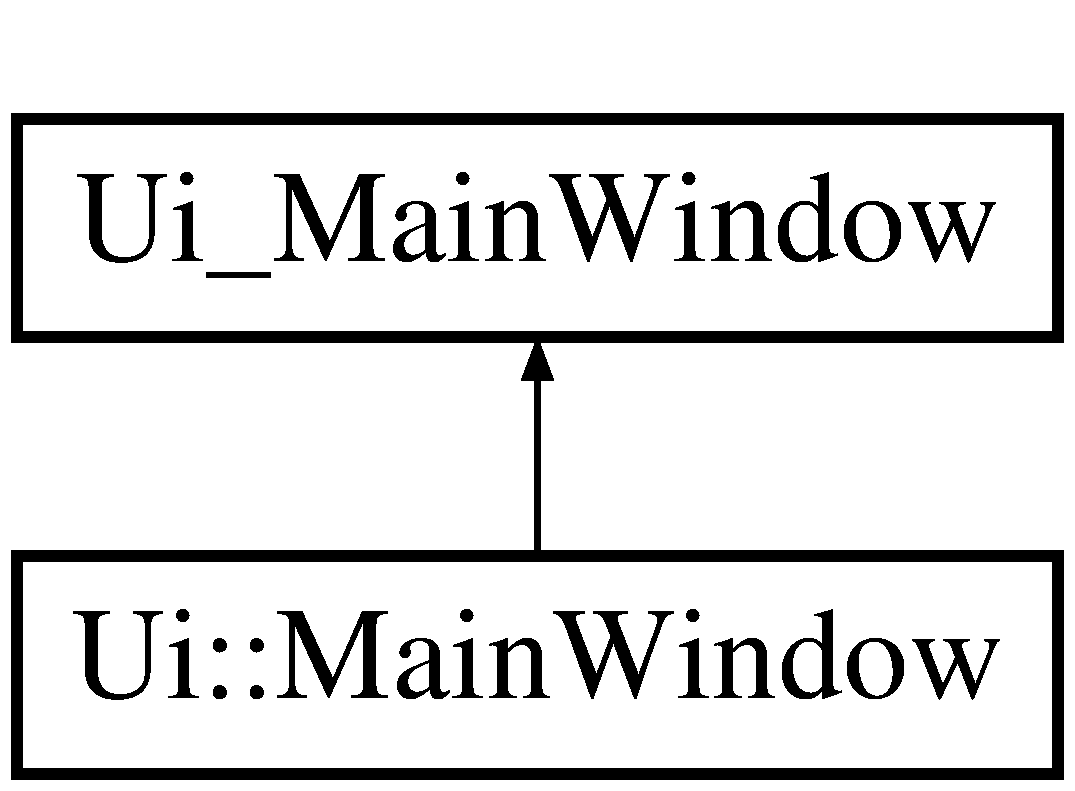
\includegraphics[height=2.000000cm]{classUi__MainWindow}
\end{center}
\end{figure}
\subsection*{\-Public \-Member \-Functions}
\begin{DoxyCompactItemize}
\item 
\hypertarget{classUi__MainWindow_acf4a0872c4c77d8f43a2ec66ed849b58}{void {\bfseries setup\-Ui} (\-Q\-Main\-Window $\ast$\hyperlink{classMainWindow}{\-Main\-Window})}\label{classUi__MainWindow_acf4a0872c4c77d8f43a2ec66ed849b58}

\item 
\hypertarget{classUi__MainWindow_a097dd160c3534a204904cb374412c618}{void {\bfseries retranslate\-Ui} (\-Q\-Main\-Window $\ast$\hyperlink{classMainWindow}{\-Main\-Window})}\label{classUi__MainWindow_a097dd160c3534a204904cb374412c618}

\end{DoxyCompactItemize}
\subsection*{\-Public \-Attributes}
\begin{DoxyCompactItemize}
\item 
\hypertarget{classUi__MainWindow_a30075506c2116c3ed4ff25e07ae75f81}{\-Q\-Widget $\ast$ {\bfseries central\-Widget}}\label{classUi__MainWindow_a30075506c2116c3ed4ff25e07ae75f81}

\item 
\hypertarget{classUi__MainWindow_a0ccfd05ec209c1a4f3a237bbb4036a9f}{\-Q\-Timer $\ast$ {\bfseries timer}}\label{classUi__MainWindow_a0ccfd05ec209c1a4f3a237bbb4036a9f}

\item 
\hypertarget{classUi__MainWindow_a00a03989019e89454f71c3ef532743db}{\-Q\-Action $\ast$ {\bfseries save\-Act}}\label{classUi__MainWindow_a00a03989019e89454f71c3ef532743db}

\item 
\hypertarget{classUi__MainWindow_aa10b3399295dbd1c7b790610aeb3f70d}{\-Q\-Action $\ast$ {\bfseries eraser\-Act}}\label{classUi__MainWindow_aa10b3399295dbd1c7b790610aeb3f70d}

\item 
\hypertarget{classUi__MainWindow_a88505412a11d7dc3040aded8f1bfda3b}{\-Q\-Action $\ast$ {\bfseries skeleton\-Act}}\label{classUi__MainWindow_a88505412a11d7dc3040aded8f1bfda3b}

\item 
\hypertarget{classUi__MainWindow_af8c83b1970227d2da8ec5c35fea2447b}{\-Q\-Action $\ast$ {\bfseries next\-Frame\-Act}}\label{classUi__MainWindow_af8c83b1970227d2da8ec5c35fea2447b}

\item 
\hypertarget{classUi__MainWindow_a47ea94c3688ac317281517ad5970eb4f}{\-Q\-Action $\ast$ {\bfseries prev\-Frame\-Act}}\label{classUi__MainWindow_a47ea94c3688ac317281517ad5970eb4f}

\item 
\hypertarget{classUi__MainWindow_a70b93096e4b1748af35d0d759d9f0dad}{\-Q\-Action $\ast$ {\bfseries rigging\-Act}}\label{classUi__MainWindow_a70b93096e4b1748af35d0d759d9f0dad}

\item 
\hypertarget{classUi__MainWindow_ab507867a4e147fac92eb0c779f01edf1}{\-Q\-Action $\ast$ {\bfseries retrieve\-Skeleton\-Act}}\label{classUi__MainWindow_ab507867a4e147fac92eb0c779f01edf1}

\item 
\hypertarget{classUi__MainWindow_ab48d681936d8c71725738b2cf8de7d52}{\-Q\-Action $\ast$ {\bfseries change\-Rig\-Points\-Act}}\label{classUi__MainWindow_ab48d681936d8c71725738b2cf8de7d52}

\item 
\hypertarget{classUi__MainWindow_a65a572f745b94dcde290bd73147a465f}{\-Q\-Action $\ast$ {\bfseries modify\-Rig\-Act}}\label{classUi__MainWindow_a65a572f745b94dcde290bd73147a465f}

\item 
\hypertarget{classUi__MainWindow_a80ba56842e4803e3ac2ddb492ffa024b}{\-Q\-Action $\ast$ {\bfseries update\-Shadow\-Act}}\label{classUi__MainWindow_a80ba56842e4803e3ac2ddb492ffa024b}

\item 
\hypertarget{classUi__MainWindow_accac35ef0f2de62e207a9e6867984a84}{\-Q\-Action $\ast$ {\bfseries redraw\-Skeleton\-Act}}\label{classUi__MainWindow_accac35ef0f2de62e207a9e6867984a84}

\item 
\hypertarget{classUi__MainWindow_a686f2529aa9bae8cc1540adfeb991cfb}{\-Q\-Spin\-Box $\ast$ {\bfseries spinner}}\label{classUi__MainWindow_a686f2529aa9bae8cc1540adfeb991cfb}

\item 
\hypertarget{classUi__MainWindow_a1ac28e051d155da0fe23d8553df17bfd}{\-Q\-Slider $\ast$ {\bfseries slider}}\label{classUi__MainWindow_a1ac28e051d155da0fe23d8553df17bfd}

\item 
\hypertarget{classUi__MainWindow_a03ce63974cc69b067c91bbf285cceca8}{\-Q\-H\-Box\-Layout $\ast$ {\bfseries horizontal\-Layout\-\_\-3}}\label{classUi__MainWindow_a03ce63974cc69b067c91bbf285cceca8}

\item 
\hypertarget{classUi__MainWindow_a80867018070156432923d0266cc9fe25}{\-Q\-H\-Box\-Layout $\ast$ {\bfseries horizontal\-Layout\-\_\-2}}\label{classUi__MainWindow_a80867018070156432923d0266cc9fe25}

\item 
\hypertarget{classUi__MainWindow_a0c01bad60d9f422a1258e710635a2f65}{\-Q\-V\-Box\-Layout $\ast$ {\bfseries vertical\-Layout\-\_\-2}}\label{classUi__MainWindow_a0c01bad60d9f422a1258e710635a2f65}

\item 
\hypertarget{classUi__MainWindow_a0004ce950eac6d07f19fca1fda0d65fe}{\hyperlink{classScribbleArea}{\-Scribble\-Area} $\ast$ {\bfseries scribble\-Area}}\label{classUi__MainWindow_a0004ce950eac6d07f19fca1fda0d65fe}

\item 
\hypertarget{classUi__MainWindow_a955cbbea2ef1a9929c3daf38b0a6dcd5}{\-Q\-Text\-Edit $\ast$ {\bfseries text\-Edit}}\label{classUi__MainWindow_a955cbbea2ef1a9929c3daf38b0a6dcd5}

\item 
\hypertarget{classUi__MainWindow_a38b8a4b887f3b58e2a49e7905ae6f1f0}{\-Q\-V\-Box\-Layout $\ast$ {\bfseries vertical\-Layout\-\_\-3}}\label{classUi__MainWindow_a38b8a4b887f3b58e2a49e7905ae6f1f0}

\item 
\hypertarget{classUi__MainWindow_a6f40fc110b15410c00837a446d57bdbe}{\-Q\-V\-Box\-Layout $\ast$ {\bfseries vertical\-Layout\-\_\-4}}\label{classUi__MainWindow_a6f40fc110b15410c00837a446d57bdbe}

\item 
\hypertarget{classUi__MainWindow_aecd96a04789fcfec3f98d80390ad8184}{\-Q\-V\-Box\-Layout $\ast$ {\bfseries vertical\-Layout}}\label{classUi__MainWindow_aecd96a04789fcfec3f98d80390ad8184}

\item 
\hypertarget{classUi__MainWindow_a975db6b4a3887d5ba1b357208b9b2593}{\-Q\-Push\-Button $\ast$ {\bfseries \-Shadow}}\label{classUi__MainWindow_a975db6b4a3887d5ba1b357208b9b2593}

\item 
\hypertarget{classUi__MainWindow_a5810c012ea165398037b446bf7d3ea68}{\-Q\-Push\-Button $\ast$ {\bfseries \-Skeleton}}\label{classUi__MainWindow_a5810c012ea165398037b446bf7d3ea68}

\item 
\hypertarget{classUi__MainWindow_a53080a27b056365ab1d4c7cd0365f236}{\-Q\-Push\-Button $\ast$ {\bfseries \-Sketch}}\label{classUi__MainWindow_a53080a27b056365ab1d4c7cd0365f236}

\item 
\hypertarget{classUi__MainWindow_a0a309e2ddb7a52e876104e6da6d36a3e}{\-Q\-Push\-Button $\ast$ {\bfseries \-Normal}}\label{classUi__MainWindow_a0a309e2ddb7a52e876104e6da6d36a3e}

\item 
\hypertarget{classUi__MainWindow_ae541f12c68bc3d241f2651ca1c830918}{\-Q\-Push\-Button $\ast$ {\bfseries \-Erase}}\label{classUi__MainWindow_ae541f12c68bc3d241f2651ca1c830918}

\item 
\hypertarget{classUi__MainWindow_a2cde0ec9b2a1b129d77c8732df6792b8}{\-Q\-Push\-Button $\ast$ {\bfseries \-Play}}\label{classUi__MainWindow_a2cde0ec9b2a1b129d77c8732df6792b8}

\item 
\hypertarget{classUi__MainWindow_ade1786a3d33551c3af353c2bc84e8517}{\-Q\-Push\-Button $\ast$ {\bfseries \-Stop}}\label{classUi__MainWindow_ade1786a3d33551c3af353c2bc84e8517}

\item 
\hypertarget{classUi__MainWindow_a2be1c24ec9adfca18e1dcc951931457f}{\-Q\-Menu\-Bar $\ast$ {\bfseries menu\-Bar}}\label{classUi__MainWindow_a2be1c24ec9adfca18e1dcc951931457f}

\item 
\hypertarget{classUi__MainWindow_a5172877001c8c7b4e0f6de50421867d1}{\-Q\-Tool\-Bar $\ast$ {\bfseries main\-Tool\-Bar}}\label{classUi__MainWindow_a5172877001c8c7b4e0f6de50421867d1}

\item 
\hypertarget{classUi__MainWindow_a50fa481337604bcc8bf68de18ab16ecd}{\-Q\-Status\-Bar $\ast$ {\bfseries status\-Bar}}\label{classUi__MainWindow_a50fa481337604bcc8bf68de18ab16ecd}

\item 
\hypertarget{classUi__MainWindow_a9dc4dba26b83e0c94aa566e1c564420b}{\-Q\-Label $\ast$ {\bfseries label\-\_\-10}}\label{classUi__MainWindow_a9dc4dba26b83e0c94aa566e1c564420b}

\end{DoxyCompactItemize}


\-The documentation for this class was generated from the following file\-:\begin{DoxyCompactItemize}
\item 
/home/priyanka/\-Dataset25/src/\-G\-U\-I/ui\-\_\-mainwindow.\-h\end{DoxyCompactItemize}

\hypertarget{classutil_1_1math_1_1vec2}{\section{util\-:\-:math\-:\-:vec2 \-Class \-Reference}
\label{classutil_1_1math_1_1vec2}\index{util\-::math\-::vec2@{util\-::math\-::vec2}}
}


\-This is a general 2\-D vector class.  




{\ttfamily \#include $<$matvec.\-hpp$>$}

\subsection*{\-Public \-Member \-Functions}
\begin{DoxyCompactItemize}
\item 
\hypertarget{classutil_1_1math_1_1vec2_af368a5df5d0de984e45879db971b1d04}{\hyperlink{classutil_1_1math_1_1vec2_af368a5df5d0de984e45879db971b1d04}{vec2} (const \hyperlink{classutil_1_1math_1_1vec3}{vec3} \&v)}\label{classutil_1_1math_1_1vec2_af368a5df5d0de984e45879db971b1d04}

\begin{DoxyCompactList}\small\item\em \-Downcasting from a 3\-D vector to 2\-D. \end{DoxyCompactList}\item 
\hypertarget{classutil_1_1math_1_1vec2_a6f53edc9e89672d0164d8428a023d772}{\hyperlink{classutil_1_1math_1_1vec2_a6f53edc9e89672d0164d8428a023d772}{vec2} (const \hyperlink{classutil_1_1math_1_1vec3}{vec3} \&v, int drop\-Axis)}\label{classutil_1_1math_1_1vec2_a6f53edc9e89672d0164d8428a023d772}

\begin{DoxyCompactList}\small\item\em \-Downcasting from a 3\-D vector to 2\-D, dropping the `drop\-Axis' component. \end{DoxyCompactList}\item 
\hypertarget{classutil_1_1math_1_1vec2_a2b4006cca4db9c4353d2bda6a6d18f44}{\hyperlink{classutil_1_1math_1_1vec2_a2b4006cca4db9c4353d2bda6a6d18f44}{$\sim$vec2} ()}\label{classutil_1_1math_1_1vec2_a2b4006cca4db9c4353d2bda6a6d18f44}

\begin{DoxyCompactList}\small\item\em \-Destructor. \end{DoxyCompactList}\item 
\hypertarget{classutil_1_1math_1_1vec2_a2ab5b563ceb76bc4d89349483ed50266}{double \& \hyperlink{classutil_1_1math_1_1vec2_a2ab5b563ceb76bc4d89349483ed50266}{operator\mbox{[}$\,$\mbox{]}} (int index)}\label{classutil_1_1math_1_1vec2_a2ab5b563ceb76bc4d89349483ed50266}

\begin{DoxyCompactList}\small\item\em \-Overloaded indexing operator. \end{DoxyCompactList}\item 
\hypertarget{classutil_1_1math_1_1vec2_ac7b3726914c70788f22e7c2719d256a0}{double \hyperlink{classutil_1_1math_1_1vec2_ac7b3726914c70788f22e7c2719d256a0}{operator\mbox{[}$\,$\mbox{]}} (int index) const }\label{classutil_1_1math_1_1vec2_ac7b3726914c70788f22e7c2719d256a0}

\begin{DoxyCompactList}\small\item\em \-Overloaded indexing operator. \end{DoxyCompactList}\item 
\hypertarget{classutil_1_1math_1_1vec2_a4a9e60b6a39005ae2d0d5737c6b42e56}{double \hyperlink{classutil_1_1math_1_1vec2_a4a9e60b6a39005ae2d0d5737c6b42e56}{length} (void) const }\label{classutil_1_1math_1_1vec2_a4a9e60b6a39005ae2d0d5737c6b42e56}

\begin{DoxyCompactList}\small\item\em \-Returns length of the vector. \end{DoxyCompactList}\item 
\hypertarget{classutil_1_1math_1_1vec2_aa2fe7d50439069bab5d2000aee53b478}{double \hyperlink{classutil_1_1math_1_1vec2_aa2fe7d50439069bab5d2000aee53b478}{length2} (void) const }\label{classutil_1_1math_1_1vec2_aa2fe7d50439069bab5d2000aee53b478}

\begin{DoxyCompactList}\small\item\em \-Returns squared length of the vector. \end{DoxyCompactList}\item 
\hypertarget{classutil_1_1math_1_1vec2_aecc0661c87eefee1c9cded894085f570}{\hyperlink{classutil_1_1math_1_1vec2}{vec2} \& \hyperlink{classutil_1_1math_1_1vec2_aecc0661c87eefee1c9cded894085f570}{normalize} (void)}\label{classutil_1_1math_1_1vec2_aecc0661c87eefee1c9cded894085f570}

\begin{DoxyCompactList}\small\item\em \-Normalizes the vector. \end{DoxyCompactList}\item 
\hypertarget{classutil_1_1math_1_1vec2_abc93e936c64163bf51dc624eb4e83d18}{\hyperlink{classutil_1_1math_1_1vec2}{vec2} \& \hyperlink{classutil_1_1math_1_1vec2_abc93e936c64163bf51dc624eb4e83d18}{map} (double($\ast$fn)(double))}\label{classutil_1_1math_1_1vec2_abc93e936c64163bf51dc624eb4e83d18}

\begin{DoxyCompactList}\small\item\em \-Maps the function to every component of the vector. \end{DoxyCompactList}\item 
\hypertarget{classutil_1_1math_1_1vec2_ae6a974371b4c2eaf4eb230207ad9d866}{void \hyperlink{classutil_1_1math_1_1vec2_ae6a974371b4c2eaf4eb230207ad9d866}{set} (double x, double y)}\label{classutil_1_1math_1_1vec2_ae6a974371b4c2eaf4eb230207ad9d866}

\begin{DoxyCompactList}\small\item\em \-Sets the value of the vector. \end{DoxyCompactList}\item 
\hypertarget{classutil_1_1math_1_1vec2_a82af13736db6f94614025a32facf1f9c}{void \hyperlink{classutil_1_1math_1_1vec2_a82af13736db6f94614025a32facf1f9c}{print} (\-F\-I\-L\-E $\ast$file, std\-::string name)}\label{classutil_1_1math_1_1vec2_a82af13736db6f94614025a32facf1f9c}

\begin{DoxyCompactList}\small\item\em \-Prints the vector into a file. \end{DoxyCompactList}\end{DoxyCompactItemize}
{\bf }\par
\begin{DoxyCompactItemize}
\item 
\hypertarget{classutil_1_1math_1_1vec2_ab4e9fb7dc8c8f3b822617657843d970a}{\hyperlink{classutil_1_1math_1_1vec2_ab4e9fb7dc8c8f3b822617657843d970a}{vec2} ()}\label{classutil_1_1math_1_1vec2_ab4e9fb7dc8c8f3b822617657843d970a}

\begin{DoxyCompactList}\small\item\em \-Constructor. \end{DoxyCompactList}\item 
\hypertarget{classutil_1_1math_1_1vec2_a0281180cc2a94899566d87edbb45e214}{{\bfseries vec2} (const double x, const double y)}\label{classutil_1_1math_1_1vec2_a0281180cc2a94899566d87edbb45e214}

\item 
\hypertarget{classutil_1_1math_1_1vec2_aa501b7322c72c0155bdd5236bd397b3e}{{\bfseries vec2} (const double d)}\label{classutil_1_1math_1_1vec2_aa501b7322c72c0155bdd5236bd397b3e}

\item 
\hypertarget{classutil_1_1math_1_1vec2_a67759c5e3719848e3e5aaf8e11103a0a}{{\bfseries vec2} (const double v\mbox{[}2\mbox{]})}\label{classutil_1_1math_1_1vec2_a67759c5e3719848e3e5aaf8e11103a0a}

\item 
\hypertarget{classutil_1_1math_1_1vec2_a2e4c97f36d5362ff6c31160c06d162c6}{{\bfseries vec2} (const \hyperlink{classutil_1_1math_1_1vec2}{vec2} \&v)}\label{classutil_1_1math_1_1vec2_a2e4c97f36d5362ff6c31160c06d162c6}

\end{DoxyCompactItemize}

{\bf }\par
\begin{DoxyCompactItemize}
\item 
\hypertarget{classutil_1_1math_1_1vec2_a1b426b87094d796cfbee3d7b9fbea9ca}{\hyperlink{classutil_1_1math_1_1vec2}{vec2} \& \hyperlink{classutil_1_1math_1_1vec2_a1b426b87094d796cfbee3d7b9fbea9ca}{operator=} (const \hyperlink{classutil_1_1math_1_1vec2}{vec2} \&v)}\label{classutil_1_1math_1_1vec2_a1b426b87094d796cfbee3d7b9fbea9ca}

\begin{DoxyCompactList}\small\item\em \-Overloaded assignment operators. \end{DoxyCompactList}\item 
\hypertarget{classutil_1_1math_1_1vec2_aa40c76bb6d5126163e773422c5e6e83d}{\hyperlink{classutil_1_1math_1_1vec2}{vec2} \& {\bfseries operator+=} (const \hyperlink{classutil_1_1math_1_1vec2}{vec2} \&v)}\label{classutil_1_1math_1_1vec2_aa40c76bb6d5126163e773422c5e6e83d}

\item 
\hypertarget{classutil_1_1math_1_1vec2_a0b07b5a1347d0da988c92aa766123f7a}{\hyperlink{classutil_1_1math_1_1vec2}{vec2} \& {\bfseries operator-\/=} (const \hyperlink{classutil_1_1math_1_1vec2}{vec2} \&v)}\label{classutil_1_1math_1_1vec2_a0b07b5a1347d0da988c92aa766123f7a}

\item 
\hypertarget{classutil_1_1math_1_1vec2_a0b77d5a948fb88a324b0b3c78788b2fe}{\hyperlink{classutil_1_1math_1_1vec2}{vec2} \& {\bfseries operator$\ast$=} (const double d)}\label{classutil_1_1math_1_1vec2_a0b77d5a948fb88a324b0b3c78788b2fe}

\item 
\hypertarget{classutil_1_1math_1_1vec2_aea5c1792da9a12650124a8152dd3acc5}{\hyperlink{classutil_1_1math_1_1vec2}{vec2} \& {\bfseries operator/=} (const double d)}\label{classutil_1_1math_1_1vec2_aea5c1792da9a12650124a8152dd3acc5}

\end{DoxyCompactItemize}

\subsection*{\-Protected \-Attributes}
\begin{DoxyCompactItemize}
\item 
\hypertarget{classutil_1_1math_1_1vec2_a99cfcabc1e89091eb63d17c565a334d7}{double \hyperlink{classutil_1_1math_1_1vec2_a99cfcabc1e89091eb63d17c565a334d7}{data} \mbox{[}2\mbox{]}}\label{classutil_1_1math_1_1vec2_a99cfcabc1e89091eb63d17c565a334d7}

\begin{DoxyCompactList}\small\item\em \-The two data components of the vector. \end{DoxyCompactList}\end{DoxyCompactItemize}
\subsection*{\-Friends}
\begin{DoxyCompactItemize}
\item 
\hypertarget{classutil_1_1math_1_1vec2_aa849243c6cd858bbcd88237a8ad16cad}{class \hyperlink{classutil_1_1math_1_1vec2_aa849243c6cd858bbcd88237a8ad16cad}{vec3}}\label{classutil_1_1math_1_1vec2_aa849243c6cd858bbcd88237a8ad16cad}

\begin{DoxyCompactList}\small\item\em \-Friend class. \end{DoxyCompactList}\item 
\hypertarget{classutil_1_1math_1_1vec2_a4a372204e9d4fbce7b21ba855dc5e567}{\hyperlink{classutil_1_1math_1_1vec2}{vec2} \hyperlink{classutil_1_1math_1_1vec2_a4a372204e9d4fbce7b21ba855dc5e567}{operator-\/} (const \hyperlink{classutil_1_1math_1_1vec2}{vec2} \&v)}\label{classutil_1_1math_1_1vec2_a4a372204e9d4fbce7b21ba855dc5e567}

\begin{DoxyCompactList}\small\item\em \-Overloaded unary negation. \end{DoxyCompactList}\item 
\hypertarget{classutil_1_1math_1_1vec2_a16e78f0abc6889e956835d00606a4fbd}{\hyperlink{classutil_1_1math_1_1vec2}{vec2} \hyperlink{classutil_1_1math_1_1vec2_a16e78f0abc6889e956835d00606a4fbd}{operator+} (const \hyperlink{classutil_1_1math_1_1vec2}{vec2} \&v1, const \hyperlink{classutil_1_1math_1_1vec2}{vec2} \&v2)}\label{classutil_1_1math_1_1vec2_a16e78f0abc6889e956835d00606a4fbd}

\begin{DoxyCompactList}\small\item\em \-Overloaded addition. \end{DoxyCompactList}\item 
\hypertarget{classutil_1_1math_1_1vec2_a5b94d4dd9df52ab156e5a65562f3e088}{\hyperlink{classutil_1_1math_1_1vec2}{vec2} \hyperlink{classutil_1_1math_1_1vec2_a5b94d4dd9df52ab156e5a65562f3e088}{operator-\/} (const \hyperlink{classutil_1_1math_1_1vec2}{vec2} \&v1, const \hyperlink{classutil_1_1math_1_1vec2}{vec2} \&v2)}\label{classutil_1_1math_1_1vec2_a5b94d4dd9df52ab156e5a65562f3e088}

\begin{DoxyCompactList}\small\item\em \-Overloaded subtraction. \end{DoxyCompactList}\item 
\hypertarget{classutil_1_1math_1_1vec2_a6aa3cf219cbdd3248b18830402caef79}{\hyperlink{classutil_1_1math_1_1vec2}{vec2} \hyperlink{classutil_1_1math_1_1vec2_a6aa3cf219cbdd3248b18830402caef79}{operator$\ast$} (const \hyperlink{classutil_1_1math_1_1vec2}{vec2} \&v, const double d)}\label{classutil_1_1math_1_1vec2_a6aa3cf219cbdd3248b18830402caef79}

\begin{DoxyCompactList}\small\item\em \-Overloaded multiplication (vector \& constant) \end{DoxyCompactList}\item 
\hypertarget{classutil_1_1math_1_1vec2_a6d2946077a1f064e83e84abbc45d4729}{\hyperlink{classutil_1_1math_1_1vec2}{vec2} \hyperlink{classutil_1_1math_1_1vec2_a6d2946077a1f064e83e84abbc45d4729}{operator$\ast$} (const double d, const \hyperlink{classutil_1_1math_1_1vec2}{vec2} \&v)}\label{classutil_1_1math_1_1vec2_a6d2946077a1f064e83e84abbc45d4729}

\begin{DoxyCompactList}\small\item\em \-Overloaded multiplication (constant \& vector) \end{DoxyCompactList}\item 
\hypertarget{classutil_1_1math_1_1vec2_afe24dc4fe91537d7af200c5b3780edd9}{double \hyperlink{classutil_1_1math_1_1vec2_afe24dc4fe91537d7af200c5b3780edd9}{operator$\ast$} (const \hyperlink{classutil_1_1math_1_1vec2}{vec2} \&v1, const \hyperlink{classutil_1_1math_1_1vec2}{vec2} \&v2)}\label{classutil_1_1math_1_1vec2_afe24dc4fe91537d7af200c5b3780edd9}

\begin{DoxyCompactList}\small\item\em \-Overloaded multiplication (dot product) \end{DoxyCompactList}\item 
\hypertarget{classutil_1_1math_1_1vec2_acaac30f3de430cef9803df6f77f2184e}{\hyperlink{classutil_1_1math_1_1vec2}{vec2} \hyperlink{classutil_1_1math_1_1vec2_acaac30f3de430cef9803df6f77f2184e}{operator/} (const \hyperlink{classutil_1_1math_1_1vec2}{vec2} \&v, const double d)}\label{classutil_1_1math_1_1vec2_acaac30f3de430cef9803df6f77f2184e}

\begin{DoxyCompactList}\small\item\em \-Oveloaded division (vector \& constant) \end{DoxyCompactList}\item 
\hypertarget{classutil_1_1math_1_1vec2_a281f90be035f93a30c91b37ec06b798f}{\hyperlink{classutil_1_1math_1_1vec3}{vec3} \hyperlink{classutil_1_1math_1_1vec2_a281f90be035f93a30c91b37ec06b798f}{operator$^\wedge$} (const \hyperlink{classutil_1_1math_1_1vec2}{vec2} \&v1, const \hyperlink{classutil_1_1math_1_1vec2}{vec2} \&v2)}\label{classutil_1_1math_1_1vec2_a281f90be035f93a30c91b37ec06b798f}

\begin{DoxyCompactList}\small\item\em \-Vector cross product. \end{DoxyCompactList}\item 
\hypertarget{classutil_1_1math_1_1vec2_a0f20d5eff5576157b355c3e4256dafc7}{bool \hyperlink{classutil_1_1math_1_1vec2_a0f20d5eff5576157b355c3e4256dafc7}{operator==} (const \hyperlink{classutil_1_1math_1_1vec2}{vec2} \&v1, const \hyperlink{classutil_1_1math_1_1vec2}{vec2} \&v2)}\label{classutil_1_1math_1_1vec2_a0f20d5eff5576157b355c3e4256dafc7}

\begin{DoxyCompactList}\small\item\em \-Vector equality. \end{DoxyCompactList}\item 
\hypertarget{classutil_1_1math_1_1vec2_ab8bee146ca4567b7bf5deb7276b54d08}{bool \hyperlink{classutil_1_1math_1_1vec2_ab8bee146ca4567b7bf5deb7276b54d08}{operator!=} (const \hyperlink{classutil_1_1math_1_1vec2}{vec2} \&v1, const \hyperlink{classutil_1_1math_1_1vec2}{vec2} \&v2)}\label{classutil_1_1math_1_1vec2_ab8bee146ca4567b7bf5deb7276b54d08}

\begin{DoxyCompactList}\small\item\em \-Vector inequality. \end{DoxyCompactList}\item 
\hypertarget{classutil_1_1math_1_1vec2_adea6024eac5b48729c1e9149c98d0158}{void \hyperlink{classutil_1_1math_1_1vec2_adea6024eac5b48729c1e9149c98d0158}{swap} (\hyperlink{classutil_1_1math_1_1vec2}{vec2} \&v1, \hyperlink{classutil_1_1math_1_1vec2}{vec2} \&v2)}\label{classutil_1_1math_1_1vec2_adea6024eac5b48729c1e9149c98d0158}

\begin{DoxyCompactList}\small\item\em \-Swap vectors v1 and v2. \end{DoxyCompactList}\item 
\hypertarget{classutil_1_1math_1_1vec2_a46ee1742ead8ea22dcb111bfb9fa40ab}{\hyperlink{classutil_1_1math_1_1vec2}{vec2} \hyperlink{classutil_1_1math_1_1vec2_a46ee1742ead8ea22dcb111bfb9fa40ab}{min} (const \hyperlink{classutil_1_1math_1_1vec2}{vec2} \&v1, const \hyperlink{classutil_1_1math_1_1vec2}{vec2} \&v2)}\label{classutil_1_1math_1_1vec2_a46ee1742ead8ea22dcb111bfb9fa40ab}

\begin{DoxyCompactList}\small\item\em \-Minimum of vectors v1 \& v2. \end{DoxyCompactList}\item 
\hypertarget{classutil_1_1math_1_1vec2_aa059546101199b29146ae8283cc0ae9a}{\hyperlink{classutil_1_1math_1_1vec2}{vec2} \hyperlink{classutil_1_1math_1_1vec2_aa059546101199b29146ae8283cc0ae9a}{max} (const \hyperlink{classutil_1_1math_1_1vec2}{vec2} \&v1, const \hyperlink{classutil_1_1math_1_1vec2}{vec2} \&v2)}\label{classutil_1_1math_1_1vec2_aa059546101199b29146ae8283cc0ae9a}

\begin{DoxyCompactList}\small\item\em \-Maximum of vectors v1 \& v2. \end{DoxyCompactList}\item 
\hypertarget{classutil_1_1math_1_1vec2_a9a7afb1a742384c7a7801658736f8264}{\hyperlink{classutil_1_1math_1_1vec2}{vec2} \hyperlink{classutil_1_1math_1_1vec2_a9a7afb1a742384c7a7801658736f8264}{prod} (const \hyperlink{classutil_1_1math_1_1vec2}{vec2} \&v1, const \hyperlink{classutil_1_1math_1_1vec2}{vec2} \&v2)}\label{classutil_1_1math_1_1vec2_a9a7afb1a742384c7a7801658736f8264}

\begin{DoxyCompactList}\small\item\em \-Term by term product. \end{DoxyCompactList}\end{DoxyCompactItemize}


\subsection{\-Detailed \-Description}
\-This is a general 2\-D vector class. 

\-The documentation for this class was generated from the following files\-:\begin{DoxyCompactItemize}
\item 
/home/priyanka/\-Dataset25/src/\-G\-U\-I/\hyperlink{matvec_8hpp}{matvec.\-hpp}\item 
/home/priyanka/\-Dataset25/src/\-G\-U\-I/matvec.\-cpp\end{DoxyCompactItemize}

\hypertarget{classutil_1_1math_1_1vec3}{\section{util\-:\-:math\-:\-:vec3 \-Class \-Reference}
\label{classutil_1_1math_1_1vec3}\index{util\-::math\-::vec3@{util\-::math\-::vec3}}
}


\-This is a general 3\-D vector class.  




{\ttfamily \#include $<$matvec.\-hpp$>$}

\subsection*{\-Public \-Member \-Functions}
\begin{DoxyCompactItemize}
\item 
\hypertarget{classutil_1_1math_1_1vec3_aa76ecb2e2e4169d0719e70d928cbb9f5}{\hyperlink{classutil_1_1math_1_1vec3_aa76ecb2e2e4169d0719e70d928cbb9f5}{vec3} (const \hyperlink{classutil_1_1math_1_1vec4}{vec4} \&v)}\label{classutil_1_1math_1_1vec3_aa76ecb2e2e4169d0719e70d928cbb9f5}

\begin{DoxyCompactList}\small\item\em \-Downcasting from a 4\-D vector to 3\-D. \end{DoxyCompactList}\item 
\hypertarget{classutil_1_1math_1_1vec3_ac1432a40730a7919dddecbb5042e4cee}{\hyperlink{classutil_1_1math_1_1vec3_ac1432a40730a7919dddecbb5042e4cee}{vec3} (const \hyperlink{classutil_1_1math_1_1vec4}{vec4} \&v, int drop\-Axis)}\label{classutil_1_1math_1_1vec3_ac1432a40730a7919dddecbb5042e4cee}

\begin{DoxyCompactList}\small\item\em \-Downcasting from a 4\-D vector to 3\-D, dropping the `drop\-Axis' component. \end{DoxyCompactList}\item 
\hypertarget{classutil_1_1math_1_1vec3_af8045fb15a617d99b9ac76c6af04f6c8}{\hyperlink{classutil_1_1math_1_1vec3_af8045fb15a617d99b9ac76c6af04f6c8}{$\sim$vec3} ()}\label{classutil_1_1math_1_1vec3_af8045fb15a617d99b9ac76c6af04f6c8}

\begin{DoxyCompactList}\small\item\em \-Destructor. \end{DoxyCompactList}\item 
\hypertarget{classutil_1_1math_1_1vec3_aaf6301c10fd53827c56a481703202d1e}{double \& \hyperlink{classutil_1_1math_1_1vec3_aaf6301c10fd53827c56a481703202d1e}{operator\mbox{[}$\,$\mbox{]}} (int index)}\label{classutil_1_1math_1_1vec3_aaf6301c10fd53827c56a481703202d1e}

\begin{DoxyCompactList}\small\item\em \-Overloaded indexing operator. \end{DoxyCompactList}\item 
\hypertarget{classutil_1_1math_1_1vec3_a902087b3ff44eb916fd13941354c66ed}{double \hyperlink{classutil_1_1math_1_1vec3_a902087b3ff44eb916fd13941354c66ed}{operator\mbox{[}$\,$\mbox{]}} (int index) const }\label{classutil_1_1math_1_1vec3_a902087b3ff44eb916fd13941354c66ed}

\begin{DoxyCompactList}\small\item\em \-Overloaded indexing operator. \end{DoxyCompactList}\item 
\hypertarget{classutil_1_1math_1_1vec3_a15ddc56b3ad8fb6fcd0063da0558f7c9}{double \hyperlink{classutil_1_1math_1_1vec3_a15ddc56b3ad8fb6fcd0063da0558f7c9}{length} (void) const }\label{classutil_1_1math_1_1vec3_a15ddc56b3ad8fb6fcd0063da0558f7c9}

\begin{DoxyCompactList}\small\item\em \-Returns length of the vector. \end{DoxyCompactList}\item 
\hypertarget{classutil_1_1math_1_1vec3_ab1c1a11be9fdb31c4e85091d9283fc9c}{double \hyperlink{classutil_1_1math_1_1vec3_ab1c1a11be9fdb31c4e85091d9283fc9c}{length2} (void) const }\label{classutil_1_1math_1_1vec3_ab1c1a11be9fdb31c4e85091d9283fc9c}

\begin{DoxyCompactList}\small\item\em \-Returns squared length of the vector. \end{DoxyCompactList}\item 
\hypertarget{classutil_1_1math_1_1vec3_a659cf322957535bf345b673ecc6c672d}{\hyperlink{classutil_1_1math_1_1vec3}{vec3} \& \hyperlink{classutil_1_1math_1_1vec3_a659cf322957535bf345b673ecc6c672d}{normalize} (void)}\label{classutil_1_1math_1_1vec3_a659cf322957535bf345b673ecc6c672d}

\begin{DoxyCompactList}\small\item\em \-Normalizes the vector. \end{DoxyCompactList}\item 
\hypertarget{classutil_1_1math_1_1vec3_a302ce4196f7b18279b47c063d3db3887}{\hyperlink{classutil_1_1math_1_1vec3}{vec3} \& \hyperlink{classutil_1_1math_1_1vec3_a302ce4196f7b18279b47c063d3db3887}{homogenize} (void)}\label{classutil_1_1math_1_1vec3_a302ce4196f7b18279b47c063d3db3887}

\begin{DoxyCompactList}\small\item\em \-Homogenizes the vector. \end{DoxyCompactList}\item 
\hypertarget{classutil_1_1math_1_1vec3_a00f991fca6808eeebb252ce167f78a8c}{\hyperlink{classutil_1_1math_1_1vec3}{vec3} \& \hyperlink{classutil_1_1math_1_1vec3_a00f991fca6808eeebb252ce167f78a8c}{map} (double($\ast$fn)(double))}\label{classutil_1_1math_1_1vec3_a00f991fca6808eeebb252ce167f78a8c}

\begin{DoxyCompactList}\small\item\em \-Maps the function to every component of the vector. \end{DoxyCompactList}\item 
\hypertarget{classutil_1_1math_1_1vec3_ac564460ee54987dc39cf577285701816}{void \hyperlink{classutil_1_1math_1_1vec3_ac564460ee54987dc39cf577285701816}{set} (double x, double y, double z)}\label{classutil_1_1math_1_1vec3_ac564460ee54987dc39cf577285701816}

\begin{DoxyCompactList}\small\item\em \-Sets the value of the vector. \end{DoxyCompactList}\item 
\hypertarget{classutil_1_1math_1_1vec3_afd20d73037ce507437fe2f08ba0a3d07}{void \hyperlink{classutil_1_1math_1_1vec3_afd20d73037ce507437fe2f08ba0a3d07}{print} (\-F\-I\-L\-E $\ast$file, std\-::string name)}\label{classutil_1_1math_1_1vec3_afd20d73037ce507437fe2f08ba0a3d07}

\begin{DoxyCompactList}\small\item\em \-Print the vector to a file. \end{DoxyCompactList}\end{DoxyCompactItemize}
{\bf }\par
\begin{DoxyCompactItemize}
\item 
\hypertarget{classutil_1_1math_1_1vec3_a947428533e7d4d35e51871e7d2b8b51a}{\hyperlink{classutil_1_1math_1_1vec3_a947428533e7d4d35e51871e7d2b8b51a}{vec3} ()}\label{classutil_1_1math_1_1vec3_a947428533e7d4d35e51871e7d2b8b51a}

\begin{DoxyCompactList}\small\item\em \-Constructor. \end{DoxyCompactList}\item 
\hypertarget{classutil_1_1math_1_1vec3_a58447a9fc69cc0ff2fba1aecf6b7c05f}{{\bfseries vec3} (const double x, const double y, const double z)}\label{classutil_1_1math_1_1vec3_a58447a9fc69cc0ff2fba1aecf6b7c05f}

\item 
\hypertarget{classutil_1_1math_1_1vec3_aa7589bf7977bbdb34cd017cbd54f618a}{{\bfseries vec3} (const double d)}\label{classutil_1_1math_1_1vec3_aa7589bf7977bbdb34cd017cbd54f618a}

\item 
\hypertarget{classutil_1_1math_1_1vec3_a47460f0b21a74011595c992320c2fc0b}{{\bfseries vec3} (const double v\mbox{[}3\mbox{]})}\label{classutil_1_1math_1_1vec3_a47460f0b21a74011595c992320c2fc0b}

\item 
\hypertarget{classutil_1_1math_1_1vec3_a9a63e151f3627c80c68fc3c254c78a34}{{\bfseries vec3} (const \hyperlink{classutil_1_1math_1_1vec3}{vec3} \&v)}\label{classutil_1_1math_1_1vec3_a9a63e151f3627c80c68fc3c254c78a34}

\end{DoxyCompactItemize}

{\bf }\par
\begin{DoxyCompactItemize}
\item 
\hypertarget{classutil_1_1math_1_1vec3_a8a3836e36c8012d2fdde753644574508}{\hyperlink{classutil_1_1math_1_1vec3_a8a3836e36c8012d2fdde753644574508}{vec3} (const \hyperlink{classutil_1_1math_1_1vec2}{vec2} \&v)}\label{classutil_1_1math_1_1vec3_a8a3836e36c8012d2fdde753644574508}

\begin{DoxyCompactList}\small\item\em \-Casting from a 2\-D vector to 3\-D. \end{DoxyCompactList}\item 
\hypertarget{classutil_1_1math_1_1vec3_a4a4505f01fe537b644f7e1f8679e5703}{{\bfseries vec3} (const \hyperlink{classutil_1_1math_1_1vec2}{vec2} \&v, double d)}\label{classutil_1_1math_1_1vec3_a4a4505f01fe537b644f7e1f8679e5703}

\end{DoxyCompactItemize}

{\bf }\par
\begin{DoxyCompactItemize}
\item 
\hypertarget{classutil_1_1math_1_1vec3_a69dc97259ead3f6adfe400a8c9c97732}{\hyperlink{classutil_1_1math_1_1vec3}{vec3} \& \hyperlink{classutil_1_1math_1_1vec3_a69dc97259ead3f6adfe400a8c9c97732}{operator=} (const \hyperlink{classutil_1_1math_1_1vec3}{vec3} \&v)}\label{classutil_1_1math_1_1vec3_a69dc97259ead3f6adfe400a8c9c97732}

\begin{DoxyCompactList}\small\item\em \-Overloaded assignment operators. \end{DoxyCompactList}\item 
\hypertarget{classutil_1_1math_1_1vec3_a9c7fe8a4857beaafd85a2e76af2060ec}{\hyperlink{classutil_1_1math_1_1vec3}{vec3} \& {\bfseries operator+=} (const \hyperlink{classutil_1_1math_1_1vec3}{vec3} \&v)}\label{classutil_1_1math_1_1vec3_a9c7fe8a4857beaafd85a2e76af2060ec}

\item 
\hypertarget{classutil_1_1math_1_1vec3_a83fd9cfb13f0239924cdf37c9b96d24d}{\hyperlink{classutil_1_1math_1_1vec3}{vec3} \& {\bfseries operator-\/=} (const \hyperlink{classutil_1_1math_1_1vec3}{vec3} \&v)}\label{classutil_1_1math_1_1vec3_a83fd9cfb13f0239924cdf37c9b96d24d}

\item 
\hypertarget{classutil_1_1math_1_1vec3_a3c337ae630a313886e73efa2fc9c08af}{\hyperlink{classutil_1_1math_1_1vec3}{vec3} \& {\bfseries operator$\ast$=} (const double d)}\label{classutil_1_1math_1_1vec3_a3c337ae630a313886e73efa2fc9c08af}

\item 
\hypertarget{classutil_1_1math_1_1vec3_ac1b098cf4ece36550e7cdcf8f307f861}{\hyperlink{classutil_1_1math_1_1vec3}{vec3} \& {\bfseries operator/=} (const double d)}\label{classutil_1_1math_1_1vec3_ac1b098cf4ece36550e7cdcf8f307f861}

\end{DoxyCompactItemize}

\subsection*{\-Protected \-Attributes}
\begin{DoxyCompactItemize}
\item 
\hypertarget{classutil_1_1math_1_1vec3_a0267f605be5b03354d63e0d41070affa}{double {\bfseries data} \mbox{[}3\mbox{]}}\label{classutil_1_1math_1_1vec3_a0267f605be5b03354d63e0d41070affa}

\end{DoxyCompactItemize}
\subsection*{\-Friends}
\begin{DoxyCompactItemize}
\item 
\hypertarget{classutil_1_1math_1_1vec3_ad57f6a85dd0416a336c6d6bbbfdf5441}{\hyperlink{classutil_1_1math_1_1vec3}{vec3} \hyperlink{classutil_1_1math_1_1vec3_ad57f6a85dd0416a336c6d6bbbfdf5441}{operator-\/} (const \hyperlink{classutil_1_1math_1_1vec3}{vec3} \&v)}\label{classutil_1_1math_1_1vec3_ad57f6a85dd0416a336c6d6bbbfdf5441}

\begin{DoxyCompactList}\small\item\em \-Overloaded unary negation. \end{DoxyCompactList}\item 
\hypertarget{classutil_1_1math_1_1vec3_acf5352581471d83c7a24e8def644c5f0}{\hyperlink{classutil_1_1math_1_1vec3}{vec3} \hyperlink{classutil_1_1math_1_1vec3_acf5352581471d83c7a24e8def644c5f0}{operator+} (const \hyperlink{classutil_1_1math_1_1vec3}{vec3} \&v1, const \hyperlink{classutil_1_1math_1_1vec3}{vec3} \&v2)}\label{classutil_1_1math_1_1vec3_acf5352581471d83c7a24e8def644c5f0}

\begin{DoxyCompactList}\small\item\em \-Overloaded addition. \end{DoxyCompactList}\item 
\hypertarget{classutil_1_1math_1_1vec3_a53bb1e0d21f6bd657bec6a332928e658}{\hyperlink{classutil_1_1math_1_1vec3}{vec3} \hyperlink{classutil_1_1math_1_1vec3_a53bb1e0d21f6bd657bec6a332928e658}{operator-\/} (const \hyperlink{classutil_1_1math_1_1vec3}{vec3} \&v1, const \hyperlink{classutil_1_1math_1_1vec3}{vec3} \&v2)}\label{classutil_1_1math_1_1vec3_a53bb1e0d21f6bd657bec6a332928e658}

\begin{DoxyCompactList}\small\item\em \-Overloaded subtraction. \end{DoxyCompactList}\item 
\hypertarget{classutil_1_1math_1_1vec3_a468e40be151ef1a0e4dd735ee43f9205}{\hyperlink{classutil_1_1math_1_1vec3}{vec3} \hyperlink{classutil_1_1math_1_1vec3_a468e40be151ef1a0e4dd735ee43f9205}{operator$\ast$} (const \hyperlink{classutil_1_1math_1_1vec3}{vec3} \&v1, const double d)}\label{classutil_1_1math_1_1vec3_a468e40be151ef1a0e4dd735ee43f9205}

\begin{DoxyCompactList}\small\item\em \-Overloaded multiplication (vector \& constant) \end{DoxyCompactList}\item 
\hypertarget{classutil_1_1math_1_1vec3_a2c8337666efbe99a544bbba1b4d04e17}{\hyperlink{classutil_1_1math_1_1vec3}{vec3} \hyperlink{classutil_1_1math_1_1vec3_a2c8337666efbe99a544bbba1b4d04e17}{operator$\ast$} (const double d, const \hyperlink{classutil_1_1math_1_1vec3}{vec3} \&v1)}\label{classutil_1_1math_1_1vec3_a2c8337666efbe99a544bbba1b4d04e17}

\begin{DoxyCompactList}\small\item\em \-Overloaded multiplication (constant \& vector) \end{DoxyCompactList}\item 
\hypertarget{classutil_1_1math_1_1vec3_ac78a1894e9f2ea662209f72812e2a399}{\hyperlink{classutil_1_1math_1_1vec3}{vec3} \hyperlink{classutil_1_1math_1_1vec3_ac78a1894e9f2ea662209f72812e2a399}{operator$\ast$} (const \hyperlink{classutil_1_1math_1_1vec3}{vec3} \&v, \hyperlink{classutil_1_1math_1_1mat33}{mat33} \&\-M)}\label{classutil_1_1math_1_1vec3_ac78a1894e9f2ea662209f72812e2a399}

\begin{DoxyCompactList}\small\item\em \-Overloaded multiplication (vector \& matrix) \end{DoxyCompactList}\item 
\hypertarget{classutil_1_1math_1_1vec3_aa0f2b7eb53427e197a5cec77e5c0203a}{\hyperlink{classutil_1_1math_1_1vec3}{vec3} \hyperlink{classutil_1_1math_1_1vec3_aa0f2b7eb53427e197a5cec77e5c0203a}{operator$\ast$} (\hyperlink{classutil_1_1math_1_1mat33}{mat33} \&\-M, const \hyperlink{classutil_1_1math_1_1vec3}{vec3} \&v)}\label{classutil_1_1math_1_1vec3_aa0f2b7eb53427e197a5cec77e5c0203a}

\begin{DoxyCompactList}\small\item\em \-Overloaded multiplication (matrix \& vector) \end{DoxyCompactList}\item 
\hypertarget{classutil_1_1math_1_1vec3_ad7df494dc8e5ac121f8145be825001a0}{double \hyperlink{classutil_1_1math_1_1vec3_ad7df494dc8e5ac121f8145be825001a0}{operator$\ast$} (const \hyperlink{classutil_1_1math_1_1vec3}{vec3} \&v1, const \hyperlink{classutil_1_1math_1_1vec3}{vec3} \&v2)}\label{classutil_1_1math_1_1vec3_ad7df494dc8e5ac121f8145be825001a0}

\begin{DoxyCompactList}\small\item\em \-Overloaded multiplication (dot product) \end{DoxyCompactList}\item 
\hypertarget{classutil_1_1math_1_1vec3_a7b75b3cc31e22293a2f5af9f62135385}{\hyperlink{classutil_1_1math_1_1vec3}{vec3} \hyperlink{classutil_1_1math_1_1vec3_a7b75b3cc31e22293a2f5af9f62135385}{operator/} (const \hyperlink{classutil_1_1math_1_1vec3}{vec3} \&v, const double d)}\label{classutil_1_1math_1_1vec3_a7b75b3cc31e22293a2f5af9f62135385}

\begin{DoxyCompactList}\small\item\em \-Oveloaded division (vector \& constant) \end{DoxyCompactList}\item 
\hypertarget{classutil_1_1math_1_1vec3_a6001bb521909594cbcae8e353c55f88c}{\hyperlink{classutil_1_1math_1_1vec3}{vec3} \hyperlink{classutil_1_1math_1_1vec3_a6001bb521909594cbcae8e353c55f88c}{operator$^\wedge$} (const \hyperlink{classutil_1_1math_1_1vec3}{vec3} \&v1, const \hyperlink{classutil_1_1math_1_1vec3}{vec3} \&v2)}\label{classutil_1_1math_1_1vec3_a6001bb521909594cbcae8e353c55f88c}

\begin{DoxyCompactList}\small\item\em \-Vector cross product. \end{DoxyCompactList}\item 
\hypertarget{classutil_1_1math_1_1vec3_abd89cd8c1b3be5b9bb6030edf37583ae}{bool \hyperlink{classutil_1_1math_1_1vec3_abd89cd8c1b3be5b9bb6030edf37583ae}{operator==} (const \hyperlink{classutil_1_1math_1_1vec3}{vec3} \&v1, const \hyperlink{classutil_1_1math_1_1vec3}{vec3} \&v2)}\label{classutil_1_1math_1_1vec3_abd89cd8c1b3be5b9bb6030edf37583ae}

\begin{DoxyCompactList}\small\item\em \-Vector equality. \end{DoxyCompactList}\item 
\hypertarget{classutil_1_1math_1_1vec3_af752df656fbee41b9b206db179a22304}{bool \hyperlink{classutil_1_1math_1_1vec3_af752df656fbee41b9b206db179a22304}{operator!=} (const \hyperlink{classutil_1_1math_1_1vec3}{vec3} \&v1, const \hyperlink{classutil_1_1math_1_1vec3}{vec3} \&v2)}\label{classutil_1_1math_1_1vec3_af752df656fbee41b9b206db179a22304}

\begin{DoxyCompactList}\small\item\em \-Vector inequality. \end{DoxyCompactList}\item 
\hypertarget{classutil_1_1math_1_1vec3_af118931380f0404944f2b2744bf013bb}{void \hyperlink{classutil_1_1math_1_1vec3_af118931380f0404944f2b2744bf013bb}{swap} (\hyperlink{classutil_1_1math_1_1vec3}{vec3} \&v1, \hyperlink{classutil_1_1math_1_1vec3}{vec3} \&v2)}\label{classutil_1_1math_1_1vec3_af118931380f0404944f2b2744bf013bb}

\begin{DoxyCompactList}\small\item\em \-Swap vectors v1 and v2. \end{DoxyCompactList}\item 
\hypertarget{classutil_1_1math_1_1vec3_ac201895777a4097ad456186c11fc6ce1}{\hyperlink{classutil_1_1math_1_1vec3}{vec3} \hyperlink{classutil_1_1math_1_1vec3_ac201895777a4097ad456186c11fc6ce1}{min} (const \hyperlink{classutil_1_1math_1_1vec3}{vec3} \&v1, const \hyperlink{classutil_1_1math_1_1vec3}{vec3} \&v2)}\label{classutil_1_1math_1_1vec3_ac201895777a4097ad456186c11fc6ce1}

\begin{DoxyCompactList}\small\item\em \-Minimum of vectors v1 \& v2. \end{DoxyCompactList}\item 
\hypertarget{classutil_1_1math_1_1vec3_a1d25d5466c8b11bb866c29f181e3fdc3}{\hyperlink{classutil_1_1math_1_1vec3}{vec3} \hyperlink{classutil_1_1math_1_1vec3_a1d25d5466c8b11bb866c29f181e3fdc3}{max} (const \hyperlink{classutil_1_1math_1_1vec3}{vec3} \&v1, const \hyperlink{classutil_1_1math_1_1vec3}{vec3} \&v2)}\label{classutil_1_1math_1_1vec3_a1d25d5466c8b11bb866c29f181e3fdc3}

\begin{DoxyCompactList}\small\item\em \-Maximum of vectors v1 \& v2. \end{DoxyCompactList}\item 
\hypertarget{classutil_1_1math_1_1vec3_acfc1eb25b65a34651c5c91ed44532ef2}{\hyperlink{classutil_1_1math_1_1vec3}{vec3} \hyperlink{classutil_1_1math_1_1vec3_acfc1eb25b65a34651c5c91ed44532ef2}{prod} (const \hyperlink{classutil_1_1math_1_1vec3}{vec3} \&v1, const \hyperlink{classutil_1_1math_1_1vec3}{vec3} \&v2)}\label{classutil_1_1math_1_1vec3_acfc1eb25b65a34651c5c91ed44532ef2}

\begin{DoxyCompactList}\small\item\em \-Term by term product. \end{DoxyCompactList}\end{DoxyCompactItemize}
{\bf }\par
\begin{DoxyCompactItemize}
\item 
\hypertarget{classutil_1_1math_1_1vec3_a15a2529e420e1a5cb94508d6a5a57d1e}{class \hyperlink{classutil_1_1math_1_1vec3_a15a2529e420e1a5cb94508d6a5a57d1e}{vec2}}\label{classutil_1_1math_1_1vec3_a15a2529e420e1a5cb94508d6a5a57d1e}

\begin{DoxyCompactList}\small\item\em \-Friend classes. \end{DoxyCompactList}\item 
\hypertarget{classutil_1_1math_1_1vec3_aa6e6ead6159bde48f1607d4208122d9d}{class {\bfseries vec4}}\label{classutil_1_1math_1_1vec3_aa6e6ead6159bde48f1607d4208122d9d}

\item 
\hypertarget{classutil_1_1math_1_1vec3_a8e304e17586e44a87b8c0622e8d66e10}{class {\bfseries mat33}}\label{classutil_1_1math_1_1vec3_a8e304e17586e44a87b8c0622e8d66e10}

\end{DoxyCompactItemize}



\subsection{\-Detailed \-Description}
\-This is a general 3\-D vector class. 

\-The documentation for this class was generated from the following files\-:\begin{DoxyCompactItemize}
\item 
/home/priyanka/\-Dataset25/src/\-G\-U\-I/\hyperlink{matvec_8hpp}{matvec.\-hpp}\item 
/home/priyanka/\-Dataset25/src/\-G\-U\-I/matvec.\-cpp\end{DoxyCompactItemize}

\hypertarget{classutil_1_1math_1_1vec4}{\section{util\-:\-:math\-:\-:vec4 \-Class \-Reference}
\label{classutil_1_1math_1_1vec4}\index{util\-::math\-::vec4@{util\-::math\-::vec4}}
}


\-This is a general 4\-D vector class.  




{\ttfamily \#include $<$matvec.\-hpp$>$}

\subsection*{\-Public \-Member \-Functions}
\begin{DoxyCompactItemize}
\item 
\hypertarget{classutil_1_1math_1_1vec4_a7974f53606dba0bd78e9b3a02ed6672a}{\hyperlink{classutil_1_1math_1_1vec4_a7974f53606dba0bd78e9b3a02ed6672a}{$\sim$vec4} ()}\label{classutil_1_1math_1_1vec4_a7974f53606dba0bd78e9b3a02ed6672a}

\begin{DoxyCompactList}\small\item\em \-Destructor. \end{DoxyCompactList}\item 
\hypertarget{classutil_1_1math_1_1vec4_a853a08da5167e399da4fabc40fb099dd}{double \& \hyperlink{classutil_1_1math_1_1vec4_a853a08da5167e399da4fabc40fb099dd}{operator\mbox{[}$\,$\mbox{]}} (int index)}\label{classutil_1_1math_1_1vec4_a853a08da5167e399da4fabc40fb099dd}

\begin{DoxyCompactList}\small\item\em \-Overloaded indexing operator. \end{DoxyCompactList}\item 
\hypertarget{classutil_1_1math_1_1vec4_a983957f75390f03ede7c3145eea84e1c}{double \hyperlink{classutil_1_1math_1_1vec4_a983957f75390f03ede7c3145eea84e1c}{operator\mbox{[}$\,$\mbox{]}} (int index) const }\label{classutil_1_1math_1_1vec4_a983957f75390f03ede7c3145eea84e1c}

\begin{DoxyCompactList}\small\item\em \-Overloaded indexing operator. \end{DoxyCompactList}\item 
\hypertarget{classutil_1_1math_1_1vec4_a77dd8b49b1ebb4f140a0c0f490307712}{double \hyperlink{classutil_1_1math_1_1vec4_a77dd8b49b1ebb4f140a0c0f490307712}{length} (void) const }\label{classutil_1_1math_1_1vec4_a77dd8b49b1ebb4f140a0c0f490307712}

\begin{DoxyCompactList}\small\item\em \-Returns length of the vector. \end{DoxyCompactList}\item 
\hypertarget{classutil_1_1math_1_1vec4_ad6cd19f246bcc0b676d29f77d527b04a}{double \hyperlink{classutil_1_1math_1_1vec4_ad6cd19f246bcc0b676d29f77d527b04a}{length2} (void) const }\label{classutil_1_1math_1_1vec4_ad6cd19f246bcc0b676d29f77d527b04a}

\begin{DoxyCompactList}\small\item\em \-Returns squared length of the vector. \end{DoxyCompactList}\item 
\hypertarget{classutil_1_1math_1_1vec4_aea1190390e3011ad873afdb55bfe0f66}{\hyperlink{classutil_1_1math_1_1vec4}{vec4} \& \hyperlink{classutil_1_1math_1_1vec4_aea1190390e3011ad873afdb55bfe0f66}{normalize} (void)}\label{classutil_1_1math_1_1vec4_aea1190390e3011ad873afdb55bfe0f66}

\begin{DoxyCompactList}\small\item\em \-Normalizes the vector. \end{DoxyCompactList}\item 
\hypertarget{classutil_1_1math_1_1vec4_ad5c4d87a9801e7debc753690283d8d28}{\hyperlink{classutil_1_1math_1_1vec4}{vec4} \& \hyperlink{classutil_1_1math_1_1vec4_ad5c4d87a9801e7debc753690283d8d28}{homogenize} (void)}\label{classutil_1_1math_1_1vec4_ad5c4d87a9801e7debc753690283d8d28}

\begin{DoxyCompactList}\small\item\em \-Homogenizes the vector. \end{DoxyCompactList}\item 
\hypertarget{classutil_1_1math_1_1vec4_a4fb1c7573030c17d372e7024b4e3805d}{\hyperlink{classutil_1_1math_1_1vec4}{vec4} \& \hyperlink{classutil_1_1math_1_1vec4_a4fb1c7573030c17d372e7024b4e3805d}{map} (double($\ast$fn)(double))}\label{classutil_1_1math_1_1vec4_a4fb1c7573030c17d372e7024b4e3805d}

\begin{DoxyCompactList}\small\item\em \-Maps the function to every component of the vector. \end{DoxyCompactList}\item 
\hypertarget{classutil_1_1math_1_1vec4_a52c4a4619a0cf7ae394bf66eb60c5f25}{void \hyperlink{classutil_1_1math_1_1vec4_a52c4a4619a0cf7ae394bf66eb60c5f25}{set} (double x, double y, double z, double w)}\label{classutil_1_1math_1_1vec4_a52c4a4619a0cf7ae394bf66eb60c5f25}

\begin{DoxyCompactList}\small\item\em \-Sets the value of the vector. \end{DoxyCompactList}\item 
\hypertarget{classutil_1_1math_1_1vec4_a6f950723bf184a6f9832d4dc6f496026}{void \hyperlink{classutil_1_1math_1_1vec4_a6f950723bf184a6f9832d4dc6f496026}{print} (\-F\-I\-L\-E $\ast$file, std\-::string name)}\label{classutil_1_1math_1_1vec4_a6f950723bf184a6f9832d4dc6f496026}

\begin{DoxyCompactList}\small\item\em \-Print the vector to a file. \end{DoxyCompactList}\item 
\hypertarget{classutil_1_1math_1_1vec4_aa186a79ff7cb254f5a7380cc1acada3d}{\hyperlink{classutil_1_1math_1_1vec4}{vec4} \hyperlink{classutil_1_1math_1_1vec4_aa186a79ff7cb254f5a7380cc1acada3d}{get\-\_\-ortho} (void) const }\label{classutil_1_1math_1_1vec4_aa186a79ff7cb254f5a7380cc1acada3d}

\begin{DoxyCompactList}\small\item\em \-Returns a vector orthographic to the given vector. \end{DoxyCompactList}\item 
\hypertarget{classutil_1_1math_1_1vec4_a818bc5a39fca3fced9cf5828a0cb70c6}{void \hyperlink{classutil_1_1math_1_1vec4_a818bc5a39fca3fced9cf5828a0cb70c6}{get\-\_\-ortho\-\_\-frame} (\hyperlink{classutil_1_1math_1_1vec4}{vec4} \&v1, \hyperlink{classutil_1_1math_1_1vec4}{vec4} \&v2)}\label{classutil_1_1math_1_1vec4_a818bc5a39fca3fced9cf5828a0cb70c6}

\begin{DoxyCompactList}\small\item\em \-Returns a orthographic bases including the given vector. \end{DoxyCompactList}\end{DoxyCompactItemize}
{\bf }\par
\begin{DoxyCompactItemize}
\item 
\hypertarget{classutil_1_1math_1_1vec4_a522aa777198ae9db66872010b1fa1672}{\hyperlink{classutil_1_1math_1_1vec4_a522aa777198ae9db66872010b1fa1672}{vec4} ()}\label{classutil_1_1math_1_1vec4_a522aa777198ae9db66872010b1fa1672}

\begin{DoxyCompactList}\small\item\em \-Constructor. \end{DoxyCompactList}\item 
\hypertarget{classutil_1_1math_1_1vec4_a8dc5233310aa4213b7ba925de044c0b7}{{\bfseries vec4} (const double x, const double y, const double z, const double w)}\label{classutil_1_1math_1_1vec4_a8dc5233310aa4213b7ba925de044c0b7}

\item 
\hypertarget{classutil_1_1math_1_1vec4_acd861c0897b379741c47bd7e438b749b}{{\bfseries vec4} (const double d)}\label{classutil_1_1math_1_1vec4_acd861c0897b379741c47bd7e438b749b}

\item 
\hypertarget{classutil_1_1math_1_1vec4_a0e5f0482d051103142bdf5306a64dec6}{{\bfseries vec4} (const double v\mbox{[}4\mbox{]})}\label{classutil_1_1math_1_1vec4_a0e5f0482d051103142bdf5306a64dec6}

\item 
\hypertarget{classutil_1_1math_1_1vec4_ab46de613248e0ee21a6898fa3b354e15}{{\bfseries vec4} (const \hyperlink{classutil_1_1math_1_1vec4}{vec4} \&v)}\label{classutil_1_1math_1_1vec4_ab46de613248e0ee21a6898fa3b354e15}

\end{DoxyCompactItemize}

{\bf }\par
\begin{DoxyCompactItemize}
\item 
\hypertarget{classutil_1_1math_1_1vec4_ad47a8836d5c67a95b7dea49ace33ed96}{\hyperlink{classutil_1_1math_1_1vec4_ad47a8836d5c67a95b7dea49ace33ed96}{vec4} (const \hyperlink{classutil_1_1math_1_1vec3}{vec3} \&v)}\label{classutil_1_1math_1_1vec4_ad47a8836d5c67a95b7dea49ace33ed96}

\begin{DoxyCompactList}\small\item\em \-Casting from a 3\-D vector to 4\-D. \end{DoxyCompactList}\item 
\hypertarget{classutil_1_1math_1_1vec4_ad2702aadf62b774beb197b5e2bb8c720}{{\bfseries vec4} (const \hyperlink{classutil_1_1math_1_1vec3}{vec3} \&v, double d)}\label{classutil_1_1math_1_1vec4_ad2702aadf62b774beb197b5e2bb8c720}

\end{DoxyCompactItemize}

{\bf }\par
\begin{DoxyCompactItemize}
\item 
\hypertarget{classutil_1_1math_1_1vec4_a2a31dc9433965d4cf21dee00abdeb1a5}{\hyperlink{classutil_1_1math_1_1vec4}{vec4} \& \hyperlink{classutil_1_1math_1_1vec4_a2a31dc9433965d4cf21dee00abdeb1a5}{operator=} (const \hyperlink{classutil_1_1math_1_1vec4}{vec4} \&v)}\label{classutil_1_1math_1_1vec4_a2a31dc9433965d4cf21dee00abdeb1a5}

\begin{DoxyCompactList}\small\item\em \-Overloaded assignment operators. \end{DoxyCompactList}\item 
\hypertarget{classutil_1_1math_1_1vec4_adfdb37c212db4de13081909427b11084}{\hyperlink{classutil_1_1math_1_1vec4}{vec4} \& {\bfseries operator+=} (const \hyperlink{classutil_1_1math_1_1vec4}{vec4} \&v)}\label{classutil_1_1math_1_1vec4_adfdb37c212db4de13081909427b11084}

\item 
\hypertarget{classutil_1_1math_1_1vec4_ac29e33e3ae50741d057658496edc79f7}{\hyperlink{classutil_1_1math_1_1vec4}{vec4} \& {\bfseries operator-\/=} (const \hyperlink{classutil_1_1math_1_1vec4}{vec4} \&v)}\label{classutil_1_1math_1_1vec4_ac29e33e3ae50741d057658496edc79f7}

\item 
\hypertarget{classutil_1_1math_1_1vec4_ab1940b1b6601e75a5f9b419202474f00}{\hyperlink{classutil_1_1math_1_1vec4}{vec4} \& {\bfseries operator$\ast$=} (const double v)}\label{classutil_1_1math_1_1vec4_ab1940b1b6601e75a5f9b419202474f00}

\item 
\hypertarget{classutil_1_1math_1_1vec4_ab74b34d6437984d96eb53174791981e2}{\hyperlink{classutil_1_1math_1_1vec4}{vec4} \& {\bfseries operator/=} (const double v)}\label{classutil_1_1math_1_1vec4_ab74b34d6437984d96eb53174791981e2}

\end{DoxyCompactItemize}

\subsection*{\-Protected \-Attributes}
\begin{DoxyCompactItemize}
\item 
\hypertarget{classutil_1_1math_1_1vec4_a84d6022a7bdd1fa4671c881f5ed920f2}{double {\bfseries data} \mbox{[}4\mbox{]}}\label{classutil_1_1math_1_1vec4_a84d6022a7bdd1fa4671c881f5ed920f2}

\end{DoxyCompactItemize}
\subsection*{\-Friends}
\begin{DoxyCompactItemize}
\item 
\hypertarget{classutil_1_1math_1_1vec4_ad251adce26c15c60b47175794dcee239}{\hyperlink{classutil_1_1math_1_1vec4}{vec4} \hyperlink{classutil_1_1math_1_1vec4_ad251adce26c15c60b47175794dcee239}{operator-\/} (const \hyperlink{classutil_1_1math_1_1vec4}{vec4} \&v)}\label{classutil_1_1math_1_1vec4_ad251adce26c15c60b47175794dcee239}

\begin{DoxyCompactList}\small\item\em \-Overloaded unary negation. \end{DoxyCompactList}\item 
\hypertarget{classutil_1_1math_1_1vec4_a14305711bf036911c78712f4bbc609f9}{\hyperlink{classutil_1_1math_1_1vec4}{vec4} \hyperlink{classutil_1_1math_1_1vec4_a14305711bf036911c78712f4bbc609f9}{operator+} (const \hyperlink{classutil_1_1math_1_1vec4}{vec4} \&v1, const \hyperlink{classutil_1_1math_1_1vec4}{vec4} \&v2)}\label{classutil_1_1math_1_1vec4_a14305711bf036911c78712f4bbc609f9}

\begin{DoxyCompactList}\small\item\em \-Overloaded addition. \end{DoxyCompactList}\item 
\hypertarget{classutil_1_1math_1_1vec4_a8ac6ad58f27cb2dcb27b3b32f7d5a808}{\hyperlink{classutil_1_1math_1_1vec4}{vec4} \hyperlink{classutil_1_1math_1_1vec4_a8ac6ad58f27cb2dcb27b3b32f7d5a808}{operator-\/} (const \hyperlink{classutil_1_1math_1_1vec4}{vec4} \&v1, const \hyperlink{classutil_1_1math_1_1vec4}{vec4} \&v2)}\label{classutil_1_1math_1_1vec4_a8ac6ad58f27cb2dcb27b3b32f7d5a808}

\begin{DoxyCompactList}\small\item\em \-Overloaded subtraction. \end{DoxyCompactList}\item 
\hypertarget{classutil_1_1math_1_1vec4_ab4381aa9f0f164f8b724a87e259430d9}{\hyperlink{classutil_1_1math_1_1vec4}{vec4} \hyperlink{classutil_1_1math_1_1vec4_ab4381aa9f0f164f8b724a87e259430d9}{operator$\ast$} (const \hyperlink{classutil_1_1math_1_1vec4}{vec4} \&v, const double d)}\label{classutil_1_1math_1_1vec4_ab4381aa9f0f164f8b724a87e259430d9}

\begin{DoxyCompactList}\small\item\em \-Overloaded multiplication (vector \& constant) \end{DoxyCompactList}\item 
\hypertarget{classutil_1_1math_1_1vec4_ad26ec785bcfe261c465a8388b18f04b5}{\hyperlink{classutil_1_1math_1_1vec4}{vec4} \hyperlink{classutil_1_1math_1_1vec4_ad26ec785bcfe261c465a8388b18f04b5}{operator$\ast$} (const double d, const \hyperlink{classutil_1_1math_1_1vec4}{vec4} \&v)}\label{classutil_1_1math_1_1vec4_ad26ec785bcfe261c465a8388b18f04b5}

\begin{DoxyCompactList}\small\item\em \-Overloaded multiplication (constant \& vector) \end{DoxyCompactList}\item 
\hypertarget{classutil_1_1math_1_1vec4_a96361d3c181e362755222ba3610ddb26}{\hyperlink{classutil_1_1math_1_1vec4}{vec4} \hyperlink{classutil_1_1math_1_1vec4_a96361d3c181e362755222ba3610ddb26}{operator$\ast$} (const \hyperlink{classutil_1_1math_1_1vec4}{vec4} \&v1, \hyperlink{classutil_1_1math_1_1mat44}{mat44} \&\-M)}\label{classutil_1_1math_1_1vec4_a96361d3c181e362755222ba3610ddb26}

\begin{DoxyCompactList}\small\item\em \-Overloaded multiplication (vector \& matrix) \end{DoxyCompactList}\item 
\hypertarget{classutil_1_1math_1_1vec4_a52e183779d0b5b4b62d9baf88038b3ec}{\hyperlink{classutil_1_1math_1_1vec4}{vec4} \hyperlink{classutil_1_1math_1_1vec4_a52e183779d0b5b4b62d9baf88038b3ec}{operator$\ast$} (\hyperlink{classutil_1_1math_1_1mat44}{mat44} \&\-M, const \hyperlink{classutil_1_1math_1_1vec4}{vec4} \&v1)}\label{classutil_1_1math_1_1vec4_a52e183779d0b5b4b62d9baf88038b3ec}

\begin{DoxyCompactList}\small\item\em \-Overloaded multiplication (matrix \& vector) \end{DoxyCompactList}\item 
\hypertarget{classutil_1_1math_1_1vec4_a7aabcb772e5d940ff58484e8672ff328}{double \hyperlink{classutil_1_1math_1_1vec4_a7aabcb772e5d940ff58484e8672ff328}{operator$\ast$} (const \hyperlink{classutil_1_1math_1_1vec4}{vec4} \&v1, const \hyperlink{classutil_1_1math_1_1vec4}{vec4} \&v2)}\label{classutil_1_1math_1_1vec4_a7aabcb772e5d940ff58484e8672ff328}

\begin{DoxyCompactList}\small\item\em \-Overloaded multiplication (dot product) \end{DoxyCompactList}\item 
\hypertarget{classutil_1_1math_1_1vec4_a2b87dfafb4fb877b18db5a9f79dbe906}{\hyperlink{classutil_1_1math_1_1vec4}{vec4} \hyperlink{classutil_1_1math_1_1vec4_a2b87dfafb4fb877b18db5a9f79dbe906}{operator/} (const \hyperlink{classutil_1_1math_1_1vec4}{vec4} \&v, const double d)}\label{classutil_1_1math_1_1vec4_a2b87dfafb4fb877b18db5a9f79dbe906}

\begin{DoxyCompactList}\small\item\em \-Oveloaded division (vector \& constant) \end{DoxyCompactList}\item 
\hypertarget{classutil_1_1math_1_1vec4_adb09bd6661ff658c2575e34f5e92ed35}{bool \hyperlink{classutil_1_1math_1_1vec4_adb09bd6661ff658c2575e34f5e92ed35}{operator==} (const \hyperlink{classutil_1_1math_1_1vec4}{vec4} \&v1, const \hyperlink{classutil_1_1math_1_1vec4}{vec4} \&v2)}\label{classutil_1_1math_1_1vec4_adb09bd6661ff658c2575e34f5e92ed35}

\begin{DoxyCompactList}\small\item\em \-Vector equality. \end{DoxyCompactList}\item 
\hypertarget{classutil_1_1math_1_1vec4_a6a0e8f6719192b8a57231393cd0cab95}{bool \hyperlink{classutil_1_1math_1_1vec4_a6a0e8f6719192b8a57231393cd0cab95}{operator!=} (const \hyperlink{classutil_1_1math_1_1vec4}{vec4} \&v1, const \hyperlink{classutil_1_1math_1_1vec4}{vec4} \&v2)}\label{classutil_1_1math_1_1vec4_a6a0e8f6719192b8a57231393cd0cab95}

\begin{DoxyCompactList}\small\item\em \-Vector inequality. \end{DoxyCompactList}\item 
\hypertarget{classutil_1_1math_1_1vec4_af29eeaaf78d5e0877ab3e51dc7b647b3}{void \hyperlink{classutil_1_1math_1_1vec4_af29eeaaf78d5e0877ab3e51dc7b647b3}{swap} (\hyperlink{classutil_1_1math_1_1vec4}{vec4} \&v1, \hyperlink{classutil_1_1math_1_1vec4}{vec4} \&v2)}\label{classutil_1_1math_1_1vec4_af29eeaaf78d5e0877ab3e51dc7b647b3}

\begin{DoxyCompactList}\small\item\em \-Swap vectors v1 and v2. \end{DoxyCompactList}\item 
\hypertarget{classutil_1_1math_1_1vec4_a19d8e8885a3146dc0ada5b82406bdceb}{\hyperlink{classutil_1_1math_1_1vec4}{vec4} \hyperlink{classutil_1_1math_1_1vec4_a19d8e8885a3146dc0ada5b82406bdceb}{min} (const \hyperlink{classutil_1_1math_1_1vec4}{vec4} \&v1, const \hyperlink{classutil_1_1math_1_1vec4}{vec4} \&v2)}\label{classutil_1_1math_1_1vec4_a19d8e8885a3146dc0ada5b82406bdceb}

\begin{DoxyCompactList}\small\item\em \-Minimum of vectors v1 \& v2. \end{DoxyCompactList}\item 
\hypertarget{classutil_1_1math_1_1vec4_aa72c2f7169e6203b90e757c8978e137d}{\hyperlink{classutil_1_1math_1_1vec4}{vec4} \hyperlink{classutil_1_1math_1_1vec4_aa72c2f7169e6203b90e757c8978e137d}{max} (const \hyperlink{classutil_1_1math_1_1vec4}{vec4} \&v1, const \hyperlink{classutil_1_1math_1_1vec4}{vec4} \&v2)}\label{classutil_1_1math_1_1vec4_aa72c2f7169e6203b90e757c8978e137d}

\begin{DoxyCompactList}\small\item\em \-Maximum of vectors v1 \& v2. \end{DoxyCompactList}\item 
\hypertarget{classutil_1_1math_1_1vec4_a4116968b1fa6cf0a704377e7a7255513}{\hyperlink{classutil_1_1math_1_1vec4}{vec4} \hyperlink{classutil_1_1math_1_1vec4_a4116968b1fa6cf0a704377e7a7255513}{prod} (const \hyperlink{classutil_1_1math_1_1vec4}{vec4} \&v1, const \hyperlink{classutil_1_1math_1_1vec4}{vec4} \&v2)}\label{classutil_1_1math_1_1vec4_a4116968b1fa6cf0a704377e7a7255513}

\begin{DoxyCompactList}\small\item\em \-Term by term product. \end{DoxyCompactList}\end{DoxyCompactItemize}
{\bf }\par
\begin{DoxyCompactItemize}
\item 
\hypertarget{classutil_1_1math_1_1vec4_aa849243c6cd858bbcd88237a8ad16cad}{class \hyperlink{classutil_1_1math_1_1vec4_aa849243c6cd858bbcd88237a8ad16cad}{vec3}}\label{classutil_1_1math_1_1vec4_aa849243c6cd858bbcd88237a8ad16cad}

\begin{DoxyCompactList}\small\item\em \-Friend classes. \end{DoxyCompactList}\item 
\hypertarget{classutil_1_1math_1_1vec4_a6ace441765195dd1c6152260e5661a0a}{class {\bfseries mat44}}\label{classutil_1_1math_1_1vec4_a6ace441765195dd1c6152260e5661a0a}

\end{DoxyCompactItemize}



\subsection{\-Detailed \-Description}
\-This is a general 4\-D vector class. 

\-The documentation for this class was generated from the following files\-:\begin{DoxyCompactItemize}
\item 
/home/priyanka/\-Dataset25/src/\-G\-U\-I/\hyperlink{matvec_8hpp}{matvec.\-hpp}\item 
/home/priyanka/\-Dataset25/src/\-G\-U\-I/matvec.\-cpp\end{DoxyCompactItemize}

\hypertarget{classutil_1_1common_1_1warning__error}{\section{util\-:\-:common\-:\-:warning\-\_\-error \-Class \-Reference}
\label{classutil_1_1common_1_1warning__error}\index{util\-::common\-::warning\-\_\-error@{util\-::common\-::warning\-\_\-error}}
}


\-The warning error class.  




{\ttfamily \#include $<$error.\-hpp$>$}

\-Inheritance diagram for util\-:\-:common\-:\-:warning\-\_\-error\-:\begin{figure}[H]
\begin{center}
\leavevmode
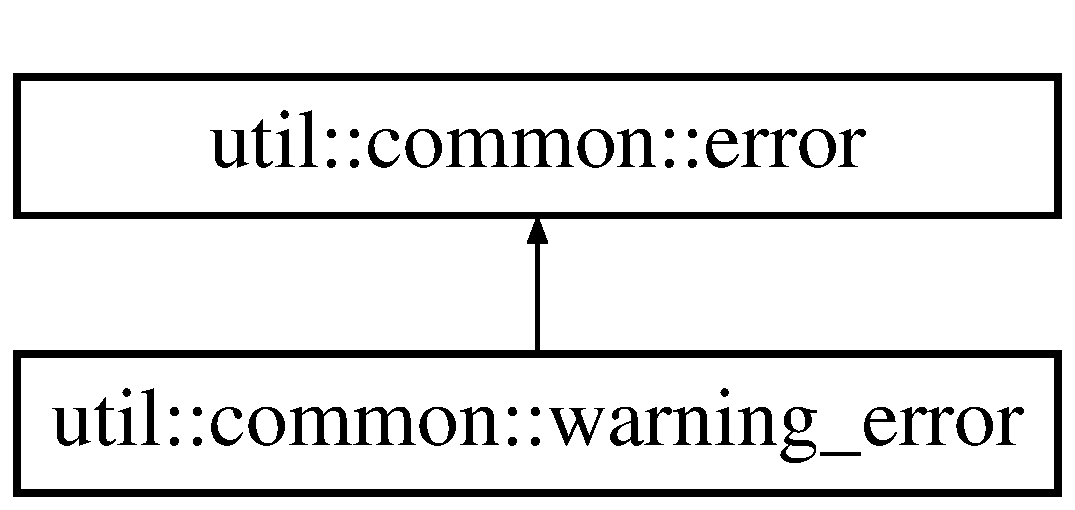
\includegraphics[height=2.000000cm]{classutil_1_1common_1_1warning__error}
\end{center}
\end{figure}
\subsection*{\-Public \-Member \-Functions}
\begin{DoxyCompactItemize}
\item 
\hypertarget{classutil_1_1common_1_1warning__error_a0904144c679c45fceabcfb6fbf550abc}{\hyperlink{classutil_1_1common_1_1warning__error_a0904144c679c45fceabcfb6fbf550abc}{warning\-\_\-error} (char const $\ast$\-\_\-error\-\_\-msg)}\label{classutil_1_1common_1_1warning__error_a0904144c679c45fceabcfb6fbf550abc}

\begin{DoxyCompactList}\small\item\em \-Constructor. \end{DoxyCompactList}\item 
\hypertarget{classutil_1_1common_1_1warning__error_a3a3f2efbe53f0daf00f5b817fd5192a0}{void \hyperlink{classutil_1_1common_1_1warning__error_a3a3f2efbe53f0daf00f5b817fd5192a0}{process} () const }\label{classutil_1_1common_1_1warning__error_a3a3f2efbe53f0daf00f5b817fd5192a0}

\begin{DoxyCompactList}\small\item\em \-Error processing method. \end{DoxyCompactList}\end{DoxyCompactItemize}


\subsection{\-Detailed \-Description}
\-The warning error class. 

\-If such an error will cause a warning to be issued to the user 

\-The documentation for this class was generated from the following file\-:\begin{DoxyCompactItemize}
\item 
/home/priyanka/\-Dataset25/src/\-G\-U\-I/\hyperlink{error_8hpp}{error.\-hpp}\end{DoxyCompactItemize}

\hypertarget{classWeightImage}{\section{\-Weight\-Image \-Class \-Reference}
\label{classWeightImage}\index{\-Weight\-Image@{\-Weight\-Image}}
}
\subsection*{\-Public \-Member \-Functions}
\begin{DoxyCompactItemize}
\item 
\hypertarget{classWeightImage_aca25af973fdd071713b9ed73971a8ef9}{{\bfseries \-Weight\-Image} (int, \-Mat)}\label{classWeightImage_aca25af973fdd071713b9ed73971a8ef9}

\item 
\hypertarget{classWeightImage_ab1cb5407d869017ff76ee38ab52fc631}{void {\bfseries fill\-Img} (int, \-Mat)}\label{classWeightImage_ab1cb5407d869017ff76ee38ab52fc631}

\item 
\hypertarget{classWeightImage_aecd8990a967993eeee9403a0e0987cf5}{void {\bfseries calculate} ()}\label{classWeightImage_aecd8990a967993eeee9403a0e0987cf5}

\end{DoxyCompactItemize}
\subsection*{\-Public \-Attributes}
\begin{DoxyCompactItemize}
\item 
\hypertarget{classWeightImage_aaca9acca67aadca4d8fa84d1c8d98490}{vector$<$ \-Mat $>$ {\bfseries matching\-Img}}\label{classWeightImage_aaca9acca67aadca4d8fa84d1c8d98490}

\item 
\hypertarget{classWeightImage_a4eaa7ea2349186695b204b8d2bc00915}{\-Mat {\bfseries \-\_\-test\-Img}}\label{classWeightImage_a4eaa7ea2349186695b204b8d2bc00915}

\item 
\hypertarget{classWeightImage_abf088bef022ae9533b835145c98512ea}{\hyperlink{classOrientedImage}{\-Oriented\-Image} {\bfseries test\-Img}}\label{classWeightImage_abf088bef022ae9533b835145c98512ea}

\item 
\hypertarget{classWeightImage_ad5eb5fe21dee1079c1b90e7d595e7860}{vector$<$ \-Mat $>$ {\bfseries \-W}}\label{classWeightImage_ad5eb5fe21dee1079c1b90e7d595e7860}

\item 
\hypertarget{classWeightImage_a84ec6c3e7d354edec8681cd1e35f8659}{vector$<$ \-Mat $>$ {\bfseries \-V}}\label{classWeightImage_a84ec6c3e7d354edec8681cd1e35f8659}

\item 
\hypertarget{classWeightImage_ac7a597c38f8209278d2e2423b3311dc8}{vector$<$ double $>$ {\bfseries v}}\label{classWeightImage_ac7a597c38f8209278d2e2423b3311dc8}

\item 
\hypertarget{classWeightImage_ad94bce97d6d2924aa8455fb3cf486292}{double {\bfseries alpha}}\label{classWeightImage_ad94bce97d6d2924aa8455fb3cf486292}

\end{DoxyCompactItemize}


\-The documentation for this class was generated from the following files\-:\begin{DoxyCompactItemize}
\item 
/home/priyanka/\-Dataset25/src/\-G\-U\-I/\-Weight\-Image.\-h\item 
/home/priyanka/\-Dataset25/src/\-G\-U\-I/\-Weight\-Image.\-cpp\end{DoxyCompactItemize}

\chapter{\-File \-Documentation}
\hypertarget{Correlation_8h}{\section{/home/priyanka/\-Dataset25/src/\-G\-U\-I/\-Correlation.h \-File \-Reference}
\label{Correlation_8h}\index{/home/priyanka/\-Dataset25/src/\-G\-U\-I/\-Correlation.\-h@{/home/priyanka/\-Dataset25/src/\-G\-U\-I/\-Correlation.\-h}}
}


\-This file calculate the positive and negative correlation between test image and matching image.  


{\ttfamily \#include \char`\"{}\-Oriented\-Image.\-h\char`\"{}}\*
\subsection*{\-Classes}
\begin{DoxyCompactItemize}
\item 
class \hyperlink{classCorrelation}{\-Correlation}
\end{DoxyCompactItemize}


\subsection{\-Detailed \-Description}
\-This file calculate the positive and negative correlation between test image and matching image. 
\hypertarget{CurvePoints_8h}{\section{/home/priyanka/\-Dataset25/src/\-G\-U\-I/\-Curve\-Points.h \-File \-Reference}
\label{CurvePoints_8h}\index{/home/priyanka/\-Dataset25/src/\-G\-U\-I/\-Curve\-Points.\-h@{/home/priyanka/\-Dataset25/src/\-G\-U\-I/\-Curve\-Points.\-h}}
}


\-This file contains the data structure used to store curve\-Points.  


{\ttfamily \#include \char`\"{}\-Drawn\-Skeleton.\-h\char`\"{}}\*
{\ttfamily \#include \char`\"{}\-Point.\-h\char`\"{}}\*
{\ttfamily \#include $<$iostream$>$}\*
{\ttfamily \#include $<$limits.\-h$>$}\*
{\ttfamily \#include $<$math.\-h$>$}\*
{\ttfamily \#include $<$set$>$}\*
{\ttfamily \#include $<$sstream$>$}\*
{\ttfamily \#include $<$fstream$>$}\*
\subsection*{\-Classes}
\begin{DoxyCompactItemize}
\item 
class \hyperlink{classCurvePoints}{\-Curve\-Points}
\end{DoxyCompactItemize}


\subsection{\-Detailed \-Description}
\-This file contains the data structure used to store curve\-Points. 
\hypertarget{Descriptor_8h}{\section{/home/priyanka/\-Dataset25/src/db/\-Descriptor.h \-File \-Reference}
\label{Descriptor_8h}\index{/home/priyanka/\-Dataset25/src/db/\-Descriptor.\-h@{/home/priyanka/\-Dataset25/src/db/\-Descriptor.\-h}}
}


\-This file contains values of descriptor and functions used to calculate and modify them.  


{\ttfamily \#include \char`\"{}opencv2/imgproc/imgproc.\-hpp\char`\"{}}\*
{\ttfamily \#include \char`\"{}opencv2/highgui/highgui.\-hpp\char`\"{}}\*
{\ttfamily \#include $<$opencv2/core/core.\-hpp$>$}\*
{\ttfamily \#include $<$iostream$>$}\*
{\ttfamily \#include $<$math.\-h$>$}\*
{\ttfamily \#include $<$vector$>$}\*
{\ttfamily \#include \char`\"{}\-Histogram.\-h\char`\"{}}\*
\subsection*{\-Classes}
\begin{DoxyCompactItemize}
\item 
class \hyperlink{classDescriptor}{\-Descriptor}
\end{DoxyCompactItemize}
\subsection*{\-Defines}
\begin{DoxyCompactItemize}
\item 
\hypertarget{Descriptor_8h_a0f8daa6d77130fa2843564393fed2981}{\#define {\bfseries \-F\-U\-N}(\-M, i, j, type)~\-M.\-at$<$type$>$(i,j)}\label{Descriptor_8h_a0f8daa6d77130fa2843564393fed2981}

\end{DoxyCompactItemize}


\subsection{\-Detailed \-Description}
\-This file contains values of descriptor and functions used to calculate and modify them. 
\hypertarget{DrawnSkeleton_8h}{\section{/home/priyanka/\-Dataset25/src/\-G\-U\-I/\-Drawn\-Skeleton.h \-File \-Reference}
\label{DrawnSkeleton_8h}\index{/home/priyanka/\-Dataset25/src/\-G\-U\-I/\-Drawn\-Skeleton.\-h@{/home/priyanka/\-Dataset25/src/\-G\-U\-I/\-Drawn\-Skeleton.\-h}}
}


\-This file contains data structure used to store user drawn skeleton joints ...  


{\ttfamily \#include $<$vector$>$}\*
{\ttfamily \#include \char`\"{}matvec.\-hpp\char`\"{}}\*
{\ttfamily \#include \char`\"{}\-Point.\-h\char`\"{}}\*
\subsection*{\-Classes}
\begin{DoxyCompactItemize}
\item 
class \hyperlink{classDrawnSkeleton}{\-Drawn\-Skeleton}
\end{DoxyCompactItemize}


\subsection{\-Detailed \-Description}
\-This file contains data structure used to store user drawn skeleton joints ... 
\hypertarget{Entry_8h}{\section{/home/priyanka/\-Dataset25/src/db/\-Entry.h \-File \-Reference}
\label{Entry_8h}\index{/home/priyanka/\-Dataset25/src/db/\-Entry.\-h@{/home/priyanka/\-Dataset25/src/db/\-Entry.\-h}}
}


\-This file describe data structure for descriptor entries stored in database.  


\subsection*{\-Classes}
\begin{DoxyCompactItemize}
\item 
class \hyperlink{classEntry}{\-Entry}
\end{DoxyCompactItemize}


\subsection{\-Detailed \-Description}
\-This file describe data structure for descriptor entries stored in database. 
\hypertarget{error_8hpp}{\section{/home/priyanka/\-Dataset25/src/\-G\-U\-I/error.hpp \-File \-Reference}
\label{error_8hpp}\index{/home/priyanka/\-Dataset25/src/\-G\-U\-I/error.\-hpp@{/home/priyanka/\-Dataset25/src/\-G\-U\-I/error.\-hpp}}
}


\-This file contains the error class definitions.  


{\ttfamily \#include $<$iostream$>$}\*
{\ttfamily \#include $<$fstream$>$}\*
{\ttfamily \#include $<$string$>$}\*
{\ttfamily \#include $<$cstdlib$>$}\*
\subsection*{\-Classes}
\begin{DoxyCompactItemize}
\item 
class \hyperlink{classutil_1_1common_1_1error}{util\-::common\-::error}
\begin{DoxyCompactList}\small\item\em \-The general error class. \end{DoxyCompactList}\item 
class \hyperlink{classutil_1_1common_1_1fatal__error}{util\-::common\-::fatal\-\_\-error}
\begin{DoxyCompactList}\small\item\em \-The fatal error class. \end{DoxyCompactList}\item 
class \hyperlink{classutil_1_1common_1_1warning__error}{util\-::common\-::warning\-\_\-error}
\begin{DoxyCompactList}\small\item\em \-The warning error class. \end{DoxyCompactList}\end{DoxyCompactItemize}
\subsection*{\-Namespaces}
\begin{DoxyCompactItemize}
\item 
namespace \hyperlink{namespaceutil}{util}
\begin{DoxyCompactList}\small\item\em \-The namespace shared by all support classes that form lib\-Util. \end{DoxyCompactList}\item 
namespace \hyperlink{namespaceutil_1_1common}{util\-::common}
\begin{DoxyCompactList}\small\item\em \-The namespace shared by error classes in lib\-Util. \end{DoxyCompactList}\end{DoxyCompactItemize}


\subsection{\-Detailed \-Description}
\-This file contains the error class definitions. 
\hypertarget{FailSafe_8h}{\section{/home/priyanka/\-Dataset25/src/\-G\-U\-I/\-Fail\-Safe.h \-File \-Reference}
\label{FailSafe_8h}\index{/home/priyanka/\-Dataset25/src/\-G\-U\-I/\-Fail\-Safe.\-h@{/home/priyanka/\-Dataset25/src/\-G\-U\-I/\-Fail\-Safe.\-h}}
}


\-This file will write all the data values that are constant after the first frame is done. \-They are needed if we close the interface and then reopen the animation frames later.  


{\ttfamily \#include \char`\"{}scribblearea.\-h\char`\"{}}\*
\subsection*{\-Classes}
\begin{DoxyCompactItemize}
\item 
class \hyperlink{classFailSafe}{\-Fail\-Safe}
\end{DoxyCompactItemize}


\subsection{\-Detailed \-Description}
\-This file will write all the data values that are constant after the first frame is done. \-They are needed if we close the interface and then reopen the animation frames later. 
\hypertarget{Grid_8h}{\section{/home/priyanka/\-Dataset25/src/\-G\-U\-I/\-Grid.h \-File \-Reference}
\label{Grid_8h}\index{/home/priyanka/\-Dataset25/src/\-G\-U\-I/\-Grid.\-h@{/home/priyanka/\-Dataset25/src/\-G\-U\-I/\-Grid.\-h}}
}


\-This file will store the patch location of different patches of image.  


{\ttfamily \#include \char`\"{}\-Cell.\-cpp\char`\"{}}\*
\subsection*{\-Classes}
\begin{DoxyCompactItemize}
\item 
class \hyperlink{classGrid}{\-Grid}
\end{DoxyCompactItemize}


\subsection{\-Detailed \-Description}
\-This file will store the patch location of different patches of image. 
\hypertarget{Hash_8h}{\section{/home/priyanka/\-Dataset25/src/\-G\-U\-I/\-Hash.h \-File \-Reference}
\label{Hash_8h}\index{/home/priyanka/\-Dataset25/src/\-G\-U\-I/\-Hash.\-h@{/home/priyanka/\-Dataset25/src/\-G\-U\-I/\-Hash.\-h}}
}


\-This file describe data structure for hash function.  


{\ttfamily \#include $<$iostream$>$}\*
{\ttfamily \#include $<$stdlib.\-h$>$}\*
{\ttfamily \#include $<$math.\-h$>$}\*
{\ttfamily \#include $<$vector$>$}\*
\subsection*{\-Classes}
\begin{DoxyCompactItemize}
\item 
class \hyperlink{classHash}{\-Hash}
\end{DoxyCompactItemize}


\subsection{\-Detailed \-Description}
\-This file describe data structure for hash function. 
\hypertarget{Histogram_8h}{\section{/home/priyanka/\-Dataset25/src/db/\-Histogram.h \-File \-Reference}
\label{Histogram_8h}\index{/home/priyanka/\-Dataset25/src/db/\-Histogram.\-h@{/home/priyanka/\-Dataset25/src/db/\-Histogram.\-h}}
}


\-This file store values of 3\-D histogram and functions to calculate and modify them.  


{\ttfamily \#include \char`\"{}opencv2/imgproc/imgproc.\-hpp\char`\"{}}\*
{\ttfamily \#include \char`\"{}opencv2/highgui/highgui.\-hpp\char`\"{}}\*
{\ttfamily \#include $<$opencv2/core/core.\-hpp$>$}\*
{\ttfamily \#include $<$iostream$>$}\*
{\ttfamily \#include $<$math.\-h$>$}\*
{\ttfamily \#include $<$vector$>$}\*
\subsection*{\-Classes}
\begin{DoxyCompactItemize}
\item 
class \hyperlink{classHistogram}{\-Histogram}
\end{DoxyCompactItemize}


\subsection{\-Detailed \-Description}
\-This file store values of 3\-D histogram and functions to calculate and modify them. 
\hypertarget{ImageVotes_8h}{\section{/home/priyanka/\-Dataset25/src/\-G\-U\-I/\-Image\-Votes.h \-File \-Reference}
\label{ImageVotes_8h}\index{/home/priyanka/\-Dataset25/src/\-G\-U\-I/\-Image\-Votes.\-h@{/home/priyanka/\-Dataset25/src/\-G\-U\-I/\-Image\-Votes.\-h}}
}


\-This file find the maximum votes per image.  


{\ttfamily \#include \char`\"{}\-Grid.\-h\char`\"{}}\*
{\ttfamily \#include $<$vector$>$}\*
\subsection*{\-Classes}
\begin{DoxyCompactItemize}
\item 
class \hyperlink{classImageVotes}{\-Image\-Votes}
\end{DoxyCompactItemize}


\subsection{\-Detailed \-Description}
\-This file find the maximum votes per image. 
\hypertarget{Index_8h}{\section{/home/priyanka/\-Dataset25/src/\-G\-U\-I/\-Index.h \-File \-Reference}
\label{Index_8h}\index{/home/priyanka/\-Dataset25/src/\-G\-U\-I/\-Index.\-h@{/home/priyanka/\-Dataset25/src/\-G\-U\-I/\-Index.\-h}}
}


\-This file describe data structure for descriptor entries stored in database.  


{\ttfamily \#include $<$iostream$>$}\*
{\ttfamily \#include $<$math.\-h$>$}\*
{\ttfamily \#include $<$vector$>$}\*
{\ttfamily \#include \char`\"{}\-Table.\-h\char`\"{}}\*
\subsection*{\-Classes}
\begin{DoxyCompactItemize}
\item 
class \hyperlink{classIndex}{\-Index}
\end{DoxyCompactItemize}


\subsection{\-Detailed \-Description}
\-This file describe data structure for descriptor entries stored in database. 
\hypertarget{MatchingImage_8h}{\section{/home/priyanka/\-Dataset25/src/\-G\-U\-I/\-Matching\-Image.h \-File \-Reference}
\label{MatchingImage_8h}\index{/home/priyanka/\-Dataset25/src/\-G\-U\-I/\-Matching\-Image.\-h@{/home/priyanka/\-Dataset25/src/\-G\-U\-I/\-Matching\-Image.\-h}}
}


\-This file find the most matching images from database corresponding to user drawing and blend them together to generate shadow image.  


{\ttfamily \#include \char`\"{}\-Descriptor.\-h\char`\"{}}\*
{\ttfamily \#include \char`\"{}\-Index\-Storage.\-h\char`\"{}}\*
{\ttfamily \#include \char`\"{}\-Image\-Votes.\-h\char`\"{}}\*
{\ttfamily \#include \char`\"{}\-Weight\-Image.\-h\char`\"{}}\*
{\ttfamily \#include \char`\"{}shift.\-h\char`\"{}}\*
\subsection*{\-Classes}
\begin{DoxyCompactItemize}
\item 
class \hyperlink{classMatchingImage}{\-Matching\-Image}
\end{DoxyCompactItemize}


\subsection{\-Detailed \-Description}
\-This file find the most matching images from database corresponding to user drawing and blend them together to generate shadow image. 
\hypertarget{matvec_8hpp}{\section{/home/priyanka/\-Dataset25/src/\-G\-U\-I/matvec.hpp \-File \-Reference}
\label{matvec_8hpp}\index{/home/priyanka/\-Dataset25/src/\-G\-U\-I/matvec.\-hpp@{/home/priyanka/\-Dataset25/src/\-G\-U\-I/matvec.\-hpp}}
}


\-This file contains 3 vector and 2 matrix class definitions \-The vector classes are vec2, vec3 \& vec4. \-The matrix classes are mat33 \& mat44.  


{\ttfamily \#include $<$cstdio$>$}\*
{\ttfamily \#include $<$string$>$}\*
\subsection*{\-Classes}
\begin{DoxyCompactItemize}
\item 
class \hyperlink{classutil_1_1math_1_1vec2}{util\-::math\-::vec2}
\begin{DoxyCompactList}\small\item\em \-This is a general 2\-D vector class. \end{DoxyCompactList}\item 
class \hyperlink{classutil_1_1math_1_1vec3}{util\-::math\-::vec3}
\begin{DoxyCompactList}\small\item\em \-This is a general 3\-D vector class. \end{DoxyCompactList}\item 
class \hyperlink{classutil_1_1math_1_1vec4}{util\-::math\-::vec4}
\begin{DoxyCompactList}\small\item\em \-This is a general 4\-D vector class. \end{DoxyCompactList}\item 
class \hyperlink{classutil_1_1math_1_1mat33}{util\-::math\-::mat33}
\begin{DoxyCompactList}\small\item\em \-This is a general 3x3 matrix class. \end{DoxyCompactList}\item 
class \hyperlink{classutil_1_1math_1_1mat44}{util\-::math\-::mat44}
\begin{DoxyCompactList}\small\item\em \-This is a general 4x4 matrix class. \end{DoxyCompactList}\end{DoxyCompactItemize}
\subsection*{\-Namespaces}
\begin{DoxyCompactItemize}
\item 
namespace \hyperlink{namespaceutil}{util}
\begin{DoxyCompactList}\small\item\em \-The namespace shared by all support classes that form lib\-Util. \end{DoxyCompactList}\item 
namespace \hyperlink{namespaceutil_1_1math}{util\-::math}
\begin{DoxyCompactList}\small\item\em \-The namespace containing all the math classes in lib\-Util. \end{DoxyCompactList}\end{DoxyCompactItemize}
\subsection*{\-Enumerations}
\begin{DoxyCompactItemize}
\item 
enum \{ {\bfseries \-X}, 
{\bfseries \-Y}, 
{\bfseries \-Z}, 
{\bfseries \-W}
 \}
\begin{DoxyCompactList}\small\item\em \-The \-X,\-Y,\-Z,\-W coordinates. \end{DoxyCompactList}\end{DoxyCompactItemize}
\subsection*{\-Variables}
\begin{DoxyCompactItemize}
\item 
\hypertarget{namespaceutil_1_1math_a341939326d8a0061b87c80ad65ee2bbb}{const double \hyperlink{namespaceutil_1_1math_a341939326d8a0061b87c80ad65ee2bbb}{util\-::math\-::\-E\-P\-S\-I\-L\-O\-N} = 1e-\/6}\label{namespaceutil_1_1math_a341939326d8a0061b87c80ad65ee2bbb}

\begin{DoxyCompactList}\small\item\em \-This is used for comparison amongst floating pt. values. \end{DoxyCompactList}\end{DoxyCompactItemize}


\subsection{\-Detailed \-Description}
\-This file contains 3 vector and 2 matrix class definitions \-The vector classes are vec2, vec3 \& vec4. \-The matrix classes are mat33 \& mat44. \-All standard arithmetic operations are defined. '$\ast$' is used for the dot product of two vectors and two matrices. '$^\wedge$' is used for the cross product of two vectors.

\-Additional functions include length(), normalize(), homogenize for vectors, and print(), set(), map() for all classes.

\-There are the transpose() \& inverse for matrices, but note that they do not actually change the matrix.

\-When multiplied with a matrix, a vector is treated as a row vector if it precedes the matrix (v$\ast$\-M), and as a column vector if it follows the matrix (\-M$\ast$v).

\-Matrices are stored in row-\/major form.

\-A vector of one dimension (2d, 3d, or 4d) can be cast to a vector of a higher or lower dimension. \-If casting to a higher dimension, the new component is set by default to 1.\-0, unless a value is specified\-: vec3 a(1.\-0, 2.\-0, 3.\-0 ); vec4 b( a, 4.\-0 ); // now b == \{1.\-0, 2.\-0, 3.\-0, 4.\-0\}; \-When casting to a lower dimension, the vector is homogenized in the lower dimension. \-E.\-g., if a 4d \{\-X,\-Y,\-Z,\-W\} is cast to 3d, the resulting vector is \{\-X/\-W, \-Y/\-W, \-Z/\-W\}. \-It is up to the user to ensure the fourth component is not zero before casting.

\-Authors\-: \-Jean-\/\-Francois \-Doue (\-Graphics \-Gems \-I\-V), \-Paul \-Rademacher \-Revised\-: \-Parag \-Chaudhuri 
\hypertarget{OrientedImage_8h}{\section{/home/priyanka/\-Dataset25/src/\-G\-U\-I/\-Oriented\-Image.h \-File \-Reference}
\label{OrientedImage_8h}\index{/home/priyanka/\-Dataset25/src/\-G\-U\-I/\-Oriented\-Image.\-h@{/home/priyanka/\-Dataset25/src/\-G\-U\-I/\-Oriented\-Image.\-h}}
}


\-This file contains the data structure used to store curve\-Points.  


{\ttfamily \#include \char`\"{}opencv2/imgproc/imgproc.\-hpp\char`\"{}}\*
{\ttfamily \#include \char`\"{}opencv2/highgui/highgui.\-hpp\char`\"{}}\*
{\ttfamily \#include $<$opencv2/core/core.\-hpp$>$}\*
{\ttfamily \#include $<$iostream$>$}\*
{\ttfamily \#include $<$math.\-h$>$}\*
{\ttfamily \#include \char`\"{}\-Steerable.\-h\char`\"{}}\*
\subsection*{\-Classes}
\begin{DoxyCompactItemize}
\item 
class \hyperlink{classOrientedImage}{\-Oriented\-Image}
\end{DoxyCompactItemize}


\subsection{\-Detailed \-Description}
\-This file contains the data structure used to store curve\-Points. 
\hypertarget{ResultSet_8h}{\section{/home/priyanka/\-Dataset25/src/db/\-Result\-Set.h \-File \-Reference}
\label{ResultSet_8h}\index{/home/priyanka/\-Dataset25/src/db/\-Result\-Set.\-h@{/home/priyanka/\-Dataset25/src/db/\-Result\-Set.\-h}}
}


\-This file consist of matching result patches found for user drawn image.  


{\ttfamily \#include $<$iostream$>$}\*
{\ttfamily \#include \char`\"{}\-Entry.\-h\char`\"{}}\*
{\ttfamily \#include $<$unordered\-\_\-map$>$}\*
{\ttfamily \#include $<$iterator$>$}\*
{\ttfamily \#include $<$vector$>$}\*
\subsection*{\-Classes}
\begin{DoxyCompactItemize}
\item 
class \hyperlink{classHasher}{\-Hasher}
\item 
class \hyperlink{classEqualFn}{\-Equal\-Fn}
\item 
class \hyperlink{classResultSet}{\-Result\-Set}
\end{DoxyCompactItemize}


\subsection{\-Detailed \-Description}
\-This file consist of matching result patches found for user drawn image. 
\hypertarget{RetrievedSkeleton_8h}{\section{/home/priyanka/\-Dataset25/src/\-G\-U\-I/\-Retrieved\-Skeleton.h \-File \-Reference}
\label{RetrievedSkeleton_8h}\index{/home/priyanka/\-Dataset25/src/\-G\-U\-I/\-Retrieved\-Skeleton.\-h@{/home/priyanka/\-Dataset25/src/\-G\-U\-I/\-Retrieved\-Skeleton.\-h}}
}


\-This file will store the datavalues read from converted bvh file.  


{\ttfamily \#include \char`\"{}\-Drawn\-Skeleton.\-h\char`\"{}}\*
{\ttfamily \#include $<$vector$>$}\*
{\ttfamily \#include $<$limits.\-h$>$}\*
{\ttfamily \#include $<$fstream$>$}\*
{\ttfamily \#include $<$iostream$>$}\*
{\ttfamily \#include $<$sstream$>$}\*
{\ttfamily \#include $<$math.\-h$>$}\*
\subsection*{\-Classes}
\begin{DoxyCompactItemize}
\item 
class \hyperlink{classRetrievedSkeleton}{\-Retrieved\-Skeleton}
\end{DoxyCompactItemize}


\subsection{\-Detailed \-Description}
\-This file will store the datavalues read from converted bvh file. 
\hypertarget{scribblearea_8h}{\section{/home/priyanka/\-Dataset25/src/\-G\-U\-I/scribblearea.h \-File \-Reference}
\label{scribblearea_8h}\index{/home/priyanka/\-Dataset25/src/\-G\-U\-I/scribblearea.\-h@{/home/priyanka/\-Dataset25/src/\-G\-U\-I/scribblearea.\-h}}
}


\-This file basically deals with all the interface related functions.  


{\ttfamily \#include $<$\-Q\-Color$>$}\*
{\ttfamily \#include $<$\-Q\-Image$>$}\*
{\ttfamily \#include $<$\-Q\-Point$>$}\*
{\ttfamily \#include $<$\-Q\-Widget$>$}\*
{\ttfamily \#include $<$\-Q\-Key\-Event$>$}\*
{\ttfamily \#include $<$vector$>$}\*
{\ttfamily \#include $<$fstream$>$}\*
{\ttfamily \#include \char`\"{}\-Matching\-Image.\-h\char`\"{}}\*
{\ttfamily \#include \char`\"{}\-Retrieved\-Skeleton.\-h\char`\"{}}\*
{\ttfamily \#include \char`\"{}\-Curve\-Points.\-h\char`\"{}}\*
\subsection*{\-Classes}
\begin{DoxyCompactItemize}
\item 
class \hyperlink{classScribbleArea}{\-Scribble\-Area}
\end{DoxyCompactItemize}


\subsection{\-Detailed \-Description}
\-This file basically deals with all the interface related functions. 
\hypertarget{Table_8h}{\section{/home/priyanka/\-Dataset25/src/db/\-Table.h \-File \-Reference}
\label{Table_8h}\index{/home/priyanka/\-Dataset25/src/db/\-Table.\-h@{/home/priyanka/\-Dataset25/src/db/\-Table.\-h}}
}


\-This file contain all the entries generated for different patches of all the images in database.  


{\ttfamily \#include $<$iostream$>$}\*
{\ttfamily \#include $<$math.\-h$>$}\*
{\ttfamily \#include $<$vector$>$}\*
{\ttfamily \#include $<$unordered\-\_\-map$>$}\*
{\ttfamily \#include \char`\"{}\-Hash.\-h\char`\"{}}\*
{\ttfamily \#include \char`\"{}\-Result\-Set.\-h\char`\"{}}\*
\subsection*{\-Classes}
\begin{DoxyCompactItemize}
\item 
class \hyperlink{classTable}{\-Table}
\end{DoxyCompactItemize}


\subsection{\-Detailed \-Description}
\-This file contain all the entries generated for different patches of all the images in database. 
\hypertarget{WeightImage_8h}{\section{/home/priyanka/\-Dataset25/src/\-G\-U\-I/\-Weight\-Image.h \-File \-Reference}
\label{WeightImage_8h}\index{/home/priyanka/\-Dataset25/src/\-G\-U\-I/\-Weight\-Image.\-h@{/home/priyanka/\-Dataset25/src/\-G\-U\-I/\-Weight\-Image.\-h}}
}


\-This file contains the \-Weight \-Matrix.  


{\ttfamily \#include \char`\"{}\-Correlation.\-h\char`\"{}}\*
\subsection*{\-Classes}
\begin{DoxyCompactItemize}
\item 
class \hyperlink{classWeightImage}{\-Weight\-Image}
\end{DoxyCompactItemize}


\subsection{\-Detailed \-Description}
\-This file contains the \-Weight \-Matrix. 
\printindex
\end{document}
